%%===========================================================%%
%%                                                           %%
%%                   SYSTEMATIC ERRORS                       %%
%%                                                           %%
%%===========================================================%%


\chapter{Systematic uncertainties}\label{chap:systematicErrors}
In this chapter we describe the common systematic uncertainties for two analyses~\cite{AnalysisNoteRafal,AnalysisNoteLukasz}, related to: TPC track reconstruction efficiency, TOF matching efficiency and RP track reconstruction efficiency.
\section{TPC track reconstruction efficiency}\label{sec:tpcSystematics}
\subsection{Embedding (pile-up) effect}\label{subsec:TpcEffSystPileUp}
One major difference between simulation and real data is the presence of pile-up
events. The average number of pile-up tracks in
a triggering event is proportional to the BBC coincidence rate as shown in Fig.~\ref{fig:events_bbc_and_meanGlobalTracks}. It is expected that
the difference between simulation and real data drops at lower BBC rates, and the
effects of pile-up tracks could be much reduced by fitting the tracking efficiency as a
function of BBC rate and using the~extrapolated value at zero luminosity to compare
with simulation.
\newline
%---------------------------
\begin{wrapfigure}{r}{0.45\textwidth}\vspace*{-9pt}
	\centering
	\includegraphics[width=0.45\textwidth, page=5]{graphics/systematicsEfficiency/bbc_and/Out.pdf}
	\caption[Number of events in embedded MC as a function of BBC\_AND rate.]
	{Number of events in embedded MC as a function of BBC\_AND rate. The black and red lines represent the events with \mbox{$<\text{BBC\_AND}>=700$~kHz} and \mbox{$<\text{BBC\_AND}>=1400$~kHz},  respectively.}
	\label{fig:events_bbc_and}%\vspace*{-29pt}
\end{wrapfigure}
%---------------------------
\noindent The embedded MC was divided into two samples due to mean BBC\_AND rate: \mbox{$<\text{BBC\_AND}>=700$~kHz} and \mbox{$<\text{BBC\_AND}>=1400$~kHz}, as shown in Fig.~\ref{fig:events_bbc_and}. Next, the track reconstruction efficiency was calculated for those two samples and no-pile-up MC corresponding to them. The difference between TPC track reconstruction efficiences for pile-up and no-pile-up MCs was calculated as:
\begin{equation}
	\Delta\epsilon_{ TPC}^{1400/700\text{ kHz}} = \frac{N_{reco}^{no-pile-up}-N_{reco}^{pile-up}}{N_{gen}}\\
	\label{eq:tpcSyst}
\end{equation}
where:\\
$N_{gen}$-number of MC tracks,\\
$N_{reco}^{no-pile-up}$ - number of reconstructed tracks, matched with MC tracks in no-pile-up MC,\\
$N_{reco}^{pile-up}$ - number of reconstructed tracks, matched with MC tracks in pile-up MC.


The difference between high and low pile-up runs is given by:
\begin{equation}
\Delta\epsilon_{ TPC} =\Delta\epsilon_{ TPC}^{1400\text{ kHz}}-2\cdot\Delta\epsilon_{ TPC}^{700\text{ kHz}}
\label{eq:tpcSystDifference}
\end{equation}
Finally, above difference, shown in  \Cref{fig:systError1Dtpc,fig:systError2Dtpc} for $\pi^\pm$, varies between $2-3\%$ and was taken as systematic uncertainty related to TPC track reconstruction efficiency.
%\vspace{10em}
\begin{figure}[hb]
	\centering
	\parbox{0.495\textwidth}{
		\centering
		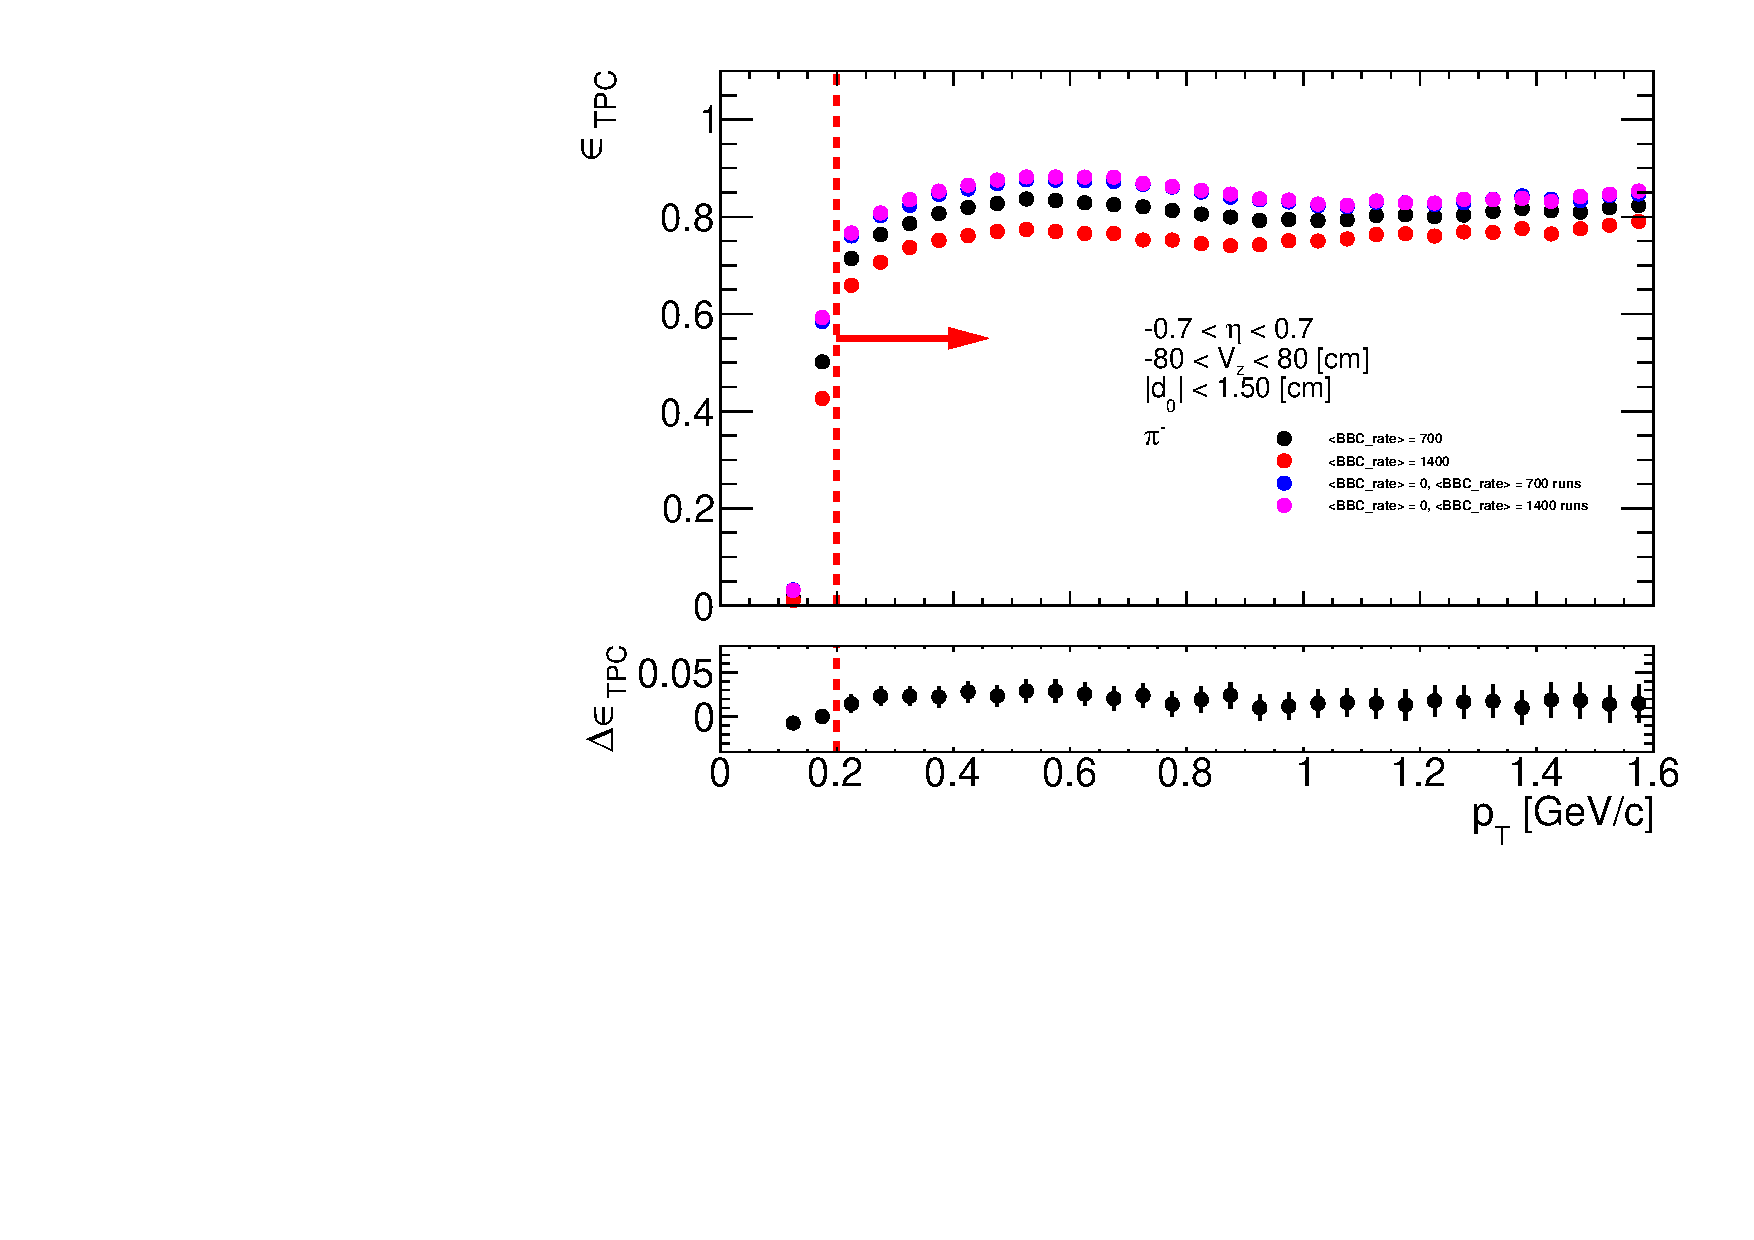
\includegraphics[width=\linewidth,page=1]{graphics/systematicsEfficiency/bbc_and/tpcEffi_d0_1_5_etapt_1.pdf}\\
	}~
	\parbox{0.495\textwidth}{
		\centering
		\includegraphics[width=\linewidth,page=2]{graphics/systematicsEfficiency/bbc_and/tpcEffi_d0_1_5_etapt_1.pdf}\\
	}%
	\caption[$\pi^\pm$ TPC track reconstruction efficiency as a function of $p_T$ $\left(|\eta|<0.7, |V_z|<80\text{ cm}\right)$ for embedded MC samples with \mbox{$<\text{BBC\_AND}>=700$~kHz} and \mbox{$<\text{BBC\_AND}>=1400$~kHz}]{$\pi^\pm$ TPC track reconstruction efficiency as a function of $p_T$ $\left(|\eta|<0.7, |V_z|<80\text{ cm}\right)$ for embedded MC samples with \mbox{$<\text{BBC\_AND}>=700$~kHz} and \mbox{$<\text{BBC\_AND}>=1400$~kHz}. The efficiences from corresponding no-pile-up MC samples were also shown. Additionally, the differences  from Eq. \ref{eq:tpcSystDifference} were drawn in the bottom of each plot.}
	\label{fig:systError1Dtpc}
\end{figure}
\begin{figure}[H]
	\centering
	\parbox{0.495\textwidth}{
		\centering
		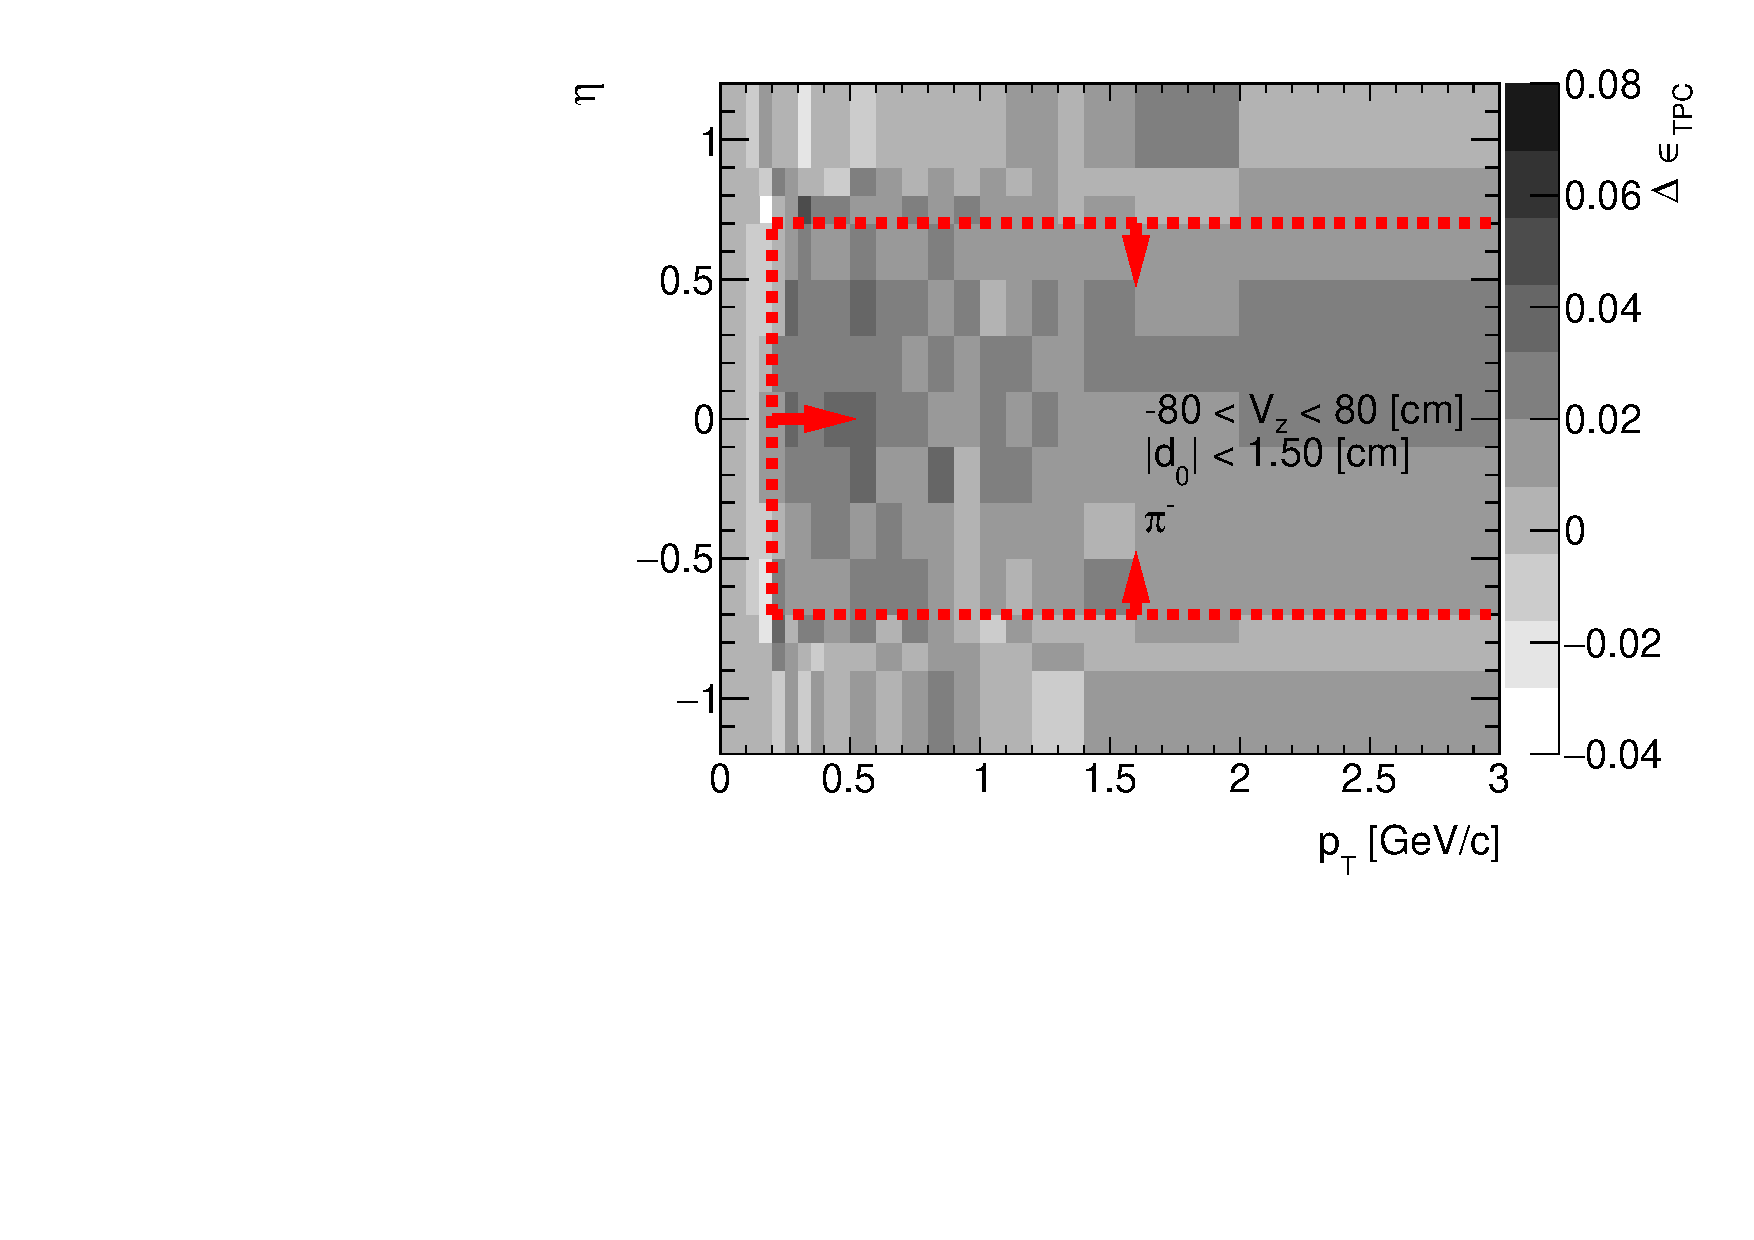
\includegraphics[width=\linewidth,page=1]{graphics/systematicsEfficiency/bbc_and/tpcEffi_d0_1_5_etapt_12D.pdf}\\
	}~
	\parbox{0.495\textwidth}{
		\centering
		\includegraphics[width=\linewidth,page=2]{graphics/systematicsEfficiency/bbc_and/tpcEffi_d0_1_5_etapt_12D.pdf}\\
	}~
	\caption[The difference $\Delta\epsilon_{ TPC} =\Delta\epsilon_{ TPC}^{1400\text{ kHz}}-2\cdot\Delta\epsilon_{ TPC}^{700\text{ kHz}}$ for $\pi^\pm$ as a function of $p_T$ and $\eta$ $\left(|V_z|<80\text{ cm}\right)$]{The difference $\Delta\epsilon_{ TPC} =\Delta\epsilon_{ TPC}^{1400\text{ kHz}}-2\cdot\Delta\epsilon_{ TPC}^{700\text{ kHz}}$ for $\pi^\pm$ as a function of $p_T$ and $\eta$ $\left(|V_z|<80\text{ cm}\right)$. }
	\label{fig:systError2Dtpc}
\end{figure}

%%%%%%%%%%
%tutaj pisac 
%%%%%%%%%%%





The comparison of the BBC\_AND rate for SD and CD in the data and embedded MC is shown in Fig.~\ref{fig:systErrorEmbDataRate}. The mean BBC\_AND rate varies between embedded MC and data by about  $15\%$ and $10\%$ for SD and CD, respectively. As shown in Fig.~\ref{fig:systError1Dtpc}, 
the effect of the embedding on the TPC track reconstruction efficiency is about $10\%$.  Thus, the additional systematic error due to different mean BBC\_AND rate in the data and embedded MC was introduced as about $1.5\%$ and $1\%$ for SD and CD, respectively.
	
\begin{figure}[H]
	\centering
	\parbox{0.495\textwidth}{
		\centering
		\includegraphics[width=\linewidth,page=9]{graphics/systematicsEfficiency/bbc_and/Out.pdf}\\
	}~
	\parbox{0.495\textwidth}{
		\centering
		\includegraphics[width=\linewidth,page=10]{graphics/systematicsEfficiency/bbc_and/Out.pdf}\\
	}\\
	\parbox{0.495\textwidth}{
		\centering
		\includegraphics[width=\linewidth,page=11]{graphics/systematicsEfficiency/bbc_and/Out.pdf}\\
	}
	\parbox{0.495\textwidth}{
		\centering
		\includegraphics[width=\linewidth,page=12]{graphics/systematicsEfficiency/bbc_and/Out.pdf}\\
	}
	\caption[Comparison of the BBC\_AND rate in the data  and   embedded MC for SD and CD.]{Comparison of the BBC\_AND rate in the data  and   embedded MC for SD and CD. The mean BBC\_AND rate for data and MC is given on each plot.}
	\label{fig:systErrorEmbDataRate}
\end{figure}

\subsection{Dead material effect on TPC track reconstruction efficiency}\label{sec:deadMaterialSystematics}
The amount of dead material in front of TPC differs up to $25\%$ between data and simulation (see Sec.~\ref{chap:deadMaterial}). First, the~amount of lost particles, $\delta\epsilon_{ TPC}$, due to the interaction with dead material in front of TPC was estimated using  no-pile-up  MC samples. The sample result for $\pi^-$ in CD and SD is shown in Fig. \ref{fig:dead_materialCDSD3D}. The remaning plots for other $z$-vertex bins and other particles are contained  in Appendix \ref{appendix:deadMaterial}.
The symmetric systematic uncertainty on the TPC track reconstruction efficiency due to dead material was introduced as $\pm 0.25 \cdot\delta\epsilon_{ TPC}$.
In Fig. \ref{fig:dead_materialCDSD1D}  the systematic uncertainty is shown for each particle species in CD and SD as a~function of $p_T$ $\left(|\eta|<0.7, |V_{z}|<80 \text{ cm}\right)$. 

\begin{figure}[h!]%\vspace{-10pt}
	\centering
	\includegraphics[width=0.9\linewidth,page=9]{graphics/systematicsEfficiency/deadMaterial/secondaries_Unbinned_SDCD_.pdf}\vspace*{-8pt}
	\caption[The amount of lost $\pi^-$ due to the interaction with dead material in front of TPC as a function of $p_T$, $\eta$ in sample $z$-vertex bin in CD and SD]{The amount of lost $\pi^-$ due to the interaction with dead material in front of TPC. Sample plot represents the fraction of lost $\pi^-$, $\delta\epsilon_{ TPC}$ ($z$-axis), as a function of true particle pseudorapidity $\eta$ ($y$-axis) and transverse momentum $p_{T}$ ($x$-axis) in single $z$-vertex bin. Red lines and arrows indicate region accepted in the analysis.}\label{fig:dead_materialCDSD3D}
\end{figure}
\begin{figure}[hb]
\centering
\parbox{0.49\textwidth}{
  \centering
  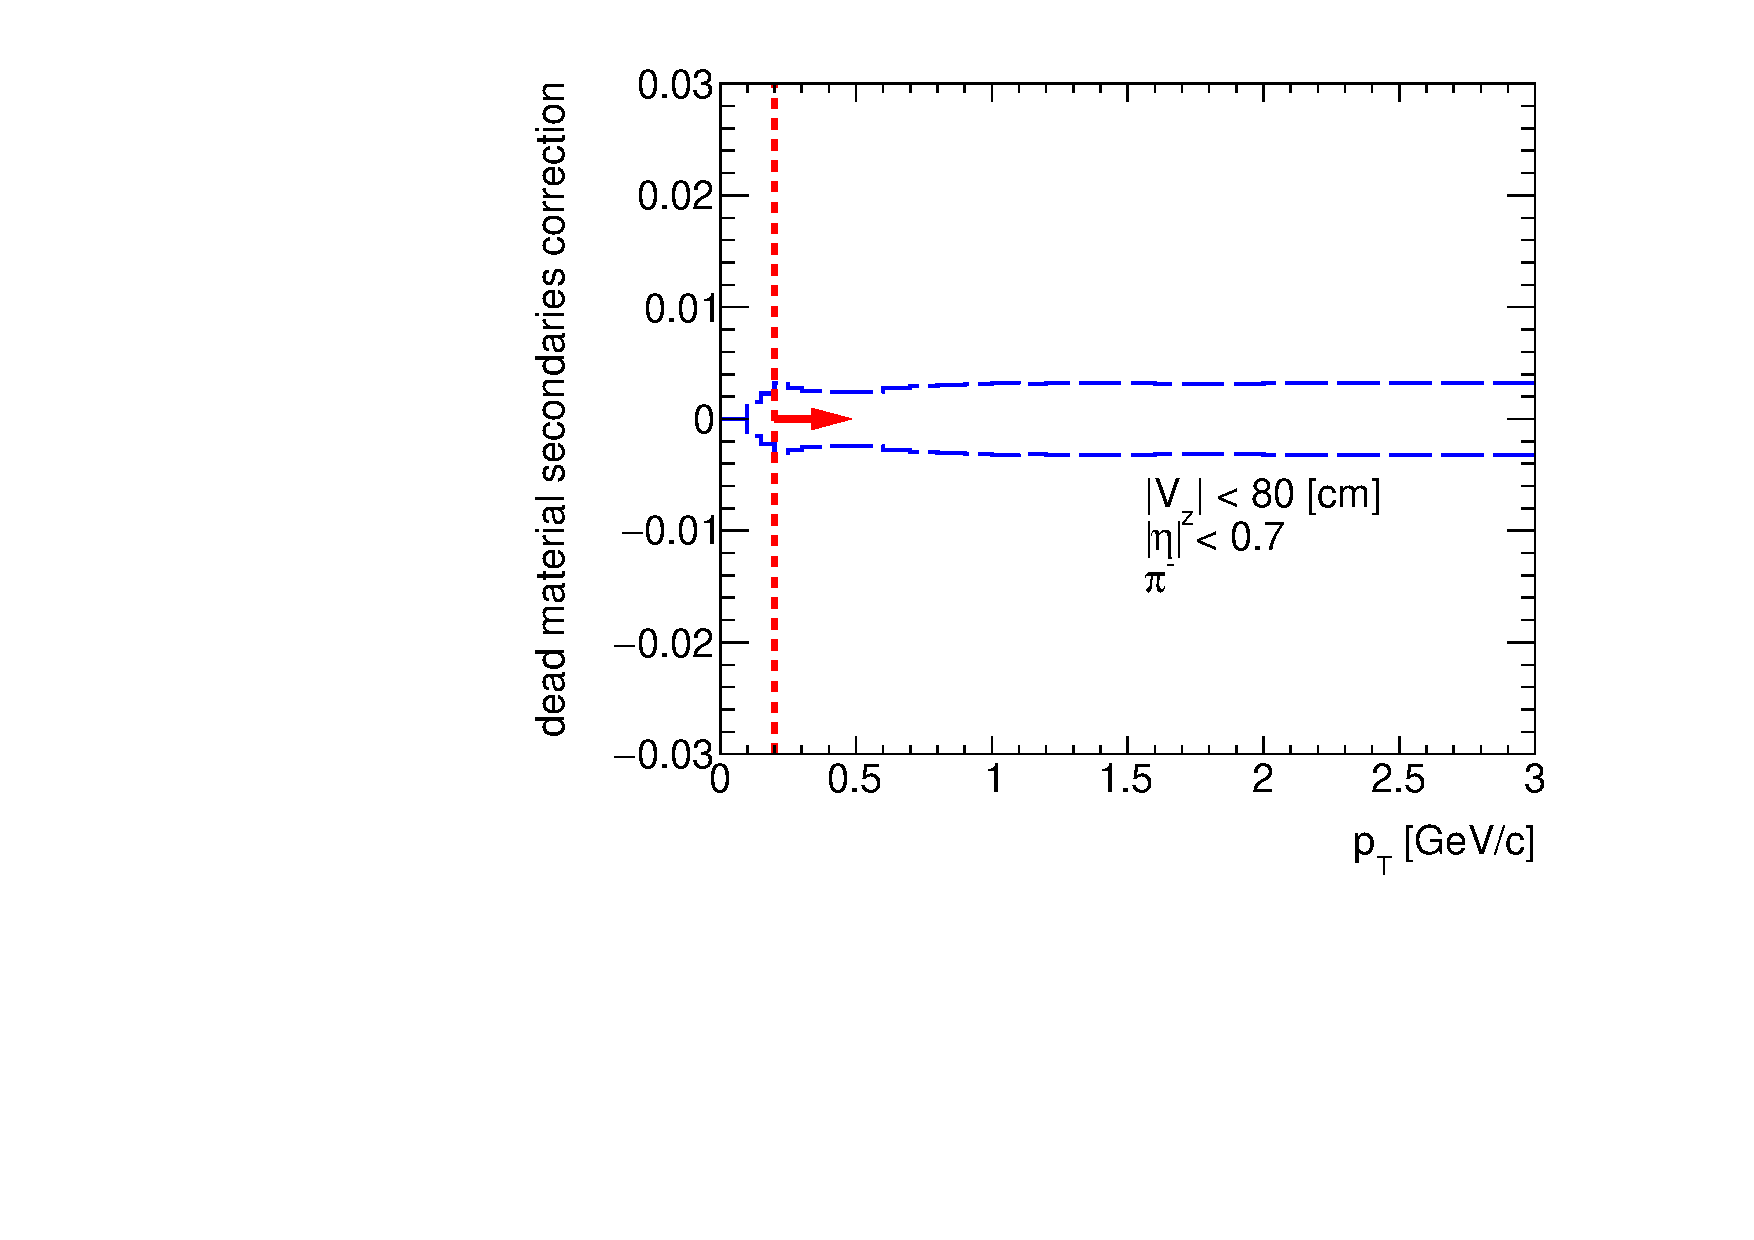
\includegraphics[width=\linewidth,page=1]{graphics/systematicsEfficiency/deadMaterial/secondaries_Unbinned_SDCD_1D.pdf}\\
  \includegraphics[width=\linewidth,page=2]{graphics/systematicsEfficiency/deadMaterial/secondaries_Unbinned_SDCD_1D.pdf}\\
  \includegraphics[width=\linewidth,page=3]{graphics/systematicsEfficiency/deadMaterial/secondaries_Unbinned_SDCD_1D.pdf}\\
  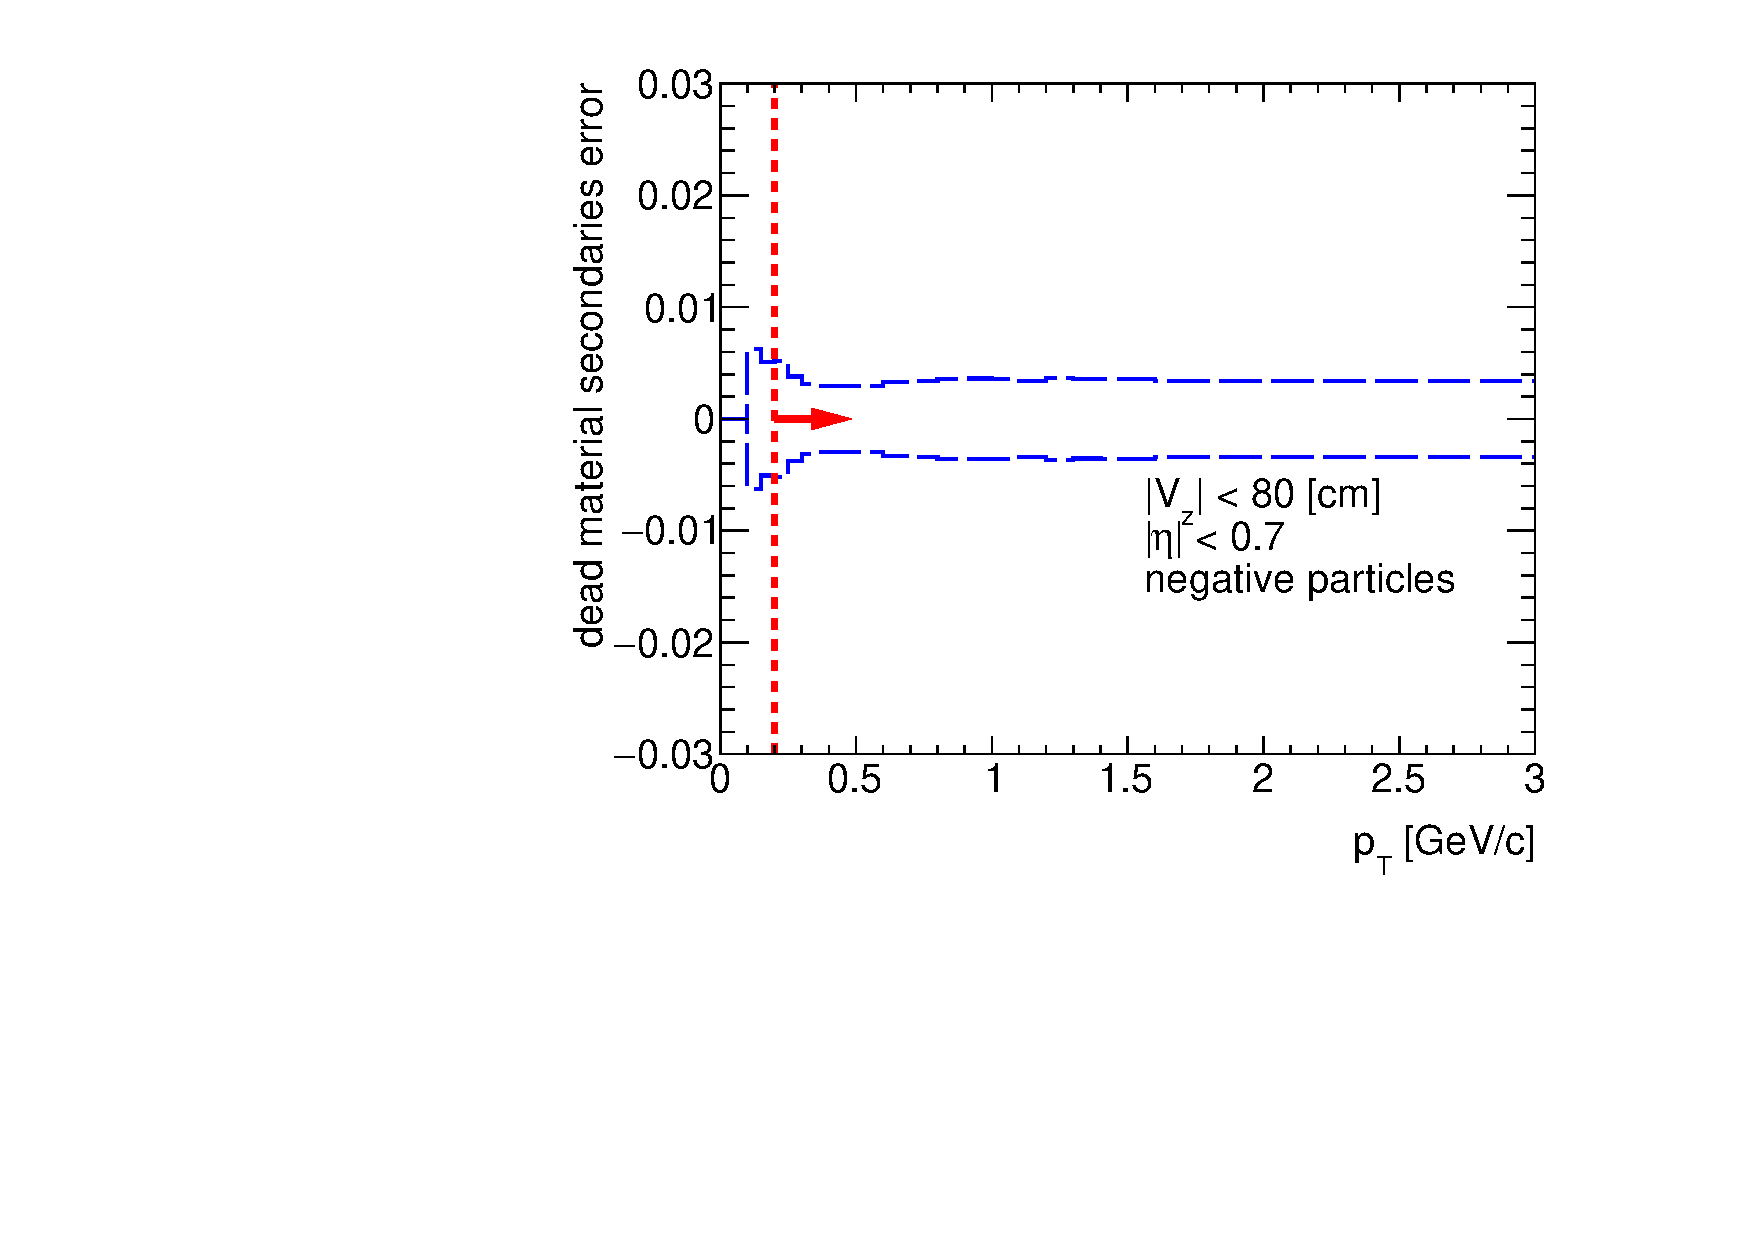
\includegraphics[width=\linewidth,page=1]{graphics/systematicsEfficiency/deadMaterial/secondaries_Unbinned_Charged_SDCD1D.pdf}\\
}~
\parbox{0.49\textwidth}{
  \centering
  \includegraphics[width=\linewidth,page=4]{graphics/systematicsEfficiency/deadMaterial/secondaries_Unbinned_SDCD_1D.pdf}\\
  \includegraphics[width=\linewidth,page=5]{graphics/systematicsEfficiency/deadMaterial/secondaries_Unbinned_SDCD_1D.pdf}\\
  \includegraphics[width=\linewidth,page=6]{graphics/systematicsEfficiency/deadMaterial/secondaries_Unbinned_SDCD_1D.pdf}\\
  \includegraphics[width=\linewidth,page=2]{graphics/systematicsEfficiency/deadMaterial/secondaries_Unbinned_Charged_SDCD1D.pdf}
}%
\caption[The systematic uncertainty to the TPC track reconstruction efficiency due to  amount of dead material in front of TPC using MC samples for CD and SD]{The systematic uncertainty to the TPC track reconstruction efficiency due to  amount of dead material in front of TPC using MC samples for CD and SD. Each plot represents the systematic uncertainty as a~function of true particle $p_T$ $\left(|\eta|<0.7, |V_{z}|<80 \text{ cm}\right)$ for given particle species: $\pi^-$,$\pi^+$, $K^-$, $K^+$, $\bar{p}$, $p$, negative and positive particles without identification. Red lines and arrows indicate region accepted in the analysis.}\label{fig:dead_materialCDSD1D}
\end{figure}



\section{TOF matching efficiency}\label{sec:tofSystematics}
In this section the systematic uncertainties on TOF matching efficiency due to the embedding procedure and the simulation accurancy are described.
\subsection{Embedding (pile-up) effect}\label{sec:tofSystematicsPileUpEffect}
The effects of pile-up on TOF efficiency is taken into account by using single particle MC embedded into Zerobias data, which can be biased. To estimate the systematic uncertainty of the TOF efficiency related to the~embedding procedure, the offset from the linearity of TOF efficiency  as a function of the mean BBC\_AND rate, $<\text{BBC\_AND}>$, was calculated. The embedded MC was divided into two samples in which $<\text{BBC\_AND}>$ rate differs by a factor of two: \mbox{$<\text{BBC\_AND}>=700$~kHz} and \mbox{$<\text{BBC\_AND}>=1400$~kHz} as shown in Fig.~\ref{fig:events_bbc_and} (Sec.~\ref{subsec:TpcEffSystPileUp}).
Next, it was checked whether the difference between TOF efficiency in pile-up and no-pile-up MC also changes by a factor of two.

\noindent
The TOF matching efficiency is conditional and depends on TPC track reconstruction efficiency. Since that, the difference between pile-up and  no-pile-up MC was calculated as:
\begin{equation}
\Delta\epsilon_{ TOF}^{1400/700\text{ kHz}}=\frac{N_{TPC-TOF}^{no-pile-up}}{N_{TPC}^{no-pile-up}}-\frac{N_{TPC-TOF}^{pile-up}}{N_{TPC}^{pile-up}}
\label{eq:tofSyst}
\end{equation}
where:\\
$N_{TPC-TOF}^{pile-up}$ - number of reconstructed tracks, matched with MC tracks and TOF hit in pile-up MC,\\
$N_{TPC-TOF}^{no-pile-up}$ - number of reconstructed tracks, matched with MC tracks and TOF hit in no-pile-up MC,\\
$N_{TPC}^{pile-up}$ - number of reconstructed tracks, matched with MC tracks in pile-up MC,\\
$N_{TPC}^{no-pile-up}$ - number of reconstructed tracks, matched with MC tracks in no-pile-up MC.
\newline

\noindent Next the offset between high and low pile-up events was calculated with the formula:
\begin{equation}
\Delta\epsilon_{ TOF} =\Delta\epsilon_{ TOF}^{1400\text{ kHz}}-2\cdot\Delta\epsilon_{ TOF}^{700\text{ kHz}}
\label{eq:tofSystDifference}
\end{equation}
 and is shown in \Cref{fig:systError1Dtof,fig:systError2Dtof}.  Finally, the obtained value of $\Delta\epsilon_{ TOF}$ is  smaller than $0.5\%$ and can be neglected in comparison with other systematic uncertainties.
\begin{figure}[hb]
	\centering
	\parbox{0.495\textwidth}{
		\centering
		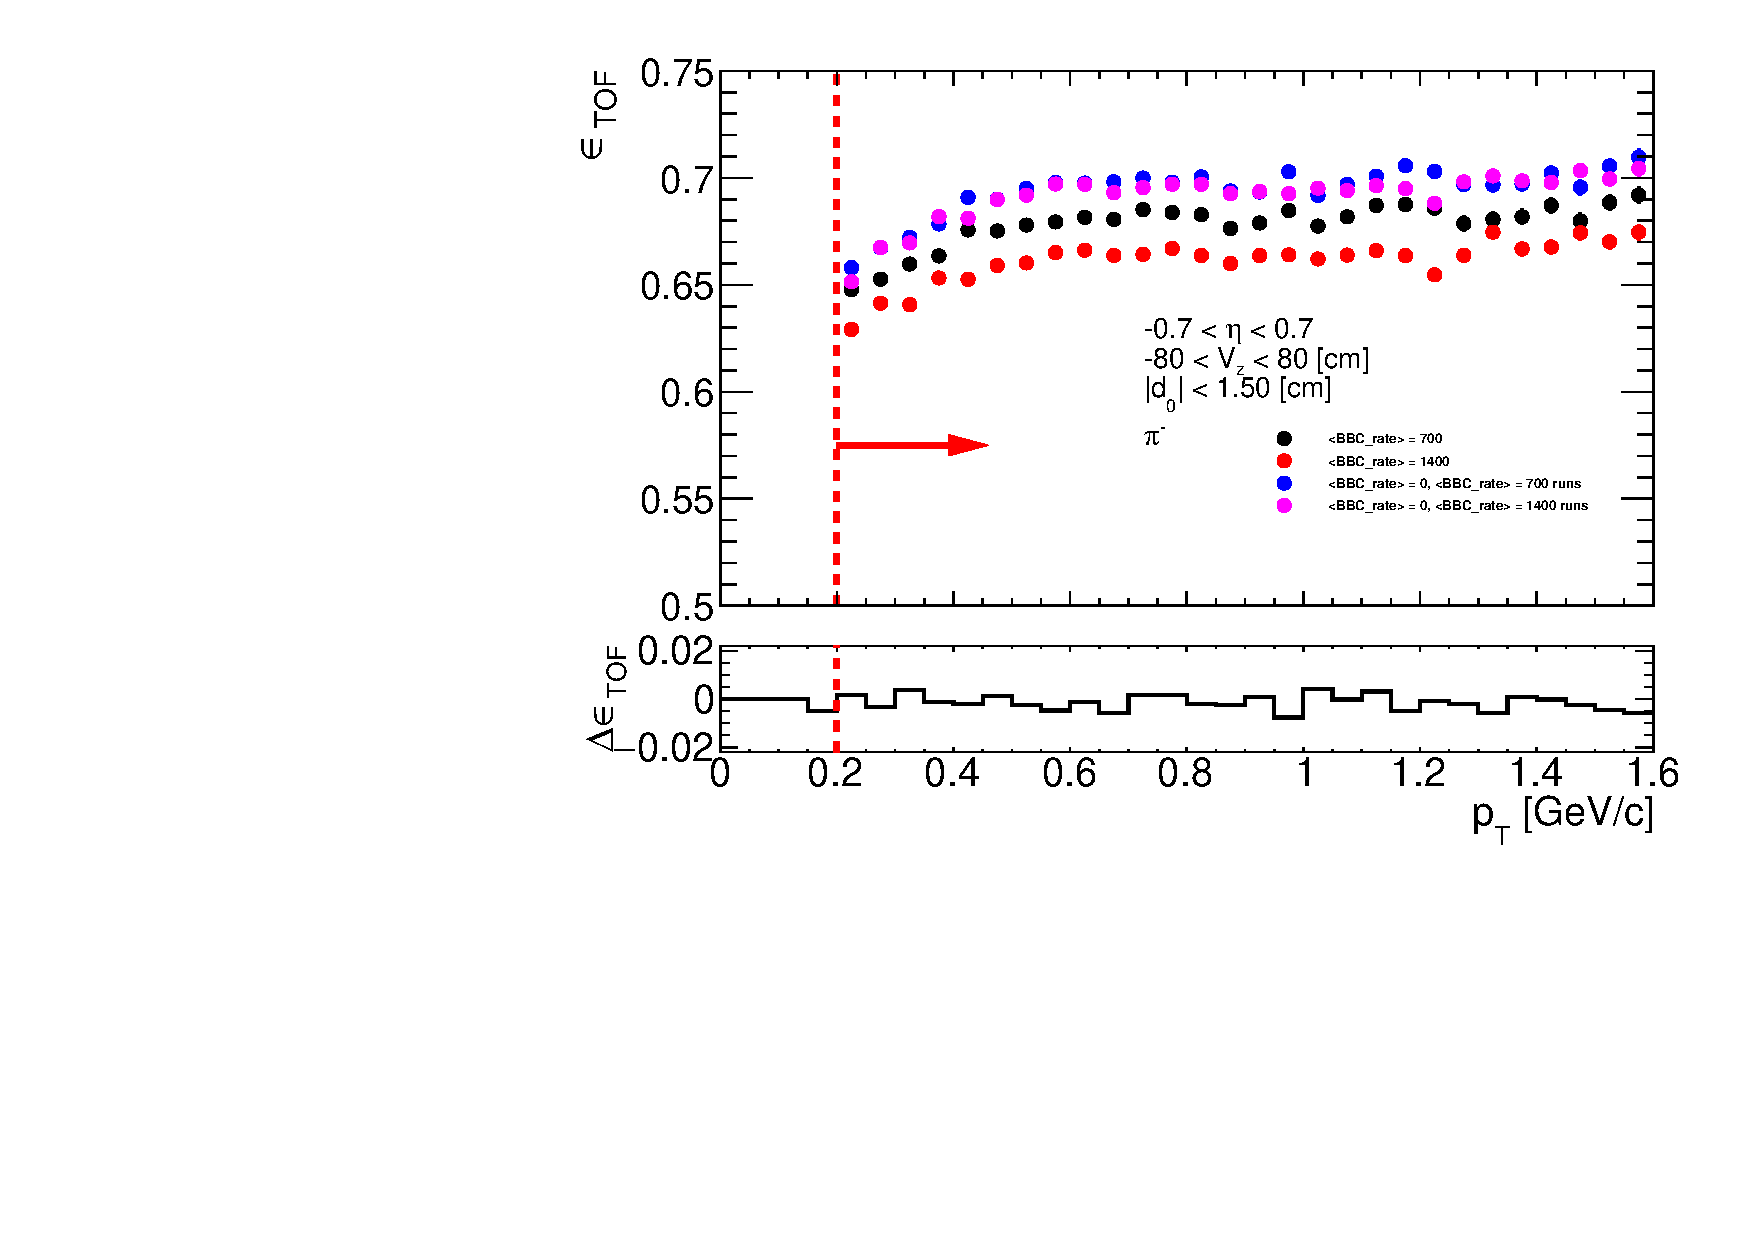
\includegraphics[width=\linewidth,page=1]{graphics/systematicsEfficiency/bbc_and/tofEffi_d0_1_5_etapt_1.pdf}\\
	}~
	\parbox{0.495\textwidth}{
		\centering
		\includegraphics[width=\linewidth,page=2]{graphics/systematicsEfficiency/bbc_and/tofEffi_d0_1_5_etapt_1.pdf}\\
	}%
	\caption[$\pi^\pm$ TOF matching efficiency as a function of $p_T$ $\left(|\eta|<0.7, |V_z|<80\text{ cm}\right)$ for embedded MC samples with \mbox{$<\text{BBC\_AND}>=700$~kHz} and \mbox{$<\text{BBC\_AND}>=1400$~kHz}]{$\pi^\pm$ TOF matching efficiency as a function of $p_T$ $\left(|\eta|<0.7, |V_z|<80\text{ cm}\right)$ for embedded MC samples with \mbox{$<\text{BBC\_AND}>=700$~kHz} and \mbox{$<\text{BBC\_AND}>=1400$~kHz}. The efficiences from corresponding no-pile-up MC samples were also shown. Additionally, the offset  from Eq. \ref{eq:tofSystDifference} was drawn in the bottom of each plot.}
	\label{fig:systError1Dtof}
\end{figure}
\begin{figure}[H]
	\centering
	\parbox{0.495\textwidth}{
		\centering
		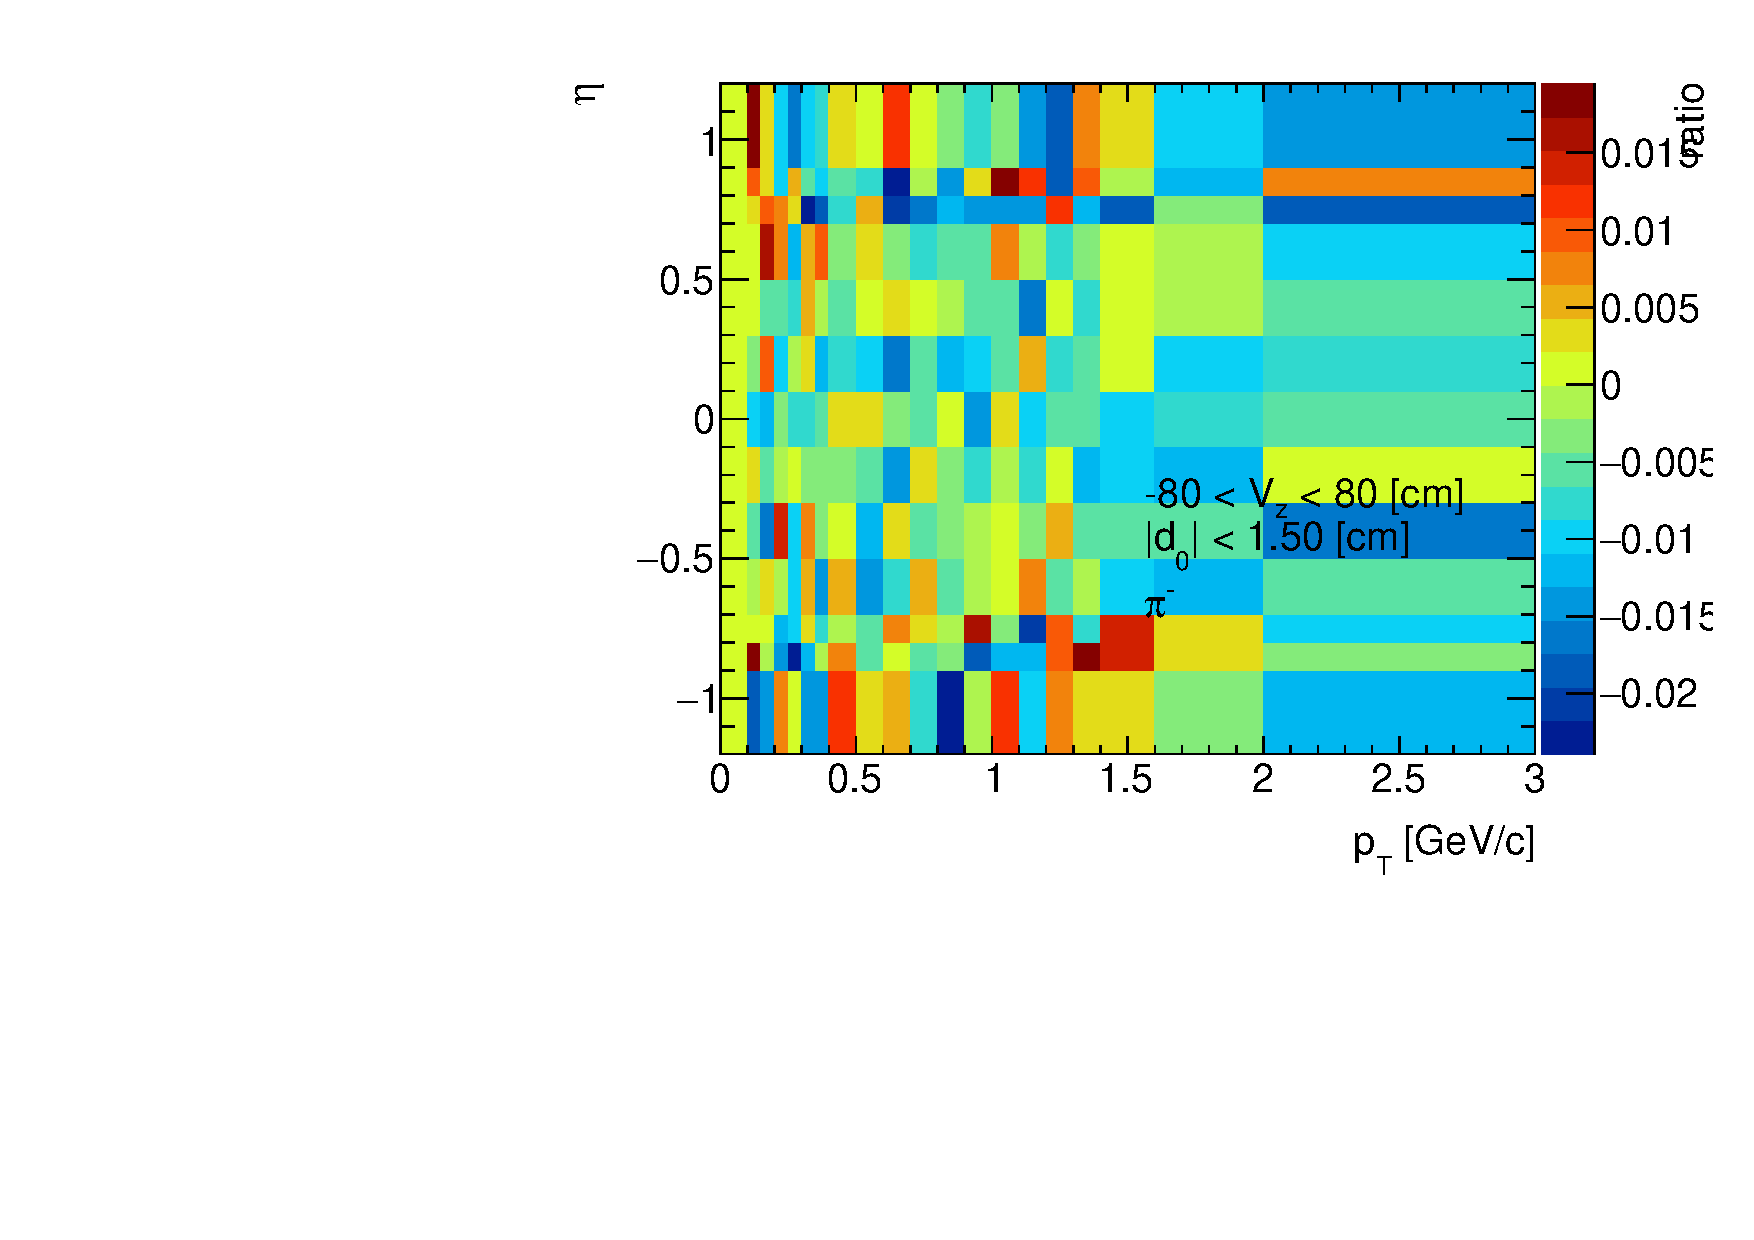
\includegraphics[width=\linewidth,page=1]{graphics/systematicsEfficiency/bbc_and/tofEffi_d0_1_5_etapt_12D.pdf}\\
	}~
	\parbox{0.495\textwidth}{
		\centering
		\includegraphics[width=\linewidth,page=2]{graphics/systematicsEfficiency/bbc_and/tofEffi_d0_1_5_etapt_12D.pdf}\\
	}%
	\caption[The difference $\Delta\epsilon_{ TOF} =\Delta\epsilon_{ TOF}^{1400\text{ kHz}}-2\cdot\Delta\epsilon_{ TOF}^{700\text{ kHz}}$ for $\pi^\pm$ as a function of $p_T$ and $\eta$ $\left(|V_z|<80\text{ cm}\right)$]{The offset $\Delta\epsilon_{ TOF} =\Delta\epsilon_{ TOF}^{1400\text{ kHz}}-2\cdot\Delta\epsilon_{ TOF}^{700\text{ kHz}}$ for $\pi^\pm$ as a function of $p_T$ and $\eta$ $\left(|V_z|<80\text{ cm}\right)$. }
	\label{fig:systError2Dtof}
\end{figure}



\subsection{TOF system simulation accuracy}\label{subsec:tofAbsEffSystAndCorr}

Systematic uncertainty of the TOF efficiency related to the accuracy of the TOF system simulation in STARsim and the data driven correction to it derived in Sec.~\ref{sec:tofAbsEffCorr} was estimated by comparing that nominal TOF efficiency with the one obtained with an independent method described below.

In some STAR analyses the TOF hit reconstruction and matching efficiency is determined from the data with the use of BEMC: real (in-time) tracks are selected based on the fact that they match to BEMC cluster. If they do, the TOF efficiency is calculated as a ratio of number of TOF-matched tracks to number of all tracks. This solution may provide slightly biased efficiency, because the signal in the detector placed behind TOF, such as BEMC, ensures that particle still followed the original helical path past the last hit of the track in TPC (Fig.~\ref{fig:hftEffSketch}). Also, BEMC clusters are more efficiently reconstructed as the energy deposits in the calorimeter increase, which may favor tracks which generated secondaries in front of the BEMC, hence possibly also in front of TOF thus increasing a chance to reconstruct hit in TOF.

To estimate systematic error of the TOF efficiency we decided to calculate efficiency utilizing the TPC tracks containing hits in HFT. The HFT is a group of silicon detectors (PXL, IST, SST) which differ from the gaseous detectors (like TPC) in many aspects. The difference that is most important for this study is the time of response/memory - much shorter in HFT than in TPC. Therefore if the TPC track contain hits in the silicon of HFT it is very probably a real track of particle produced in the proton-proton interaction in the corresponding bunch crossing. With this HFT-tagged tracks we ommit potential bias related to matching with BEMC cluster.

We used the data from st\_ssdmb stream (VPDMB-5-ssd trigger) from the same runs as the data used in our physics analyses. The HFT-tagged tracks were selected as the primary tracks passing the quality cuts \ref{sec:TpcQualityCuts} (only the TPC hits were counted). These tracks were required to contain hits in two HFT layers: IST ans SST, which vastly reduced probability to select an off-time track in TPC (PXL was not used in reconstruction due to problems in firmware). As shown in Fig.~\ref{fig:zVtxHFT}, the $z_{\text{vtx}}$ coverage of the HFT-tagged tracks is limited to about $\pm20$~cm. We imposes cut on the $z$ position of the vertex $|z_{\text{\text{vtx}}}|<20$~cm to remove tracks from the tails, which generally have large $|\eta|$.

Identification of particles was done using the specific energy loss measured in the TPC ($n^{\sigma}$ variables were used). The following requirements were imposed on $n^{\sigma}$ variables in order to select three species of particles whose tracks were selected for the TOF efficiency analysis:
\begin{itemize}
 \item pions:~~~~~$|n^{\sigma}_{\text{pion}}| < 2$,
 \item kaons:~~~~~$-2 < n^{\sigma}_{\text{proton}} < 2.5$~~~\&\&~~~$|n^{\sigma}_{\text{pion}}| > 3.5$~~~\&\&~~~$|n^{\sigma}_{\text{electron}}| > 3.5$~~~\&\&~~~$|n^{\sigma}_{\text{proton}}| > 3.5$,
 \item protons:~~$-2 < n^{\sigma}_{\text{proton}} < 3$~~~~~\&\&~~~~$|n^{\sigma}_{\text{pion}}| > 3.5$~~~\&\&~~~$|n^{\sigma}_{\text{electron}}| > 3.5$~~~\&\&~~~$|n^{\sigma}_{\text{kaon}}| > 3.5$.
\end{itemize}

%---------------------------
\begin{figure}[b!]%\vspace{-2pt}%
\centering%
\begin{minipage}{.4725\textwidth}%
  \centering%\vspace{11pt}
  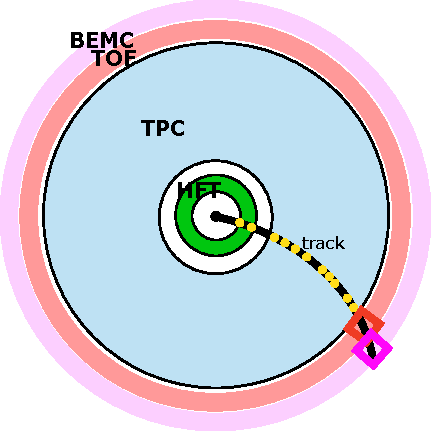
\includegraphics[width=0.965\linewidth]{graphics/systematicsEfficiency/TofSyst/effSketch.pdf}%\vspace{-5pt}%
  \caption[Sketch of the track with points in HFT.]%
  {Sketch of the cross section of the central detector and the track reconstructed with points in HFT. Presence of HFT points in a reconstructed track can be used as a tagger of the in-time tracks.}
  \label{fig:hftEffSketch}
\end{minipage}%
\quad\quad%
\begin{minipage}{.4725\textwidth}%
  \centering%
  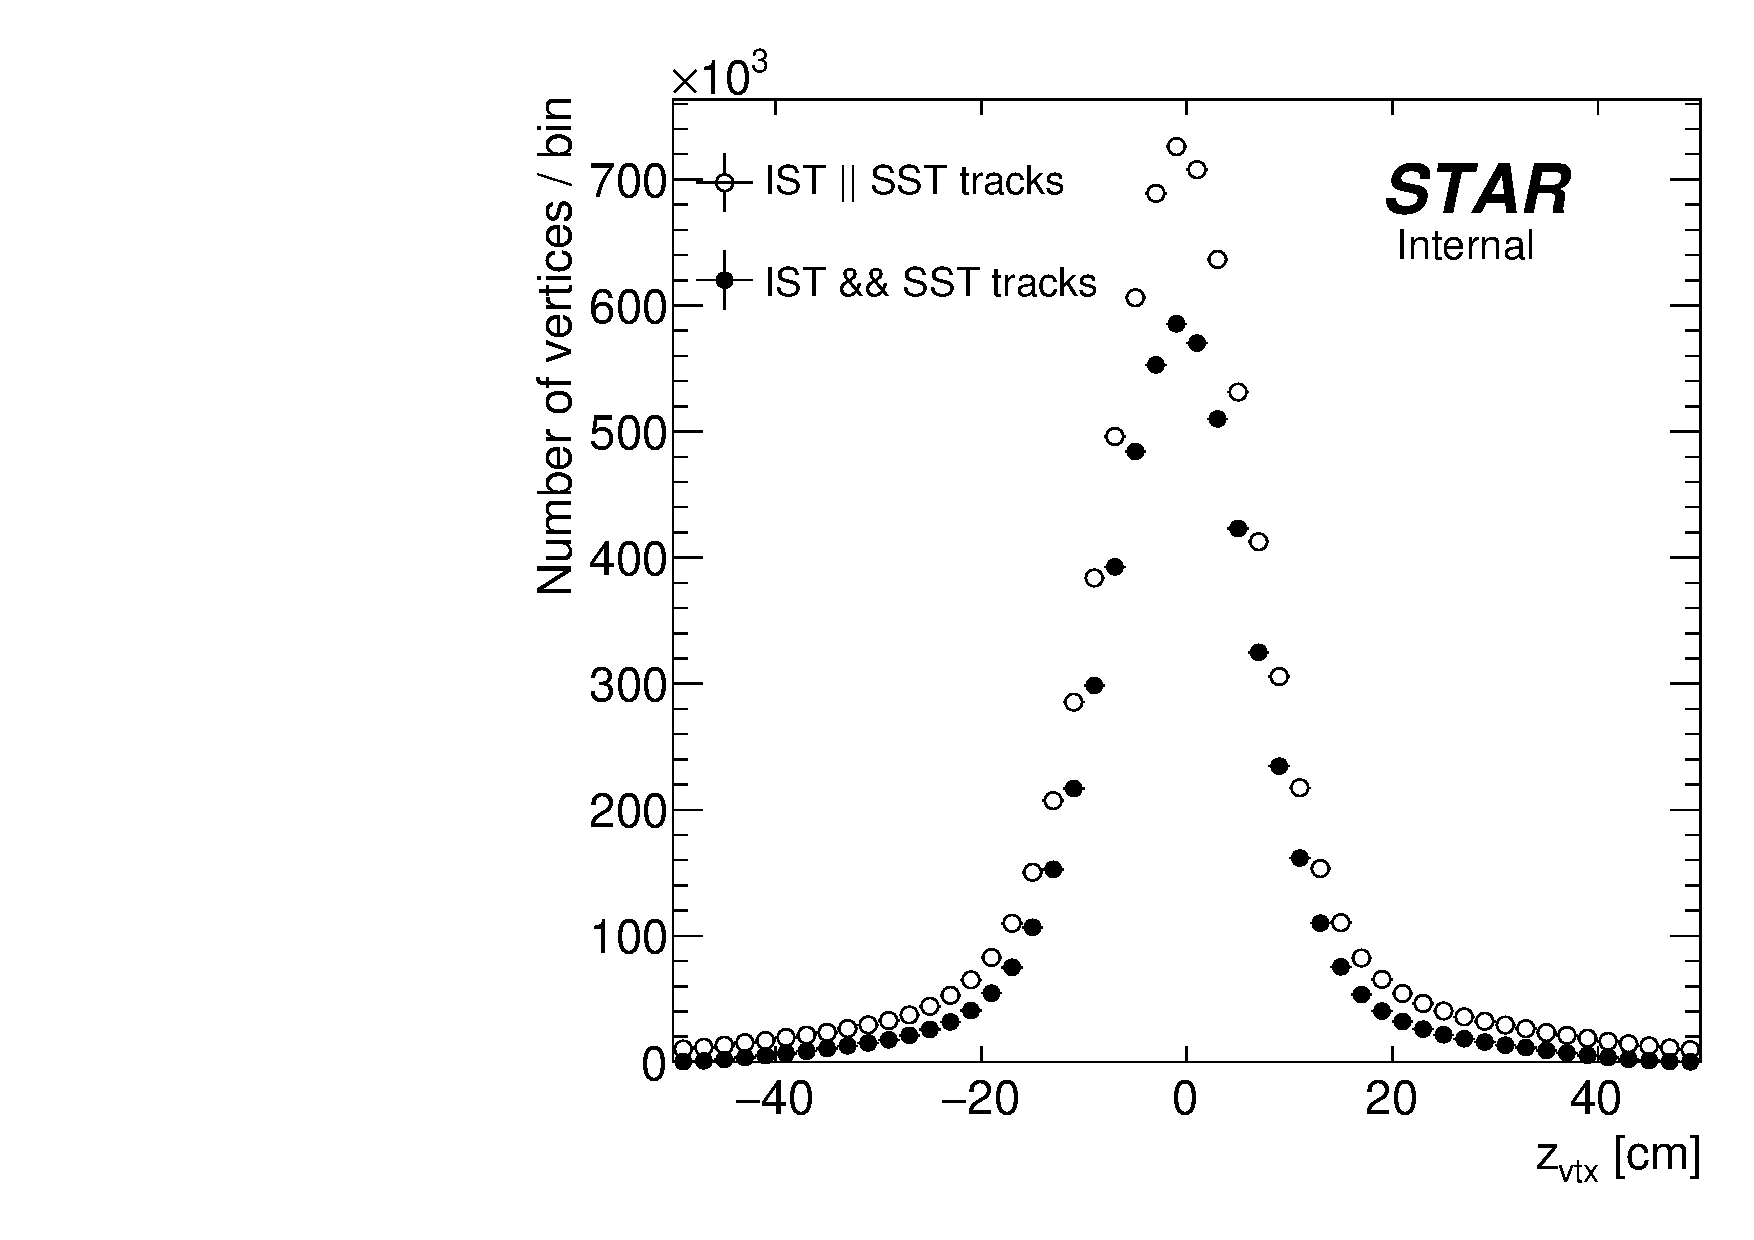
\includegraphics[width=\linewidth]{graphics/systematicsEfficiency/TofSyst/zVtxHFT.pdf}%\vspace*{-5pt}
  \caption[Distribution of $z$-position of vertices with TPC tracks containing hits in HFT.]
   {Distribution of $z$-position of vertices containing TPC tracks with HFT hits (st\_ssd stream). Open circles represent vertices with tracks with hits in IST or SST, full circles - IST and SST.}
   \label{fig:zVtxHFT}%\vspace*{-29pt} 
\end{minipage}%
\end{figure}%
%---------------------------  

\noindent Selection of pions by cut solely on $n^{\sigma}_{\text{pion}}$ (without additional cuts on $n^{\sigma}$ for kaon, proton and electron hypothesis) is driven by the dominance of pion production over other species and by the fact that the dE/dx of pions overlap with kaons and protons at momenta which are relatively large, hence the TOF efficiency is saturated and the same for all particle species. More sophisticated selection was used for kaons and protons. Figure~\ref{fig:hftTracksNSigmaVsPt} shows the $n^{\sigma}$ variables before and after the selection of kaons (\ref{fig:hftTracksNSigmaKaonVsPt}) and protons (\ref{fig:hftTracksNSigmaProtonVsPt}), where one can find proof that clean samples of these particles were selected, for the price of limited coverage in track $p_{T}$.
%---------------------------
\begin{figure}[t!]
\centering
\parbox{0.4725\textwidth}{
  \centering
  \begin{subfigure}[b]{\linewidth}
                \subcaptionbox{\label{fig:hftTracksNSigmaKaonVsPt}}{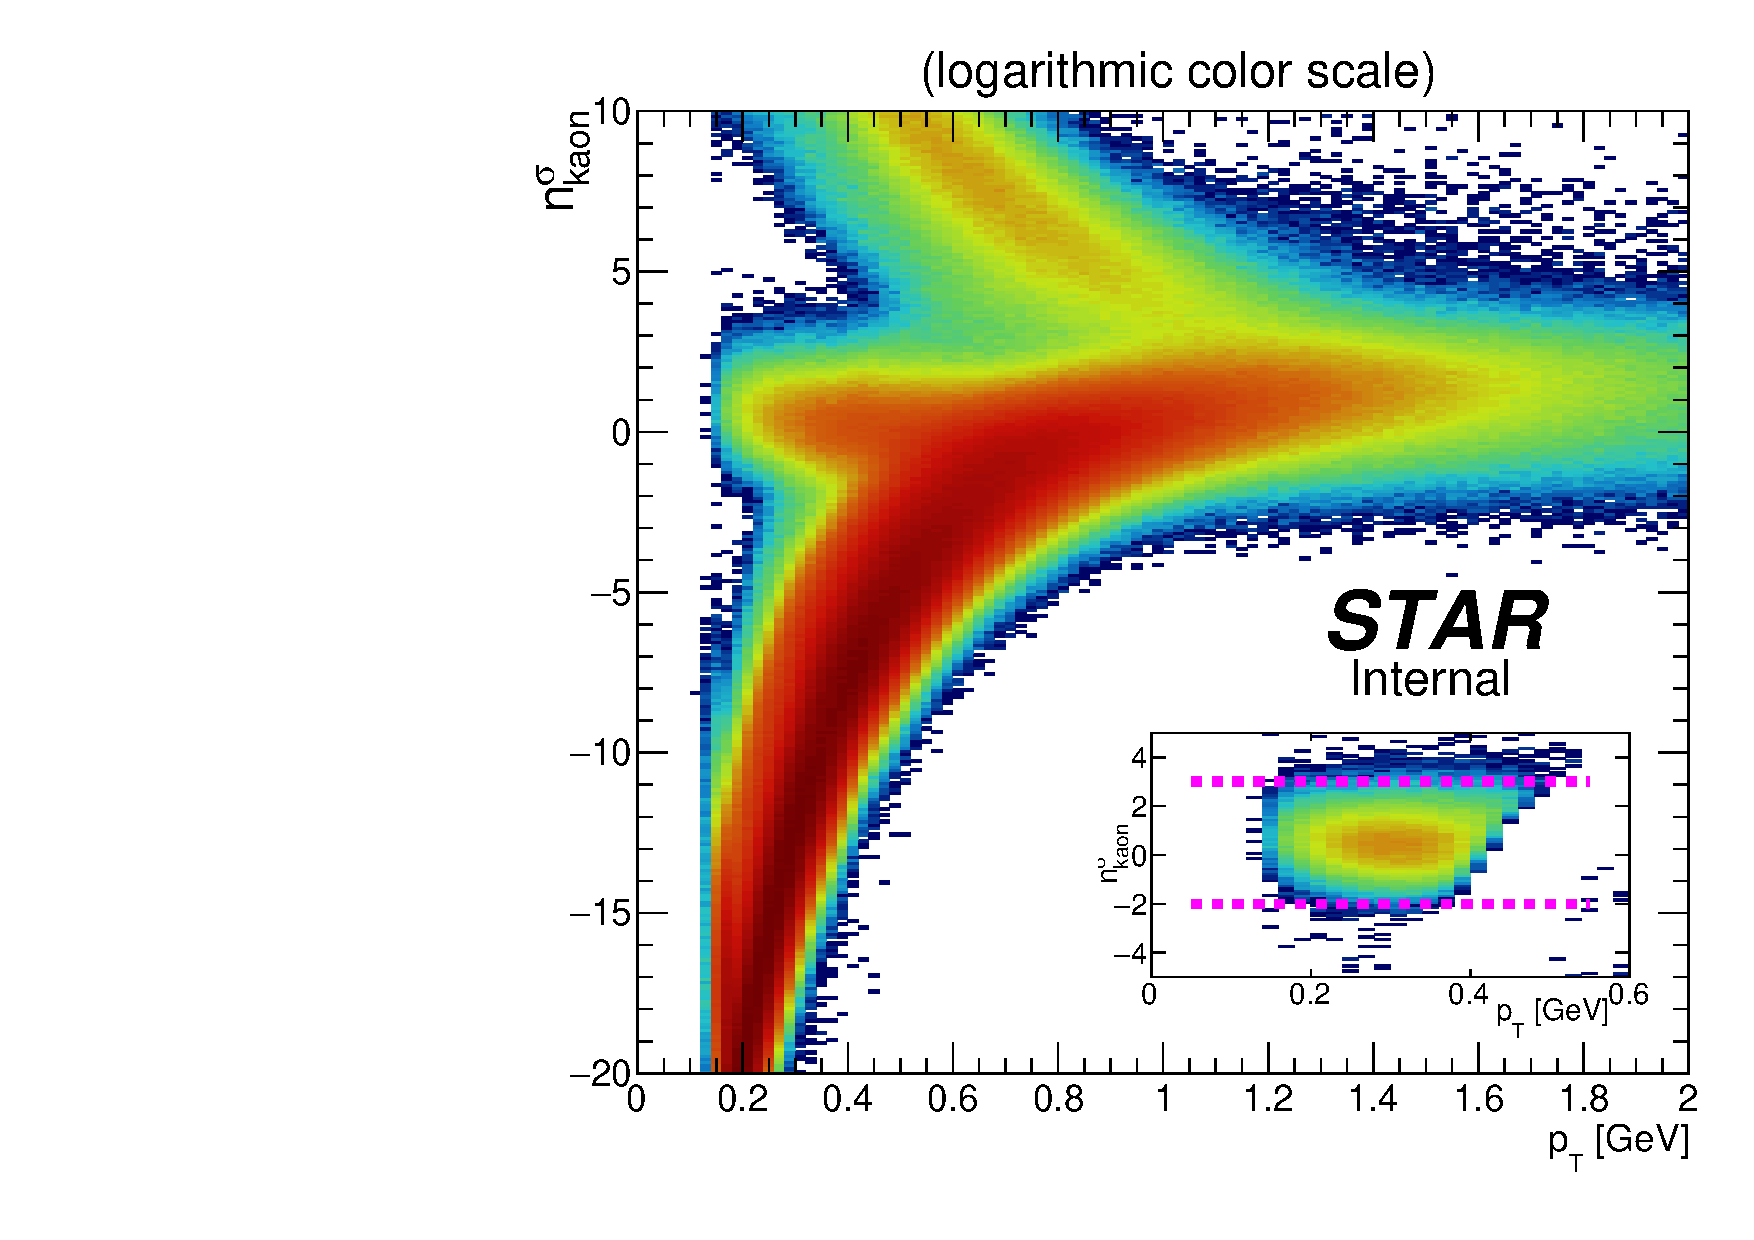
\includegraphics[width=\linewidth]{graphics/systematicsEfficiency/TofSyst/NSigmaKaonVsPt.pdf}\vspace{-10pt}}\vspace{-5pt}
  \end{subfigure}
}%
\quad\quad%
\parbox{0.4725\textwidth}{
  \centering
  \begin{subfigure}[b]{\linewidth}
                \subcaptionbox{\label{fig:hftTracksNSigmaProtonVsPt}}{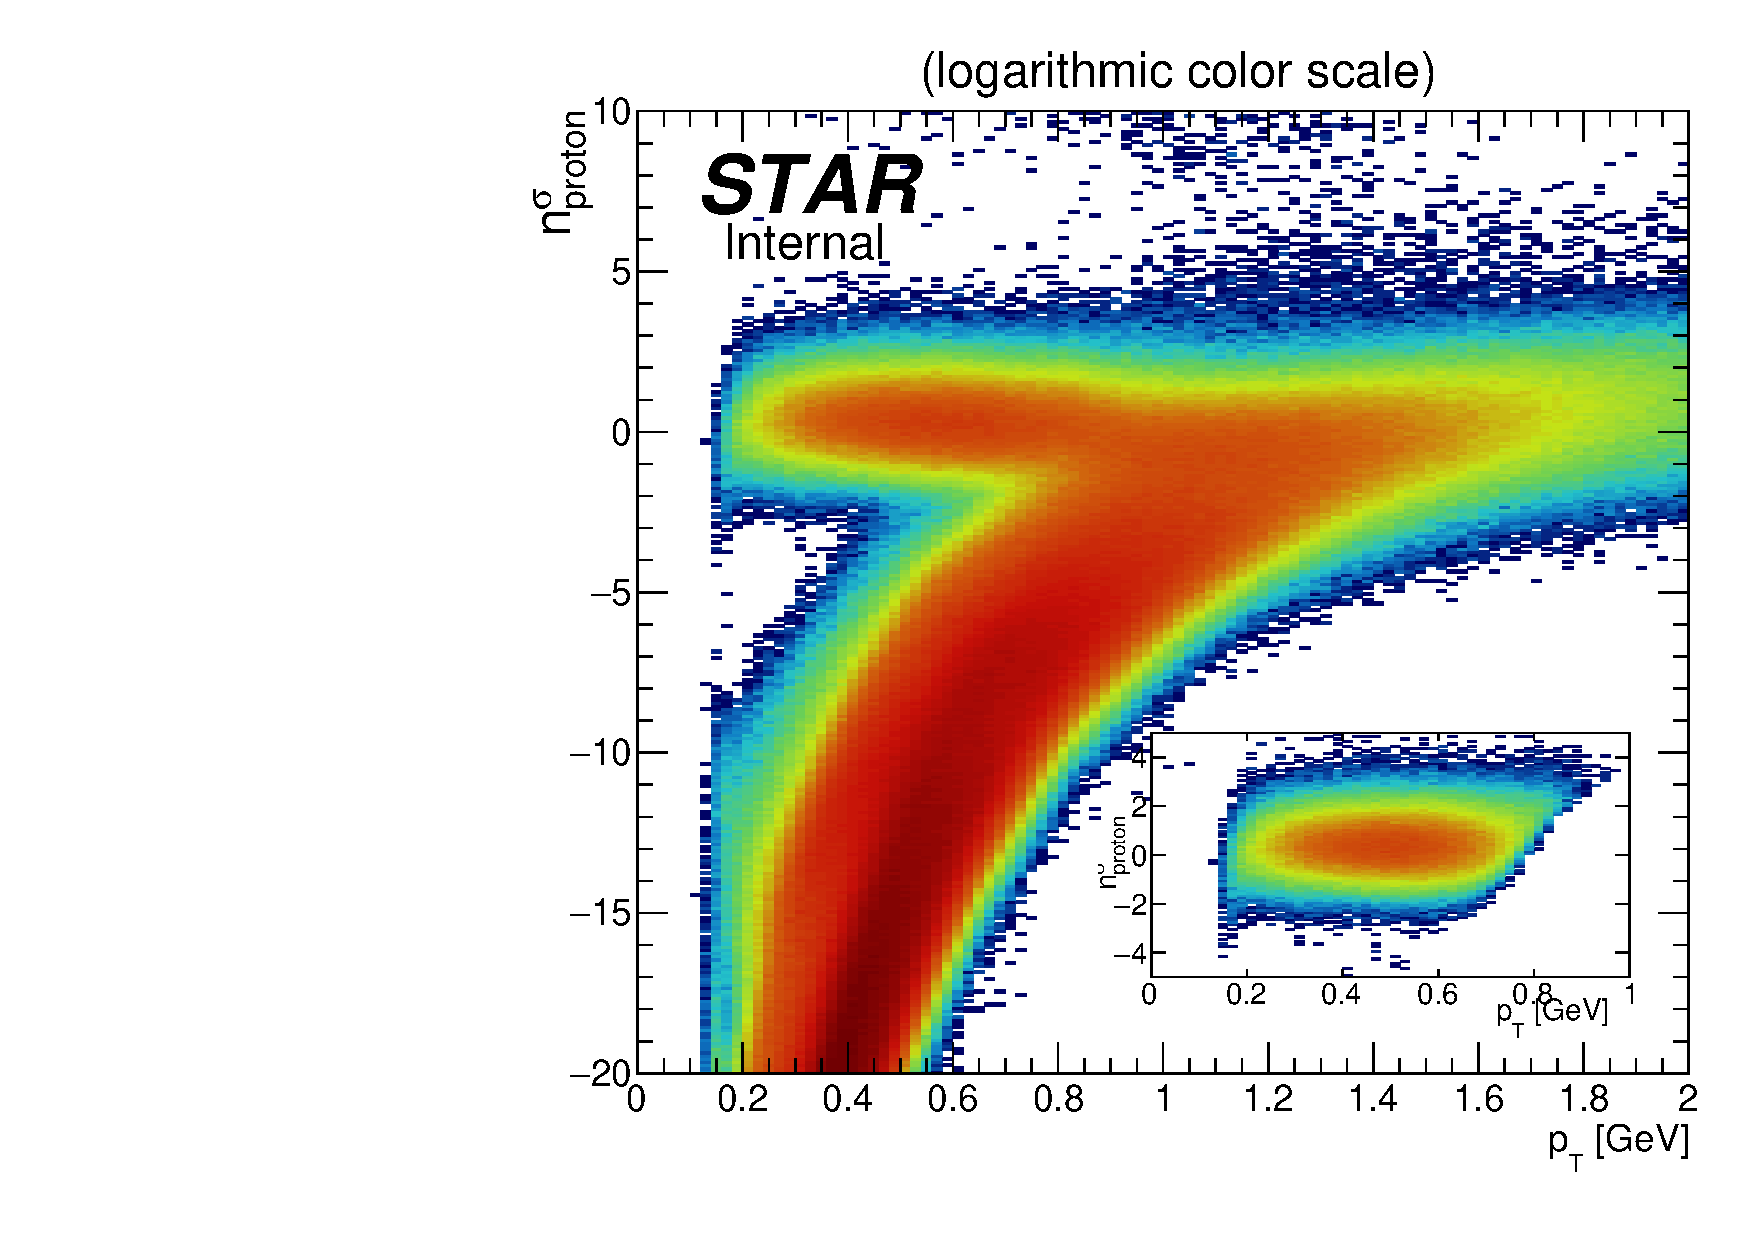
\includegraphics[width=\linewidth]{graphics/systematicsEfficiency/TofSyst/NSigmaProtonVsPt.pdf}\vspace{-10pt}}\vspace{-5pt}
  \end{subfigure}
}%
\caption[Distribution of $n^{\sigma}$ (kaon and proton) vs. transverse momentum for tracks containing HFT hits.]%
    {Distribution of $n^{\sigma}_{\text{kaon}}$ (\ref{fig:hftTracksNSigmaKaonVsPt}) and $n^{\sigma}_{\text{proton}}$ (\ref{fig:hftTracksNSigmaProtonVsPt}) vs. track $p_{T}$ for tracks containing HFT hits. The insert in each subfigure shows the corresponding $n^{\sigma}$ vs. $p_{T}$ distribution after preselection of tracks of given spiecies (without cut on variable in $y$-axis) according to description provided in the text in preceding page. Dashed magenta lines represent final cuts on corresponding $n^{\sigma}$ quantity used to select tracks of given species.}\label{fig:hftTracksNSigmaVsPt}%
\end{figure}
%---------------------------

%---------------------------
\begin{figure}[b!]\vspace{-34pt}
\centering
\parbox{0.31\textwidth}{
  \centering
  \begin{subfigure}[b]{\linewidth}{
                \subcaptionbox{\label{fig:TPcorrectionTofEff2D}}{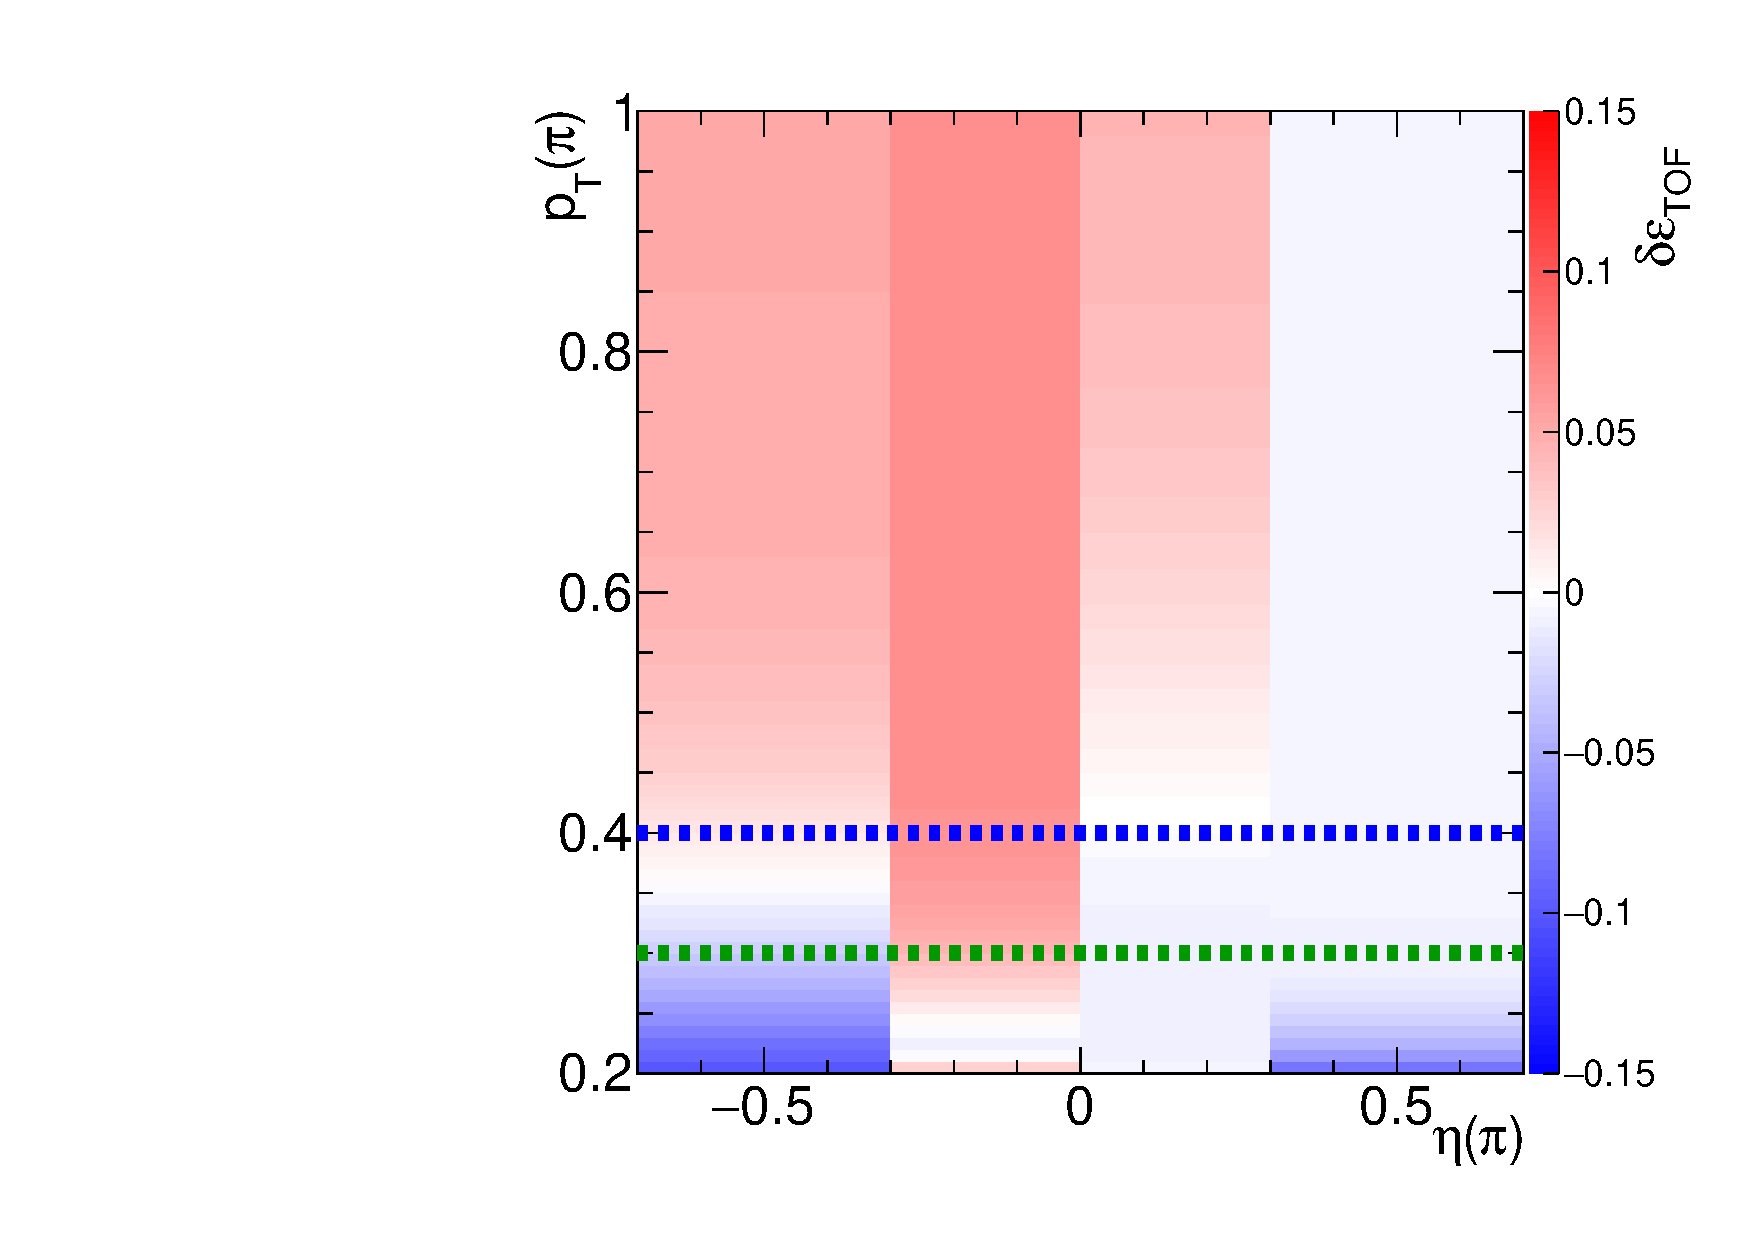
\includegraphics[width=\linewidth]{graphics/systematicsEfficiency/TofSyst/TofEffCorrection2D_pion.pdf}\vspace{-12pt}}}
  \end{subfigure} 
} 
\quad
\parbox{0.65\textwidth}{ 
  \centering
		\begin{minipage}[t][0.64\linewidth][t]{\linewidth}\vspace{73pt}
			\caption[Comparison of the TOF eff. correction from tag\&probe method and the difference between TOF eff. calculated using standard method from the HFT-tagged tracks and efficiency from embedded single particle MC.]%
    {Comparison of the TOF efficiency correction obtained with tag\&probe method on CEP $\pi^{+}\pi^{-}$ events (\ref{fig:TPcorrectionTofEff2D}, description in Sec.~\ref{sec:tofAbsEffCorr}) and the difference between TOF efficiency calculated using standard method from the HFT-tagged tracks and efficiency from embedded single particle MC for pions (\ref{fig:tofEffDifference_pion}), kaons (\ref{fig:tofEffDifference_kaon}) and protons (\ref{fig:tofEffDifference_proton}). Yellow hatched area mark empty bins. Dashed horizontal lines represent minimum track $p_{T}$ thresholds used in our analyses: $0.3$~GeV for kaons (green) and $0.4$~GeV for protons (blue).}\label{fig:tofEffSystematics2DComparison}% 
		\end{minipage}
}\\[-25pt]
\parbox{0.31\textwidth}{
  \centering
  \begin{subfigure}[b]{\linewidth}{
                \subcaptionbox{\label{fig:tofEffDifference_pion}}{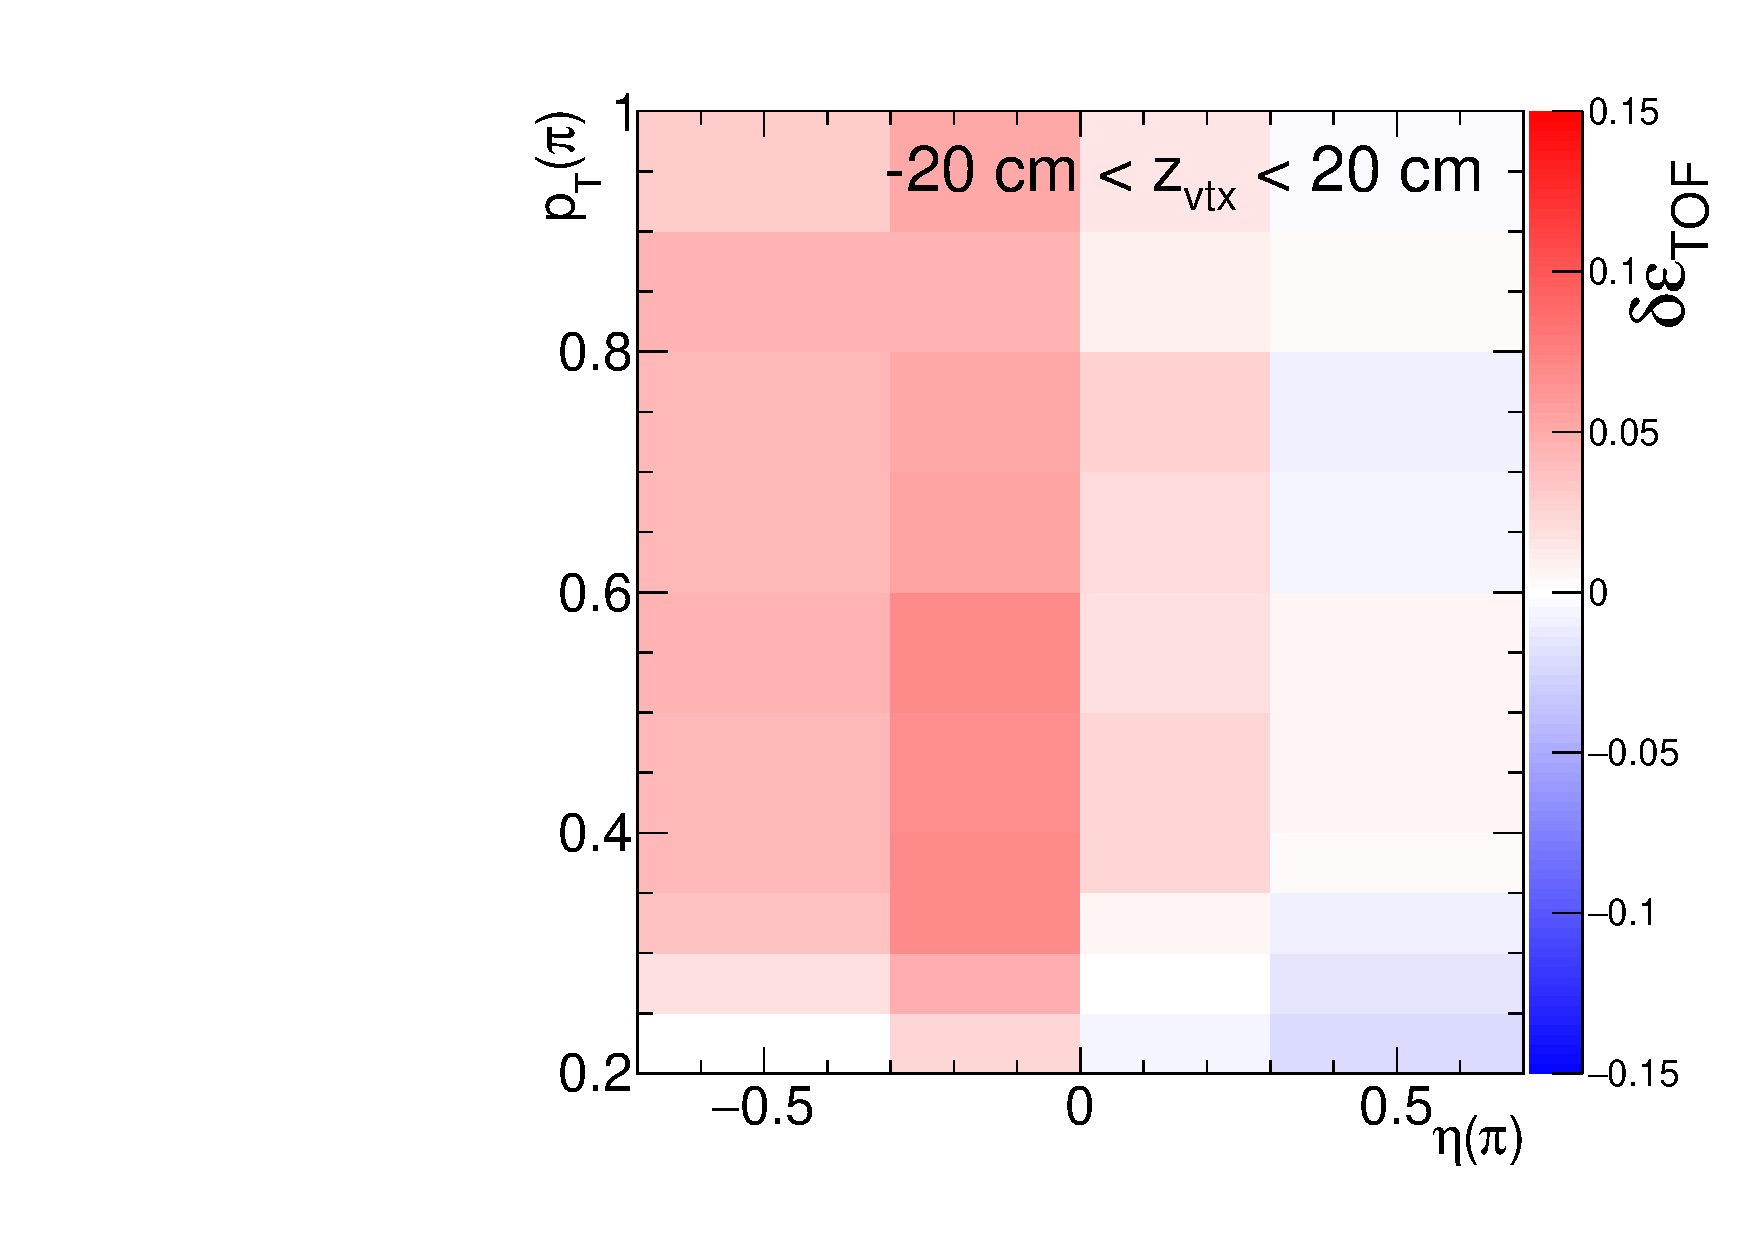
\includegraphics[width=\linewidth]{graphics/systematicsEfficiency/TofSyst/tofEffDifference_pion.pdf}\vspace{-12pt}}}
  \end{subfigure}
}
\quad
\parbox{0.31\textwidth}{
  \centering
  \begin{subfigure}[b]{\linewidth}{
                \subcaptionbox{\label{fig:tofEffDifference_kaon}}{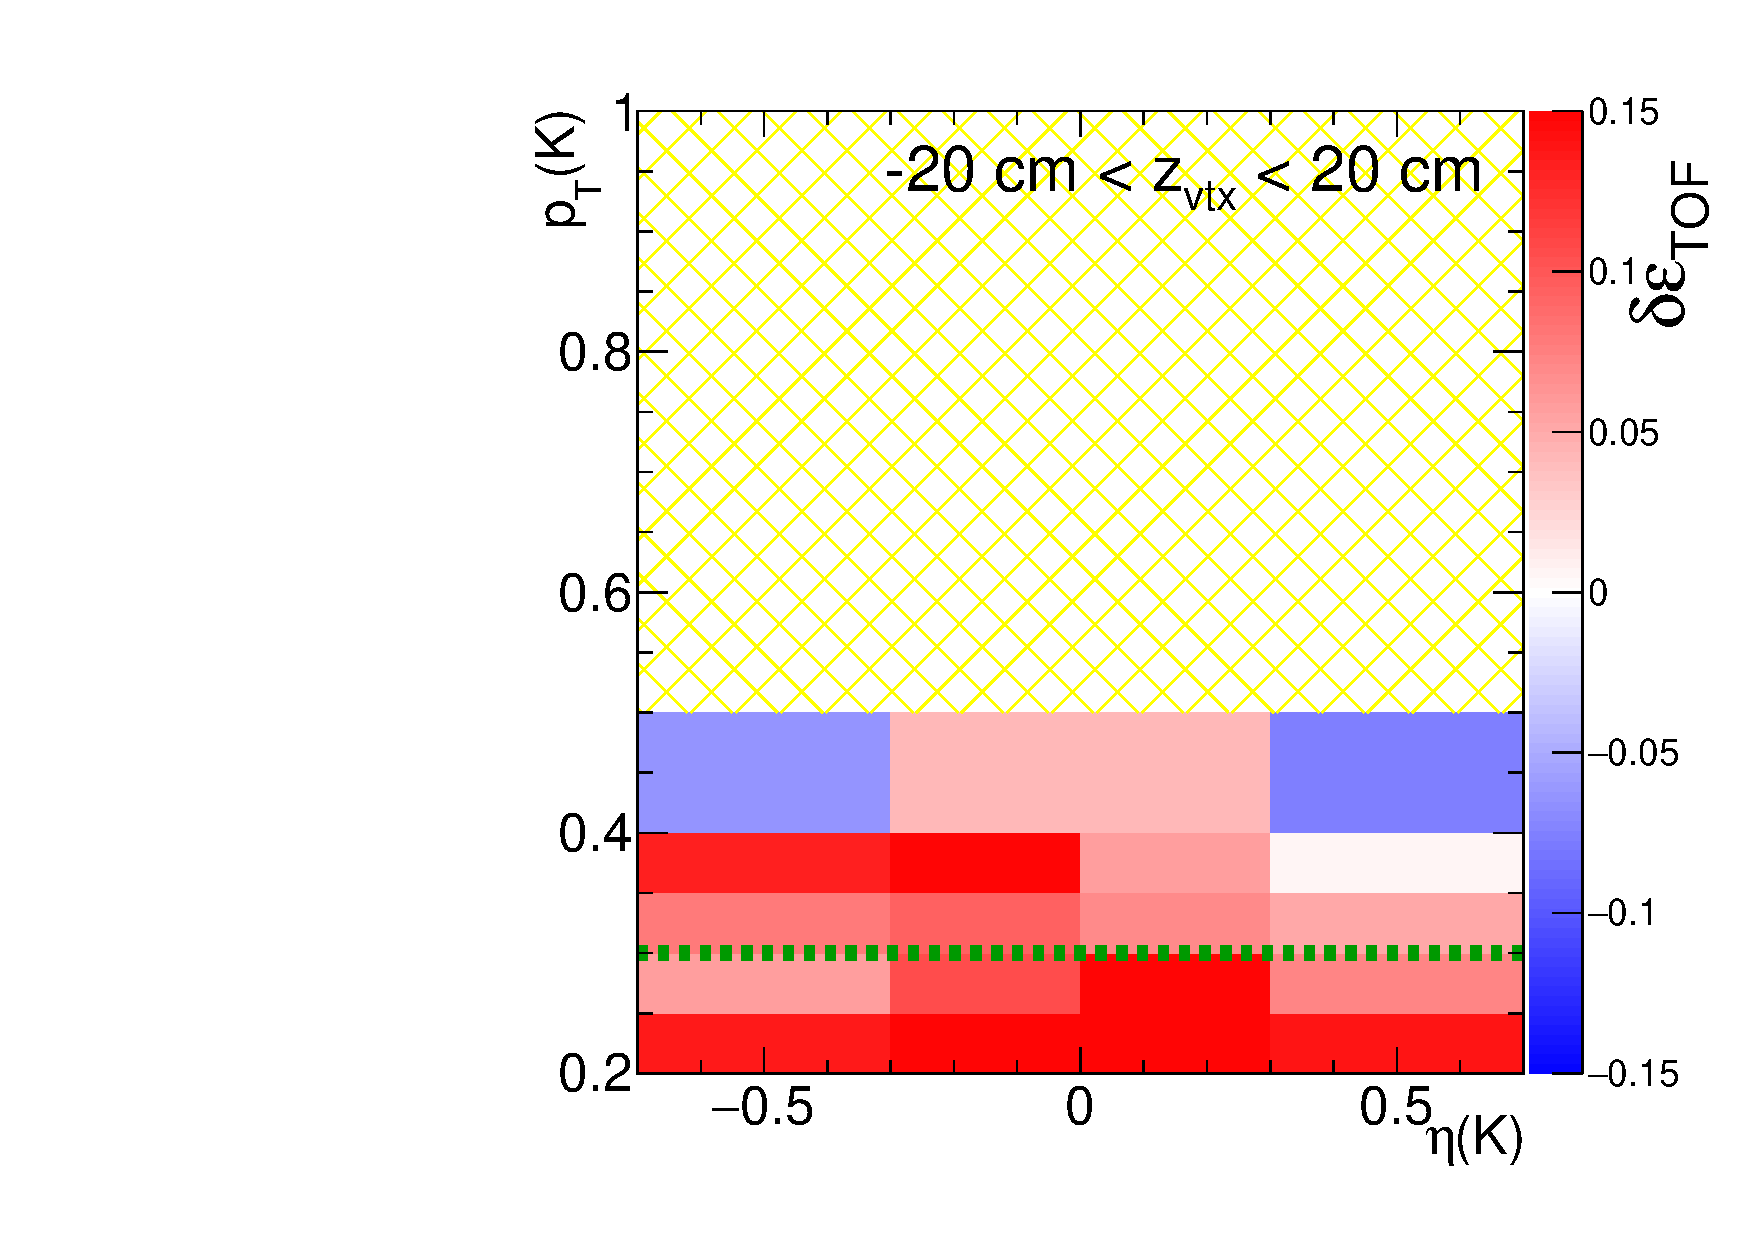
\includegraphics[width=\linewidth]{graphics/systematicsEfficiency/TofSyst/tofEffDifference_kaon.pdf}\vspace{-12pt}}}
  \end{subfigure}
} 
\quad
\parbox{0.31\textwidth}{
  \centering
  \begin{subfigure}[b]{\linewidth}{
                \subcaptionbox{\label{fig:tofEffDifference_proton}}{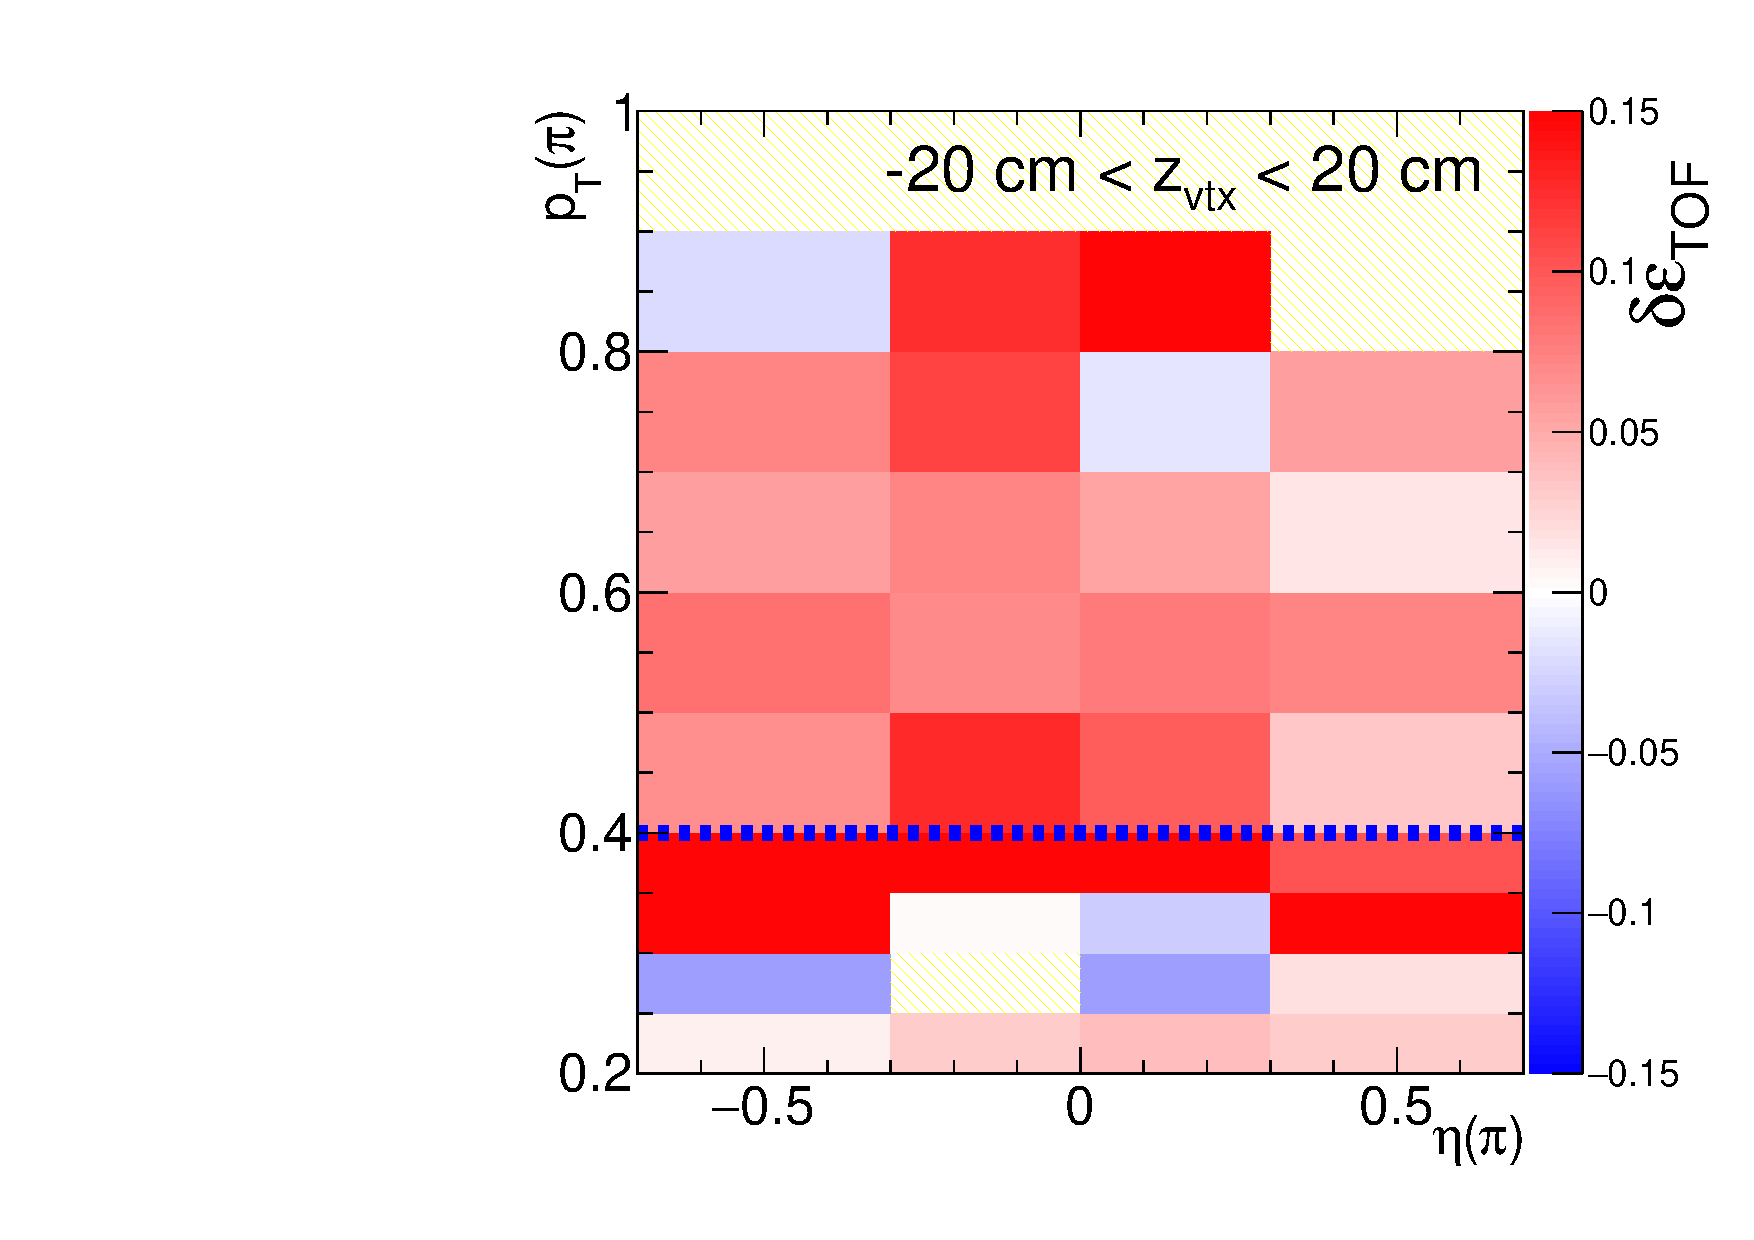
\includegraphics[width=\linewidth]{graphics/systematicsEfficiency/TofSyst/tofEffDifference_proton.pdf}\vspace{-12pt}}}
  \end{subfigure}
}

\end{figure}
%---------------------------


From selected sample of pion, kaon and proton tracks the TOF hit reconstruction and matching efficiency was calculated using the standard method - as a ratio of number of tracks matched with TOF and number of all tracks. This efficiency was compared with the efficiency extracted from the zero-bias-embedded single particle MC, calculated for $|z_{\text{vtx}}|<20$~cm and averaged between positive- and negative-charge particles. The result of comparison - the difference between efficiency calculated with HFT-tagged tracks and efficiency from single particle MC, is presented in Fig.~\ref{fig:tofEffSystematics2DComparison} (subfigures \ref{fig:tofEffDifference_pion}-\ref{fig:tofEffDifference_proton}). This difference could be interpreted as a data-driven correction to the TOF efficiency calculated from single particle MC, alternative to correction derived with tag\&probe method on CEP events, described in Sec.~\ref{sec:tofAbsEffCorr}.

The difference between an alternative correction in Figs.~\ref{fig:tofEffDifference_pion}-\ref{fig:tofEffDifference_proton} and the correction from tag\&probe (Fig.\ref{fig:TPcorrectionTofEff2D}) method, $\Delta\delta\varepsilon_{\text{TOF}}$, can be used as a measure of the uncertainty of the overall TOF efficiency. Aforementioned difference is depicted in Fig.~\ref{fig:tofEffDifference_Delta}. We decided to symmetrize the systematic uncertainty of the TOF efficiency. For this purpose, on top of the correction to the TOF efficiency from CEP tag\&probe method, we add the half of the difference from Fig.~\ref{fig:tofEffDifference_Delta} to the TOF efficiency of corresponding particle type. We then assign a systematic uncertainty of the TOF efficiency to each $(\eta,p_{T})$ bin as an absolute value of the half of that difference, $\frac{1}{2}|\Delta\delta\varepsilon_{\text{TOF}}|$. We assume that the systematic uncertainty for tracks whose $|z_{\text{vtx}}|>20$~cm is the same as for HFT tracks studied here ($|z_{\text{vtx}}|<20$~cm). For high track $p_{T}$, when there are no estimates of $\Delta\delta\varepsilon_{\text{TOF}}$, the average value from the 2 last non-empty $p_{T}$ bin (at given $\eta$ bin) is used as a correction, and maximum absolute value among the last 3 non-empty $p_{T}$ bins (at given $\eta$ bin) is used as a systematic uncertainty.

%---------------------------
\begin{figure}[h]%\vspace{-38pt} 
\centering
\parbox{0.31\textwidth}{
  \centering
  \begin{subfigure}[b]{\linewidth}{
                \subcaptionbox{\label{fig:tofEffDifference_Delta_pion}}{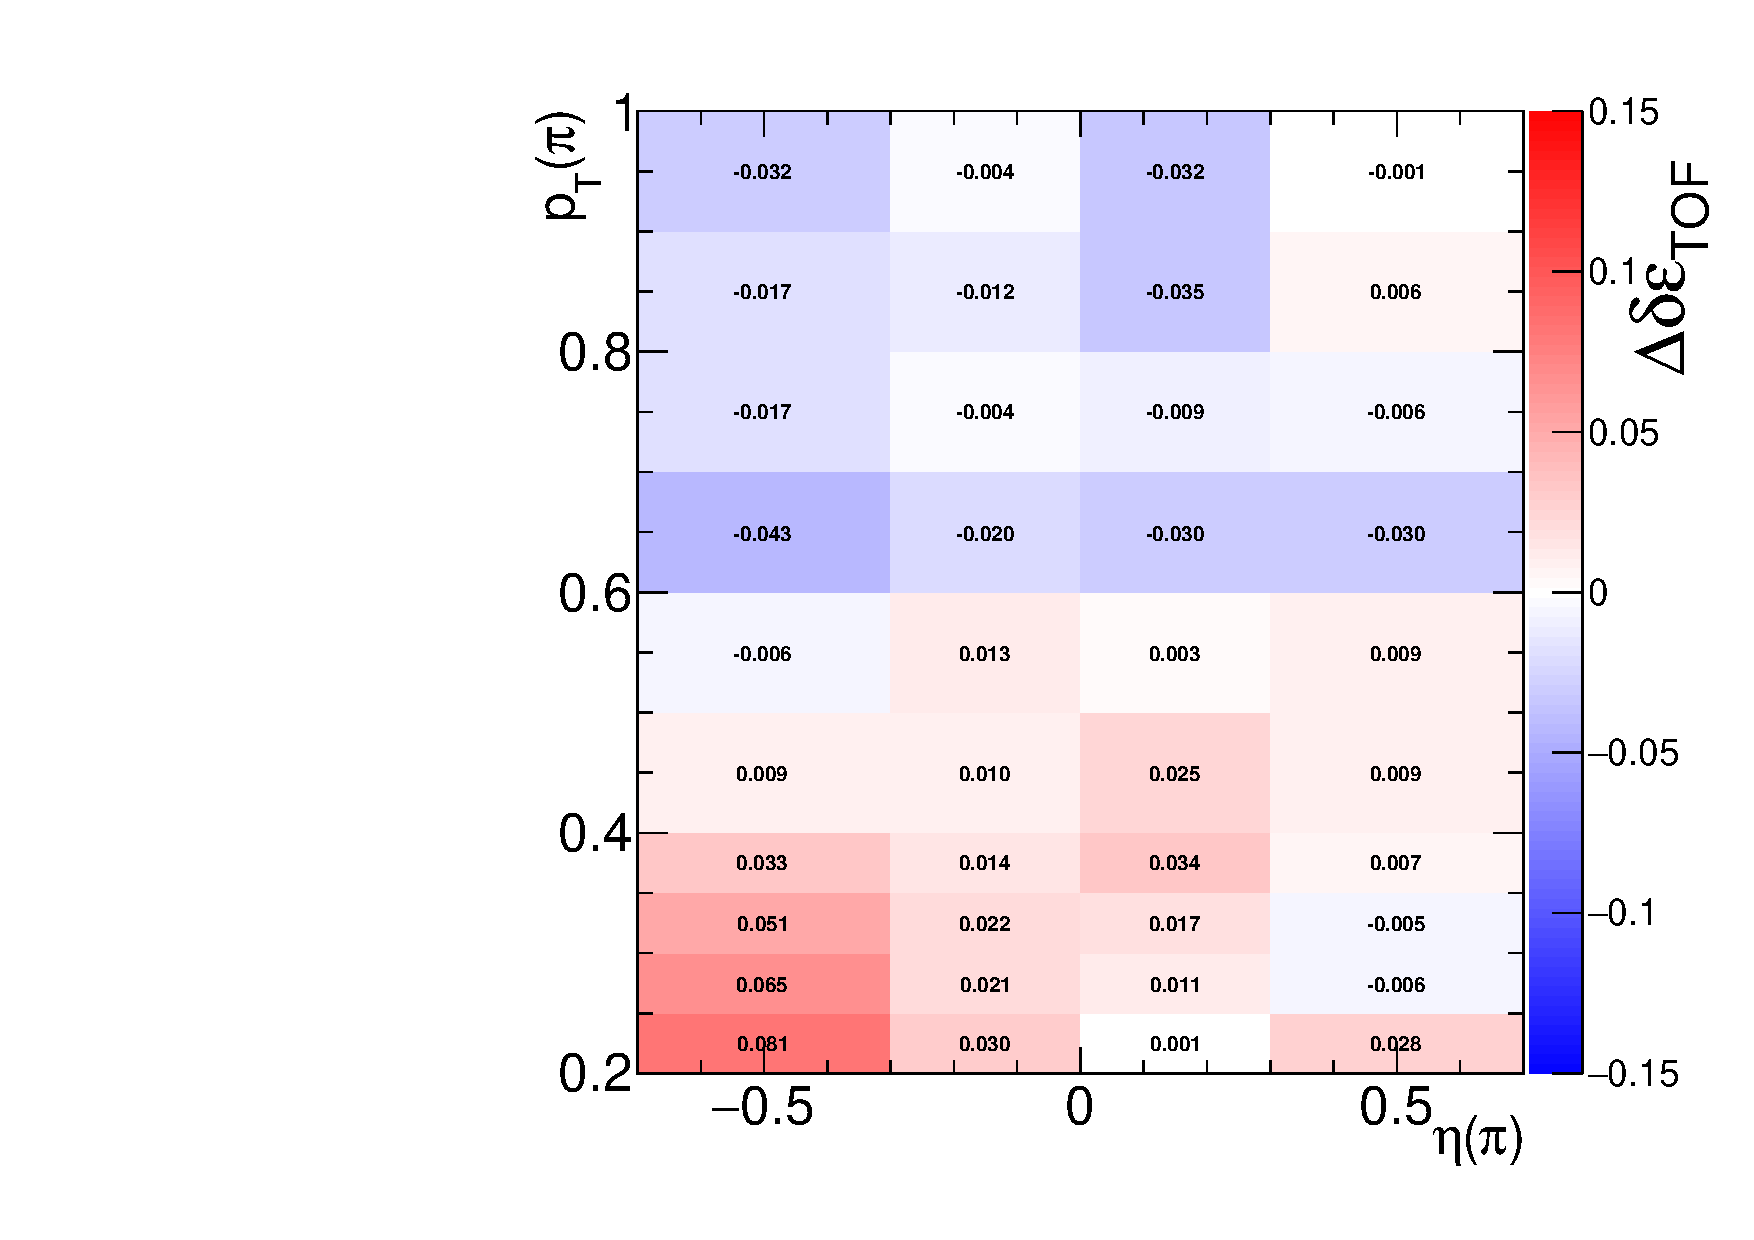
\includegraphics[width=\linewidth]{graphics/systematicsEfficiency/TofSyst/tofEffDifference_Delta_pion.pdf}\vspace{-12pt}}}
  \end{subfigure}
}
\quad
\parbox{0.31\textwidth}{
  \centering
  \begin{subfigure}[b]{\linewidth}{
                \subcaptionbox{\label{fig:tofEffDifference_Delta_kaon}}{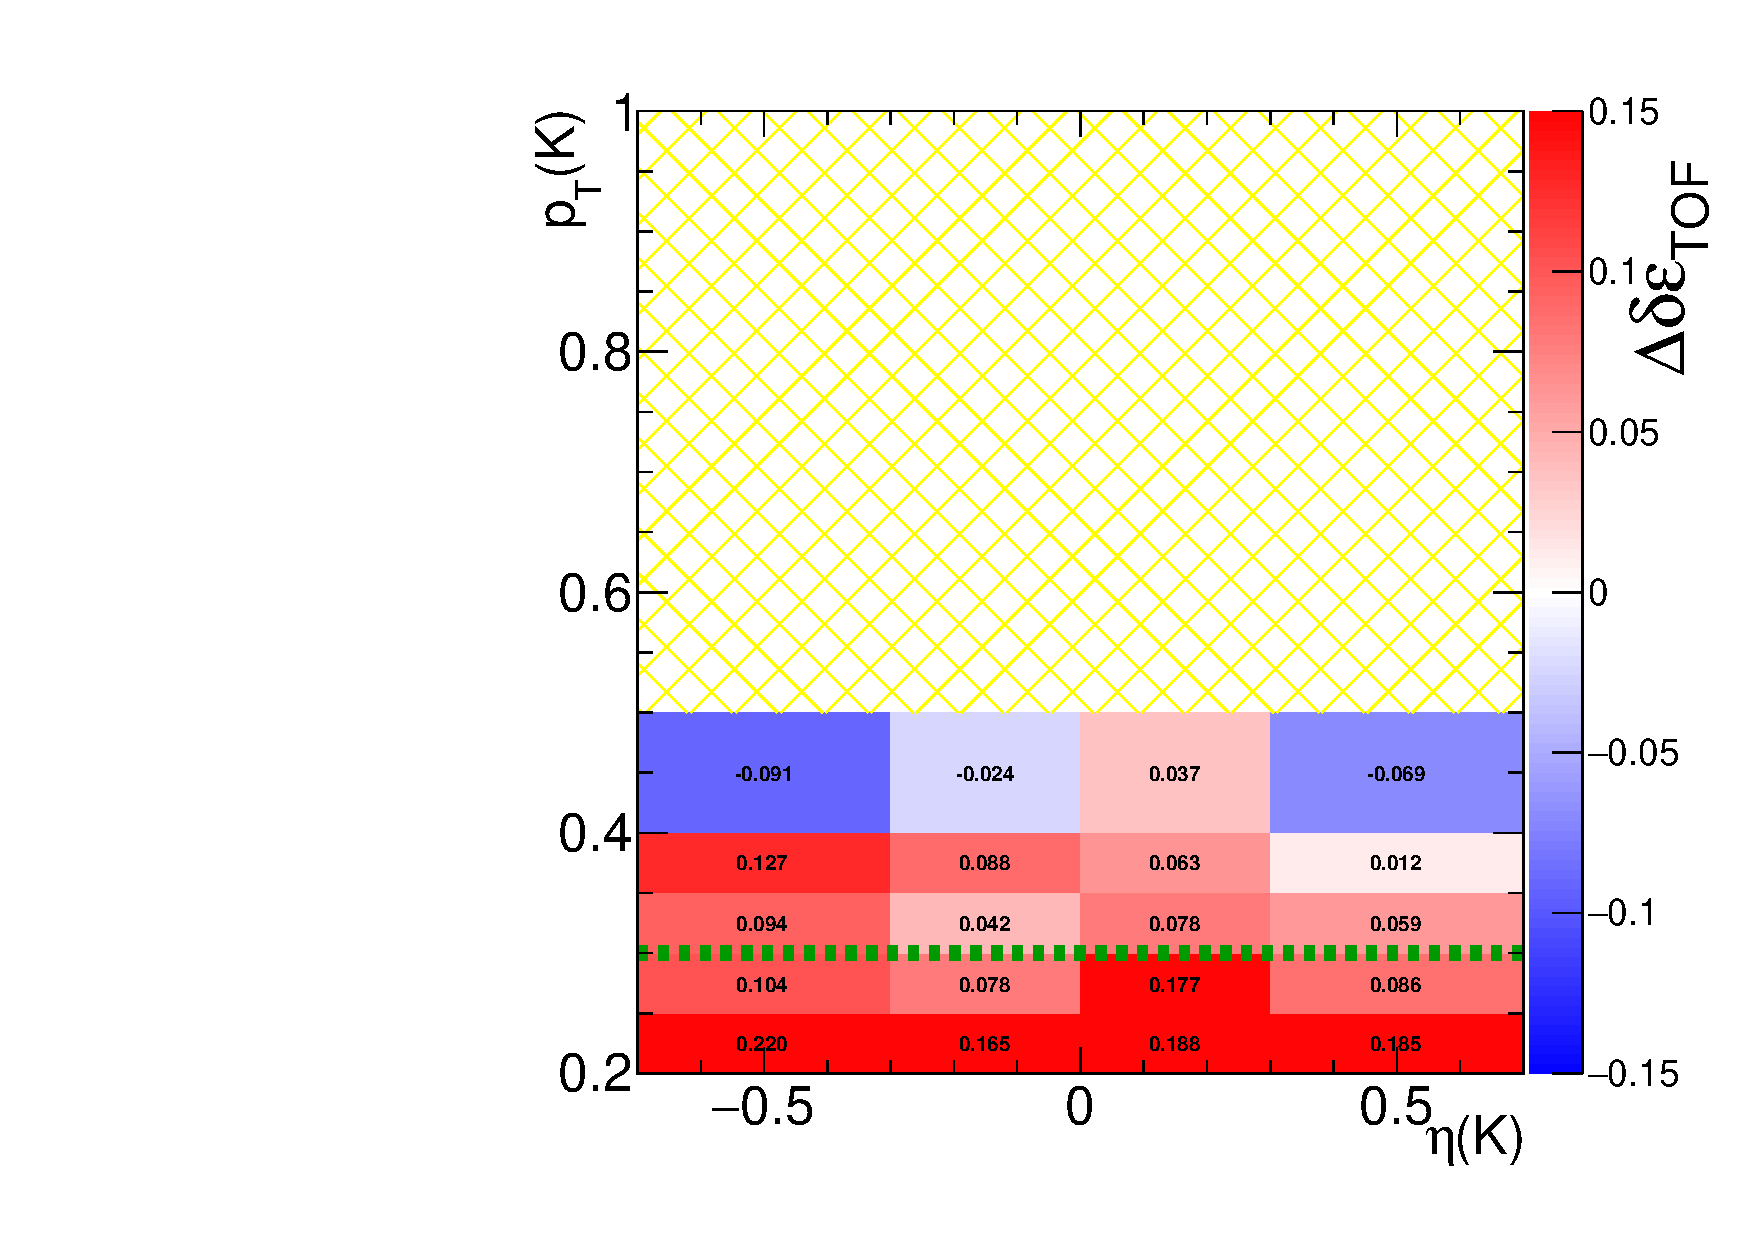
\includegraphics[width=\linewidth]{graphics/systematicsEfficiency/TofSyst/tofEffDifference_Delta_kaon.pdf}\vspace{-12pt}}}
  \end{subfigure}
} 
\quad
\parbox{0.31\textwidth}{
  \centering
  \begin{subfigure}[b]{\linewidth}{
                \subcaptionbox{\label{fig:tofEffDifference_Delta_proton}}{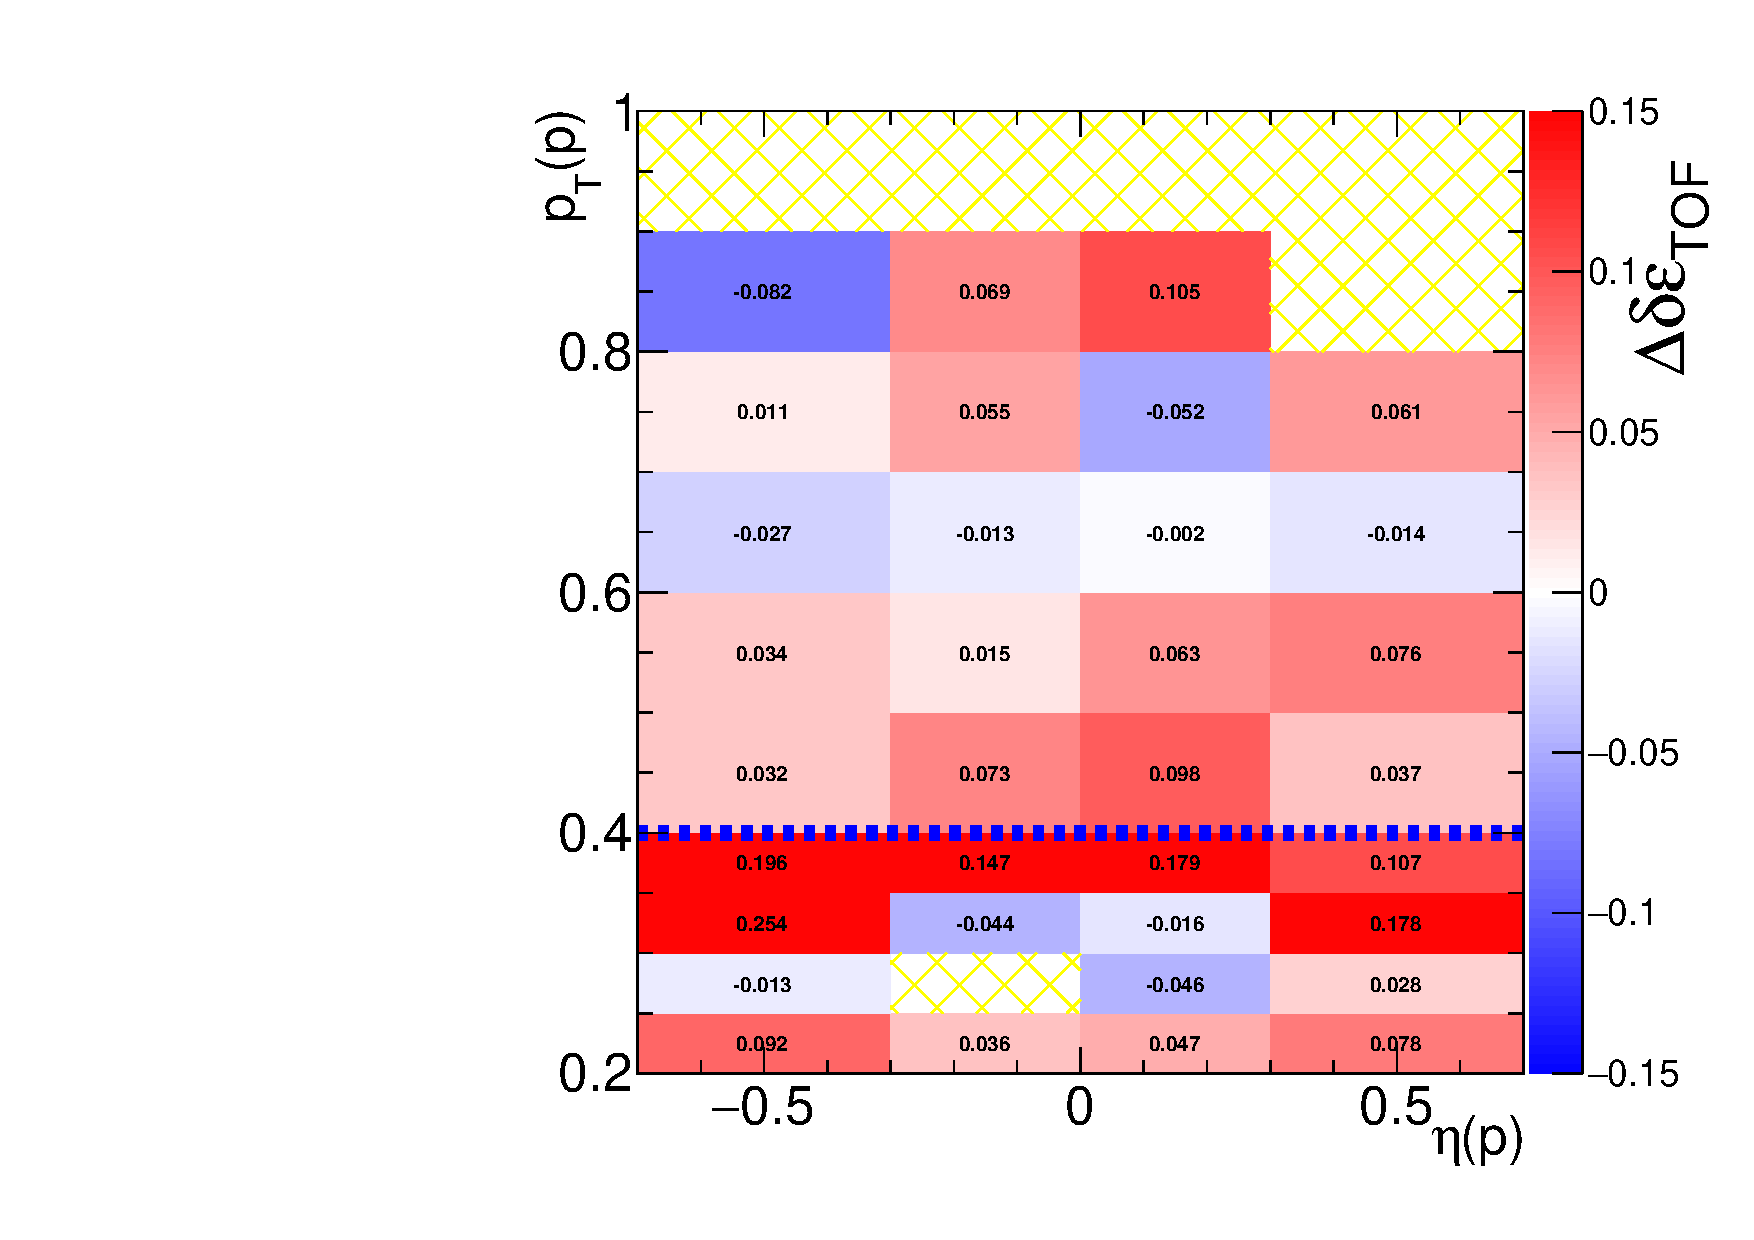
\includegraphics[width=\linewidth]{graphics/systematicsEfficiency/TofSyst/tofEffDifference_Delta_proton.pdf}\vspace{-12pt}}}
  \end{subfigure}
}
\caption[Difference between the TOF eff. correction estimated with the HFT-tagged tracks and with tag\&probe method.]%
    {Difference between the TOF eff. correction estimated with the HFT-tagged tracks for pions (\ref{fig:tofEffDifference_Delta_pion}), kaons (\ref{fig:tofEffDifference_Delta_kaon}) and protons (\ref{fig:tofEffDifference_Delta_proton}), and the correton from tag\&probe method on CEP $\pi^{+}\pi^{-}$ events. Figure \ref{fig:tofEffDifference_Delta_pion} is the difference between \ref{fig:tofEffDifference_pion} and \ref{fig:TPcorrectionTofEff2D}, Figure \ref{fig:tofEffDifference_Delta_kaon} is the difference between \ref{fig:tofEffDifference_kaon} and \ref{fig:TPcorrectionTofEff2D}, and Figure \ref{fig:tofEffDifference_Delta_proton} is the difference between \ref{fig:tofEffDifference_proton} and \ref{fig:TPcorrectionTofEff2D}. Yellow hatched area mark bins which were empty in histograms for HFT-tagged tracks (thus difference is incalculable). Dashed horizontal lines represent minimum track $p_{T}$ thresholds used in our analyses: $0.3$~GeV for kaons (green) and $0.4$~GeV for protons (blue).}\label{fig:tofEffDifference_Delta}% 
\end{figure}
%---------------------------

The effective systematic uncertainty calculated as an average uncertainty weigthed with the MC events is shown in Fig.~\ref{fig:tofSystError}. From the Figure one reads that the uncertainty for a pion, kaon and proton track is of the order of 1\%, 3\% and 2\%, respectively.

%---------------------------
\begin{figure}[h]
\centering
\parbox{0.4725\textwidth}{
  \centering
  \begin{subfigure}[b]{\linewidth}
                \subcaptionbox{\label{fig:tofSystError_pT}}{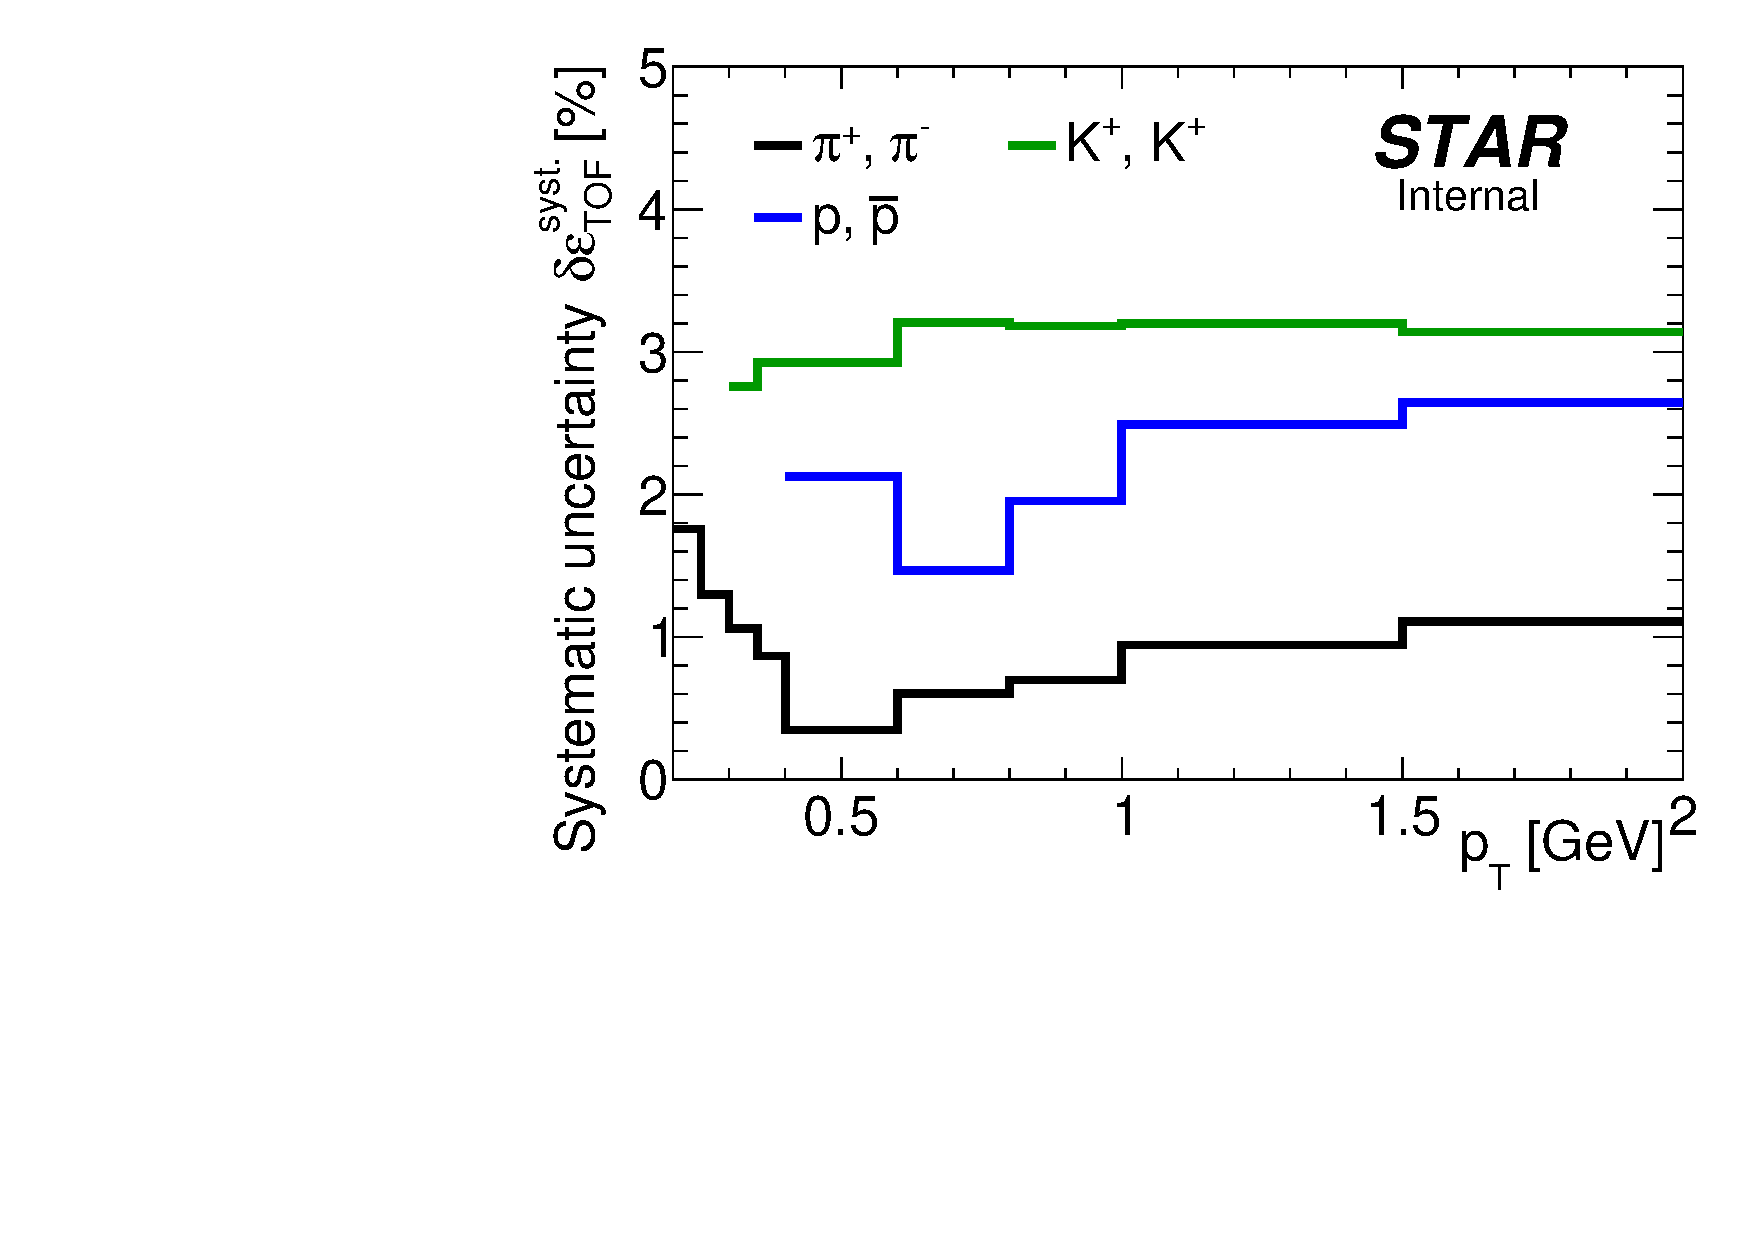
\includegraphics[width=\linewidth]{graphics/systematicsEfficiency/TofSyst/TofSystError_pT.pdf}\vspace{-10pt}}\vspace{-6pt}
  \end{subfigure}
}%
\quad\quad%
\parbox{0.4725\textwidth}{
  \centering
  \begin{subfigure}[b]{\linewidth}
                \subcaptionbox{\label{fig:tofSystError_eta}}{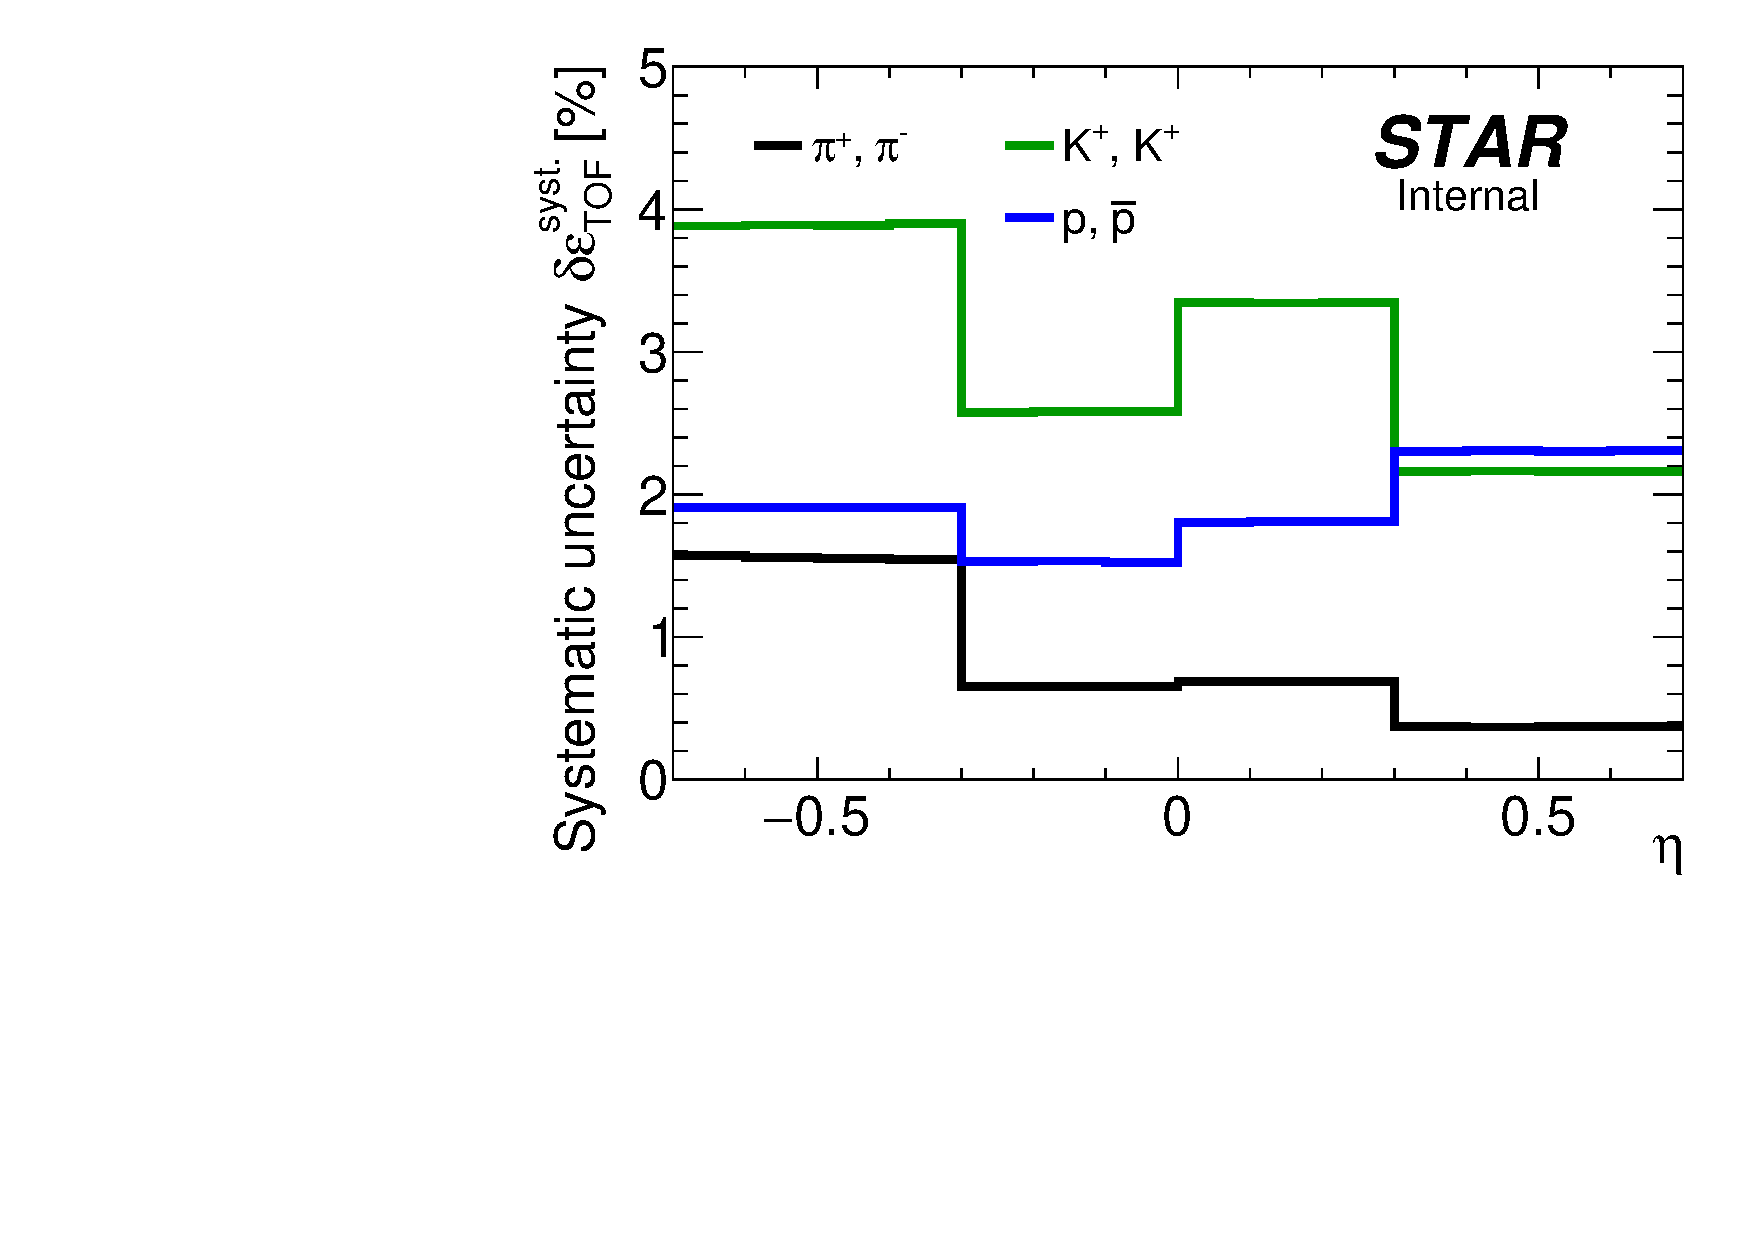
\includegraphics[width=\linewidth]{graphics/systematicsEfficiency/TofSyst/TofSystError_eta.pdf}\vspace{-10pt}}\vspace{-6pt}
  \end{subfigure}
}%
\caption[Systematic uncertainty of the TOF efficiency related to the TOF simulation accuracy.]% 
    {Effective systematic uncertainty of the TOF efficiency related to the simulation accuracy, drawn as a function of the track $p_{T}$ (\ref{fig:tofSystError_pT}) and track $\eta$ (\ref{fig:tofSystError_eta}). The $p_{T}$-dependence was calculated for tracks within $|\eta|<0.7$, while $\eta$-dependence was calculated for tracks with $p_{T}$ greater than the threshold established for given particle type (see Sec.~\ref{sec:TpcQualityCuts}).}\label{fig:tofSystError}%
\end{figure}
%---------------------------



\section{Roman Pot track reconstruction efficiency}\label{sec:rpTrackRecoEffSystematics}

\subsection{Track reconstruction efficiency (absolute reconstruction efficiency)}\label{subsec:rpTrackRecoEffSyst}

Nominally the RP track reconstruction efficiency is calculated with the zero-bias-embedded MC events as a probability that forward scattered proton is transported from the IP to the RP stations and produces hits in SSDs that are reconstructed as a track point(s) that form a track which passes selection cuts. The systematic uncertainty of this efficiency, which reflects the accuracy of the simulation (modeling of the dead material, signal digitization etc.), has been estimated using elastic scattering events. The same analysis scheme was used for the data and for embedded elastic scattering MC events. The difference between efficiency estimates extracted from the data and simulation was established as a measure of the systematic uncertainty of the nominal RP track reconstruction efficiency.

Obviously, in our physics analyses we study processes other than elastic proton-proton scattering, nevertheless the difference between the result obtained with data and simulated elastic scattering MC events are a good measure of the systematic uncertainty also for other processes. We choose elastic scattering for this study as it is the cleanest process involving forward protons - backgrounds can be suppressed relatively easy with the collinearity constraint. In addition to this, parameters of the proton track (its momentum, position in the detector) can be reconstructed even in case of lack of signal in one or both detectors in a branch. An additional argument to use elastic scattering is that in CEP of low central masses ($\lesssim3$~GeV) forward protons have $\xi\approx0$, rarely exceeding $0.05$ in studied rapidity range of the central state.% For SD and CD analysis an addional 

%---------------------------
\begin{figure}[h]%\vspace{-34pt}
	\centering
	\parbox{0.65\textwidth}{%
		\centering%
		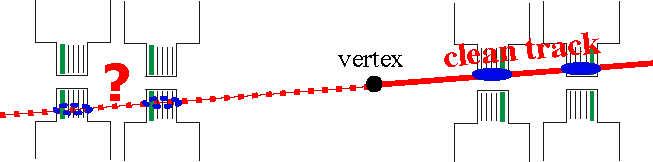
\includegraphics[width=\linewidth]{graphics/systematicsEfficiency/RpSyst/effCalculationScheme.pdf}%
	} 
	\quad
	\parbox{0.31\textwidth}{ 
		\centering
		%\begin{minipage}[t][0.64\linewidth][t]{\linewidth}%\vspace{73pt} 
			\caption[Draft of the method of estimation of the RP track reconstruction efficiency for systematic uncertainty determination.]%
			{Sketch of the Roman Pot system with drafted method of estimation of the RP track reconstruction efficiency using elastic scattering events.}\label{fig:sketchRpTrackEffSyst}% 
		%\end{minipage}
	}
	
\end{figure}
%---------------------------

An idea of presented analysis was to select elastic proton-proton scattering events by requiring the elastic trigger (signal in PMTs in two opposite RP branches) and clean RP track of $\xi$ consistent with 0 within $3.5\sigma_{\xi}$ on one side of the IP, and counting how often there is reconstructed and successfully selected collinear RP track in the opposite branch with trigger signal. The method is illustrated in Fig.~\ref{fig:sketchRpTrackEffSyst}. Detailed description of the algorithm is provided below:
\begin{enumerate}
\item RP\_ET triggers were used. Elastic proton-proton scattering MC events (generated with $B=14.3~\text{GeV}^{-2}$ as it was measured in independent analysis, see Ref.~\cite{ElasticNote}) simulated in Geant4 and embedded into zero-bias data were subjected to the same trigger conditions (signal in trigger counters in opposite RP branches was required). The zero-bias data used in embedding was taken from the same runs for which RP\_ET triggers were analyzed. Also number of simulated events for each run was proportional to number of elastic scattering events in given run.\vspace{-4pt}
\item Since RP\_ET triggers can be fired not only by elastic interactions but also, for instance, by central diffraction events, minimum bias events with forward remnants of protons, overlap of single diffraction events with beam halo protons, etc., a list of vetoes was exerted to suppress non-elastic interaction/pile-up:\vspace*{-7pt}
\begin{multicols}{3}
	\begin{itemize}
		\item TOF L0 mulitplicity = 0
		\item n. of TPC-TOF tracks = 0
		\item n. of recon. TOF hits = 0
		\item empty ZDC
		\item empty VPD
		\item empty BBC (small, large)
		\item false state of RP\_IT trigger bit (trigger signal only in RP branches forming an elastic trigger bit RP\_ET)
	\end{itemize}
\end{multicols}\vspace{-10pt}
As shown in Fig.~\ref{fig:rpSystXi_EU}, the mentioned types of background events that fire RP\_ET trigger are vastly suppressed with the above vetoes.\vspace{-4pt}
\item From the difference between average time of the trigger signal in west and east RPs the $z$-position of the vertex was reconstructed and required to satisfy condition $|z_{\text{vtx}}|<80$~cm, which is the same as the range of $z_{\text{vtx}}$ accepted in our physics analyses.\vspace{-4pt}
\item One side (a 'tagging' side, or a reference side) was checked if a clean set of track points was reconstructed in a branch with trigger signal. By clean set of track points we understand either 1 and 0, 0 and 1, or 1 and 1 reconstructed track point in the $1^{\text{st}}$ and $2^{\text{nd}}$ RP in given branch, respectively. If yes, from this(ese) track point(s) a RP track was formed, reconstructed with the $z$-position of the vertex assumed to be as it was reconstructed in \#3. Fractional momentum loss of this track was required to be $|\xi|<0.01$ (Fig.\ref{fig:rpSystXi_EU}).\vspace{-4pt}
\item Checked if in the 'probed' branch (that has a trigger signal, opposite to the reference branch) there is RP track which passes the track selection used in CEP analysis, and there is exactly 1 such track (as in CEP analysis):\vspace*{-4pt}% (criteria \textbf{C4} in Ref.~\cite{AnalysisNoteRafal}).
\begin{itemize}
  \itemm RP track contains only track-points with at least 3 (out of maximum 4) planes used in reconstrucion,
  \itemm Local angles are consistent with the forward proton track originating from the IP:\vspace{-5pt}
  \[-2~\text{mrad}<\theta_{x}^{\text{RP}}-x^{\text{RP}}/|z^{\text{RP}}|<4~\text{mrad},~~~~~-2~\text{mrad}<\theta_{y}^{\text{RP}}-y^{\text{RP}}/|z^{\text{RP}}|<2~\text{mrad}\]
\end{itemize}\vspace{-4pt}
If the above was satisfied, the collinearity was calculated between the track reconstructed in the branch under study and the reference track (Fig.~\ref{fig:rpSystCollinearity}). If the collinearity was within 3.5 standard deviations ($\sigma_{\Delta\theta_{x}} \approx \sigma_{\Delta\theta_{y}} \approx 180~\mu\text{rad}$) the elastic track was claimed reconstructed.
\end{enumerate}

%---------------------------
\begin{figure}[t!]%\vspace{-34pt} 
	\centering
	\parbox{0.4725\textwidth}{%
		\centering%
		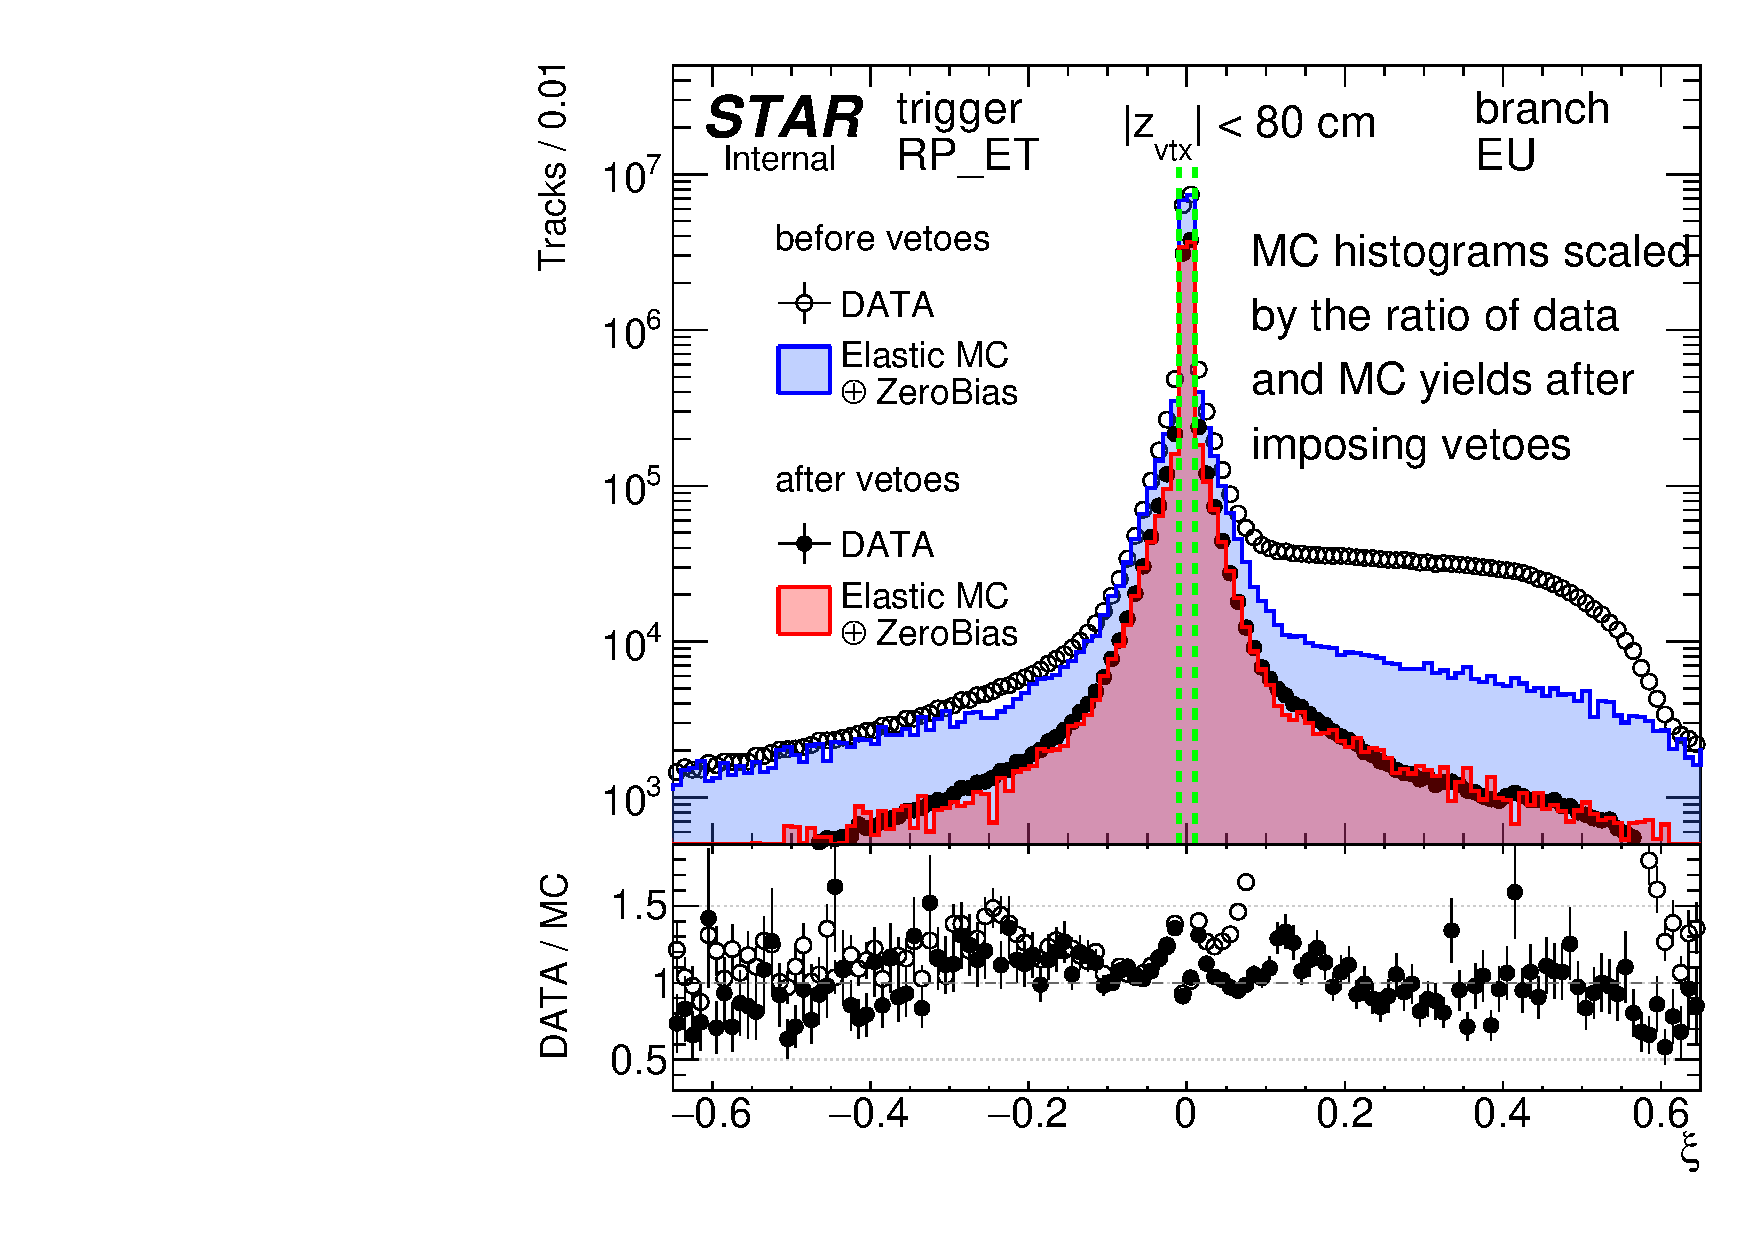
\includegraphics[width=\linewidth,page=1]{graphics/systematicsEfficiency/RpSyst/xiPerBranch.pdf}%
	} 
	\quad
	\parbox{0.4725\textwidth}{ 
		\centering
		%\begin{minipage}[t][0.64\linewidth][t]{\linewidth}%\vspace{73pt} 
			\caption[Fractional momentum loss $\xi$ of clean proton tracks before and after implying vetoes in the data and MC (branch EU).]%
			{Fractional momentum loss $\xi$ of clean proton tracks in branch EU before and after implying vetoes. Data are represented by opened and filled circles, while elastic MC embedded into zero-bias data is drawn as filled histograms. MC histograms are scaled by the ratio of data and MC yields after imposing vetoes in other STAR detector subsystems. Lower pad shows the ratio of corresponding distributions in the data and MC. Before vetoes are applied a significant contribution of non-elastic forward protons in the data sample is clearly visible (excees over MC for $\xi>0.01$). Satisfactory agreement between the data and MC is found after imposing vetoes, which indicates successfull purification of data sample. Dashed green vertical lines show the $\xi$ range of tracks accepted for the RP track (and also track point) efficiency studies, $|\xi|<0.01$. Similar plot for the remaining branches can be found in Appendix~\ref{appendix:rpTrackRecoEffSyst}.}\label{fig:rpSystXi_EU}%  
		%\end{minipage}
	}
	
\end{figure}
%---------------------------


%---------------------------
\begin{figure}[b!]
\centering
\parbox{0.4725\textwidth}{
  \centering
  \begin{subfigure}[b]{\linewidth}
                \subcaptionbox{\label{fig:rpSystCollinearity_x}}{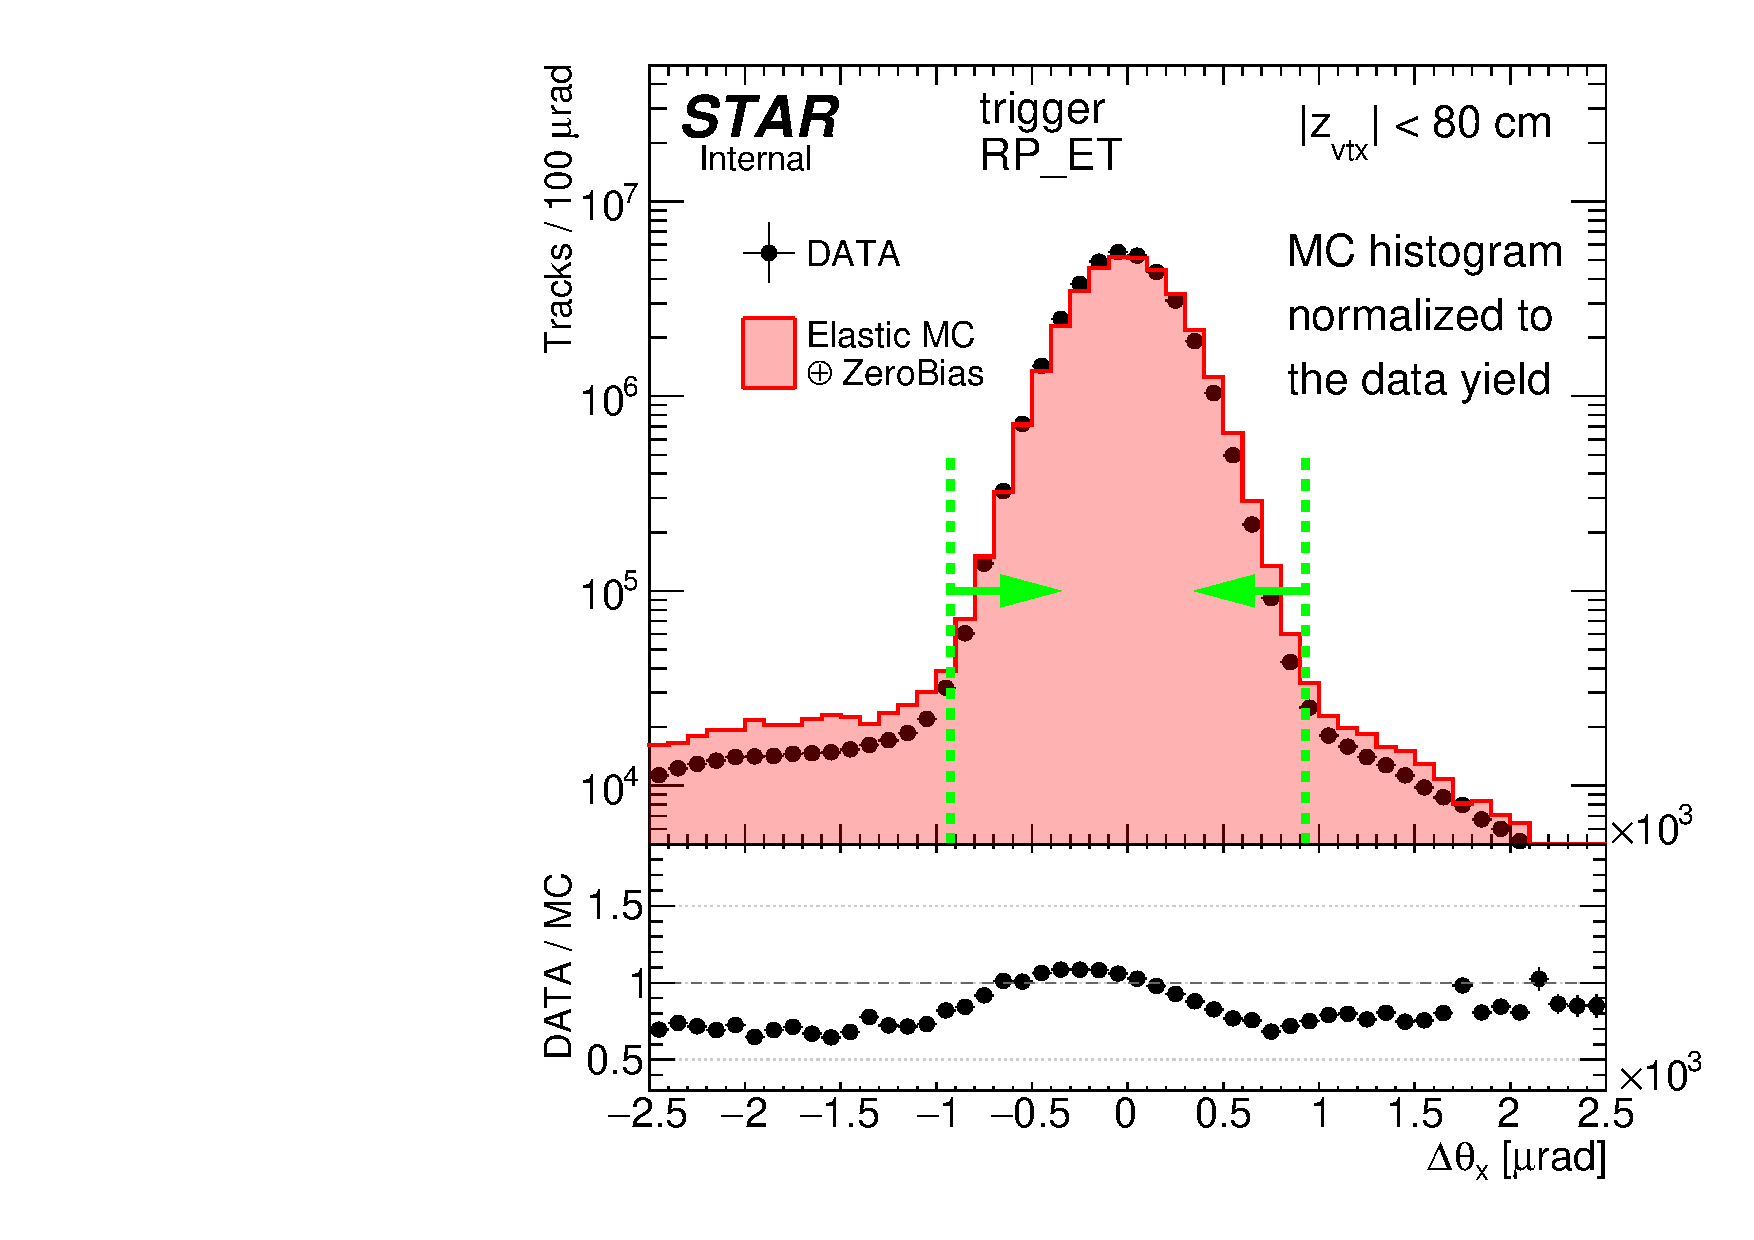
\includegraphics[width=\linewidth,page=1]{graphics/systematicsEfficiency/RpSyst/collinearity.pdf}\vspace{-7pt}}
  \end{subfigure}
}%
\quad\quad%
\parbox{0.4725\textwidth}{
  \centering
  \begin{subfigure}[b]{\linewidth}
                \subcaptionbox{\label{fig:rpSystCollinearity_y}}{\includegraphics[width=\linewidth,page=2]{graphics/systematicsEfficiency/RpSyst/collinearity.pdf}\vspace{-7pt}}
  \end{subfigure}
}%
\caption[Collinearity of a reference track and track reconstructed in studied branch.]% 
    {Collinearity of a reference track (the clean track which is required to have $|\xi|<0.01$) and track reconstructed in branch for which reconstruction efficiency is studied, separately in $xz$-plane (Fig.~\ref{fig:rpSystCollinearity_x}) and $yz$-plane (Fig.~\ref{fig:rpSystCollinearity_y}). An elastic track is claimed as reconstructed if the collinearity of two tracks does not exceed 3.5 standard deviations, as marked with dashed green vertical lines and arrows.}\label{fig:rpSystCollinearity}%
\end{figure}
%---------------------------

\begin{enumerate}\setcounter{enumi}{5}
\item The RP track reconstruction efficiency $\varepsilon$ was defined as a probability that in the studied branch exactly 1 RP track was reconstructed and selected, and found collinear with the reference track within 3.5 standard deviations (as required in \#5). It was calculated as a ratio of the number of events with reconstructed track in a probed branch and clean track in tagging branch, to all number of events with clean track in tagging branch.\vspace{-4pt}
\item Steps \#4-\#6 were repeated for the other side.
\end{enumerate}


The efficiencies obtained with the described method were calculated as a function of the expected transverse momentum components of the proton in the branch under study. These components were assumed to be equal to the $(p_{x},p_{y})$ of the track in the tagging branch taken with the "-" sign to reflect the fact that elastically scattered protons have opposite momentum, $(p_{x}^{\text{E}},p_{y}^{\text{E}},p_{z}^{\text{E}}) = (-p_{x}^{\text{W}},-p_{y}^{\text{W}},-p_{z}^{\text{W}})$ (in the center-of-mass reference frame, which here is identical with the laboratory frame). The sample result for a single branch is presented in Fig.~\ref{fig:totalRpRecoEff_EU}. The remaining results were placed in Appendix~\ref{appendix:rpTrackRecoEffSyst}.


%---------------------------
\begin{figure}[h]\vspace{-10pt}
	\centering
	\parbox{0.54\textwidth}{
		\centering
		\begin{subfigure}[b]{\linewidth}{\vspace{10pt}
				\subcaptionbox{\label{fig:totalRpRecoEff2D_EU}}{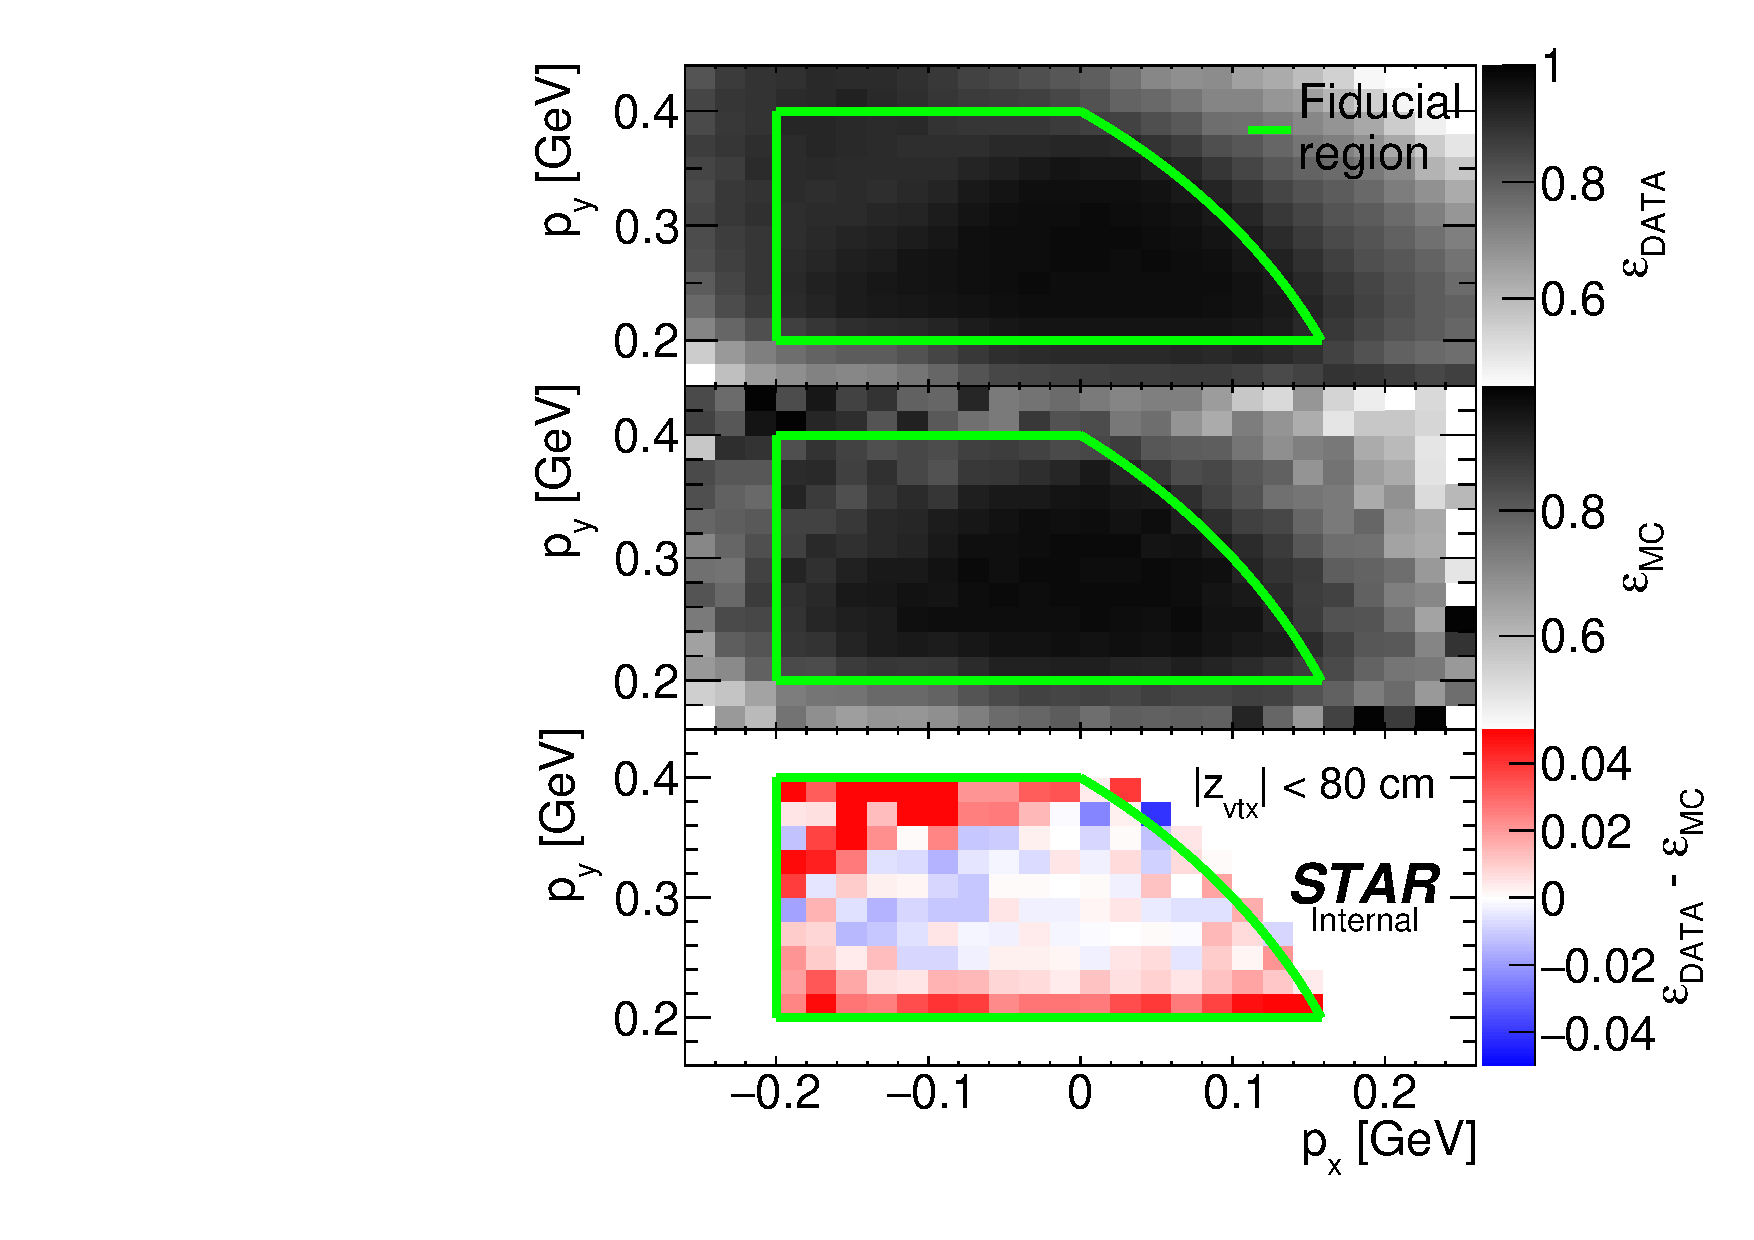
\includegraphics[width=\linewidth,page=1]{graphics/systematicsEfficiency/RpSyst/totalRpRecoEff2D.pdf}\vspace{-12pt}}}
		\end{subfigure}
  \begin{minipage}[t][0.64\linewidth][t]{\linewidth}\vspace{5pt}
	\caption[Coparison of estimated RP track reconstruction efficiency in 2D and 1D (branch EU).]%
	{Sample comparison of RP track reconstruction efficiency (branch EU) estimated with the method described in the text as a function of $(p_{x},p_{y})$ of proton track (\ref{fig:totalRpRecoEff2D_EU}) and comparison of 1-dimensional projections of efficiencies in a fiducial region marked with green envelope: $p_{x}$ (\ref{fig:totalRpRecoEff1D_EU_px}) and $p_{y}$ (\ref{fig:totalRpRecoEff1D_EU_py}). Dashed orange line marks the border of the fiducial region part where the correction to RP track reconstruction efficiency is required. Lower pad in each subfigure shows the difference between efficiency extracted from the data and elastic scattering MC embedded into zero-bias data. Hatched orange area marks bins without any entries (efficiency incalculable). The difference between efficiencies in Fig.~'\ref{fig:totalRpRecoEff2D_EU} was calculated only for entries in the fiducial region. Similar plots for the remaining branches can be found in Appendix~\ref{appendix:rpTrackRecoEffSyst}.%
	}\label{fig:totalRpRecoEff_EU}
	\end{minipage}
	\vspace{14pt}%
	}
	\quad
	\parbox{0.43\textwidth}{\vspace{-15pt}
		\centering
		\begin{subfigure}[b]{\linewidth}{
				\subcaptionbox{\label{fig:totalRpRecoEff1D_EU_px}}{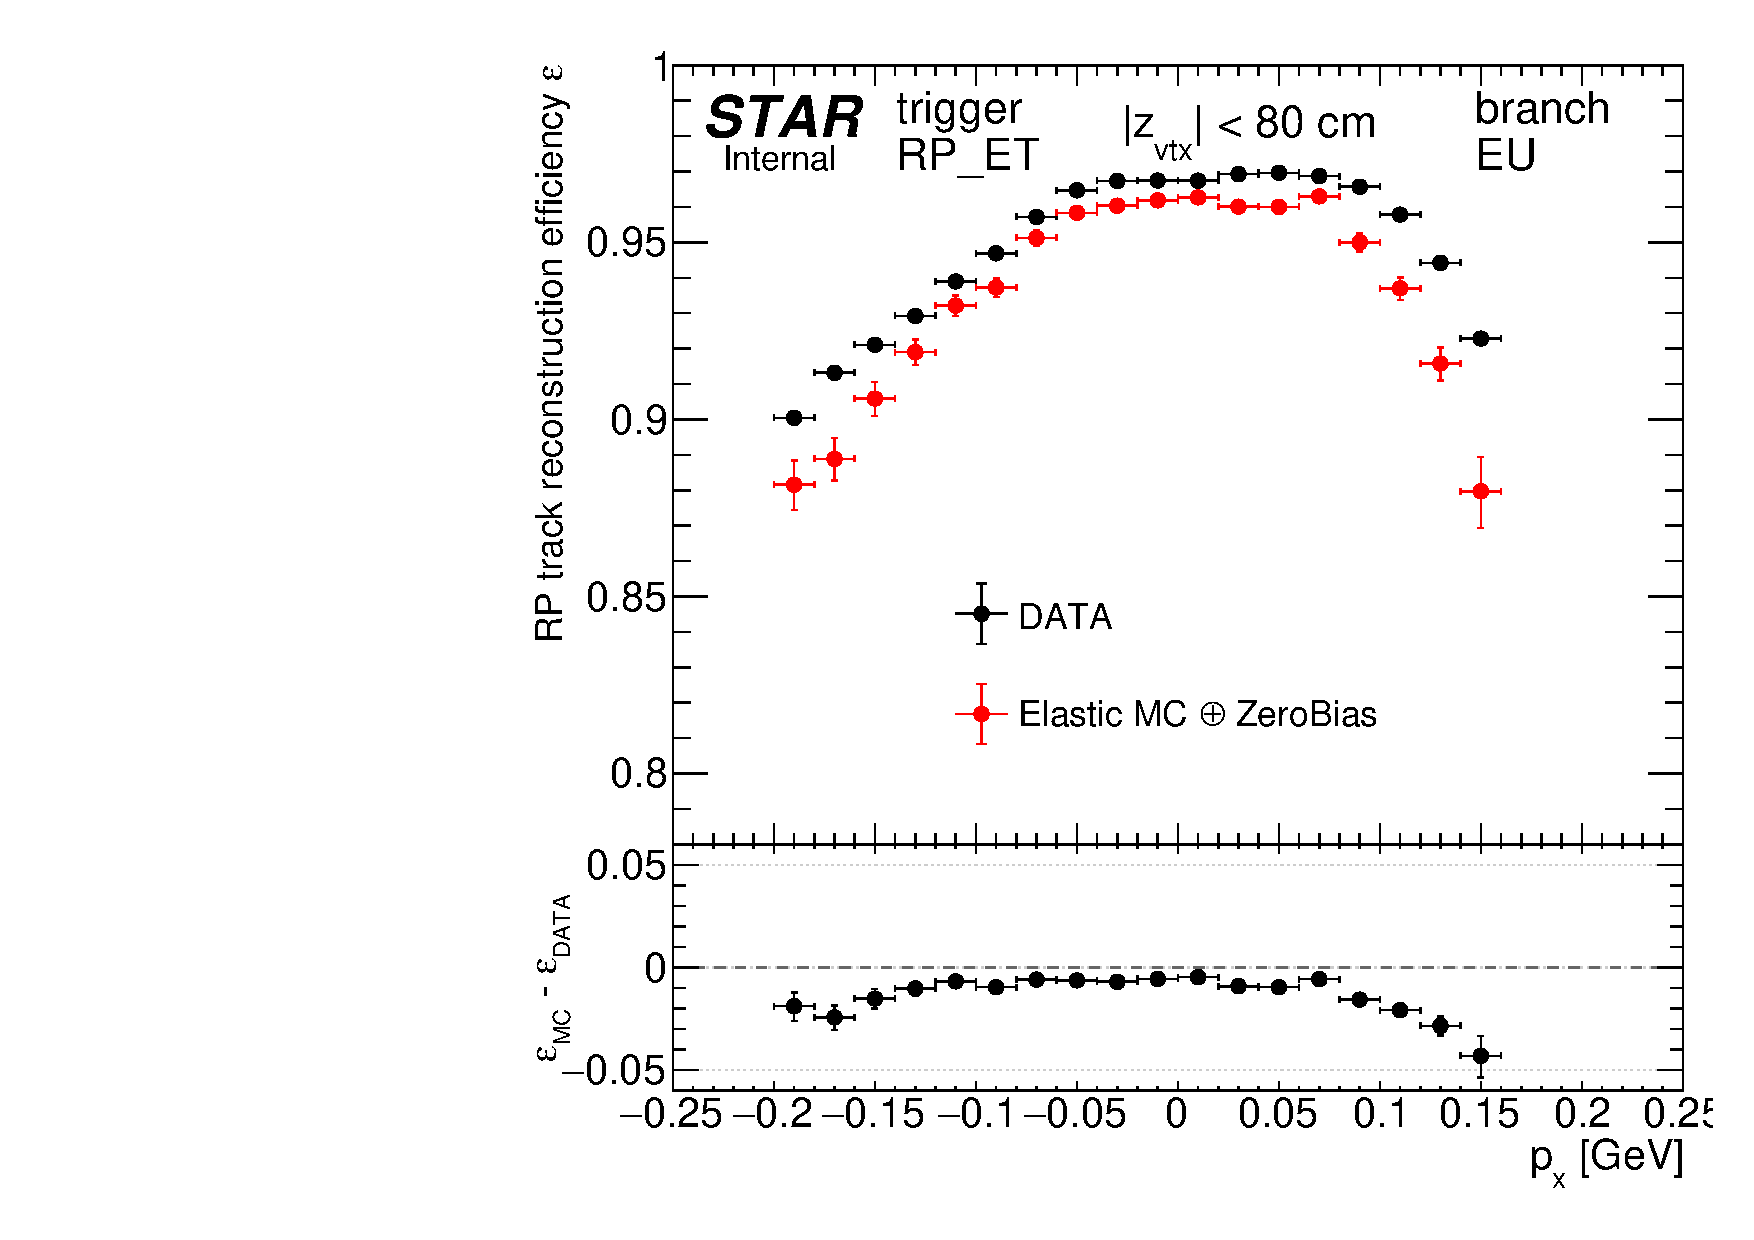
\includegraphics[width=\linewidth,page=1]{graphics/systematicsEfficiency/RpSyst/dataTotalEff_1D.pdf}\vspace{-12pt}}}
		\end{subfigure}
		\begin{subfigure}[b]{\linewidth}{
				\subcaptionbox{\label{fig:totalRpRecoEff1D_EU_py}}{\includegraphics[width=\linewidth,page=2]{graphics/systematicsEfficiency/RpSyst/dataTotalEff_1D.pdf}\vspace{-12pt}}}
		\end{subfigure}
	}
\end{figure}
%---------------------------


From the figures one can read that the difference between the RP track reconstruction efficiency estimated from the data and from embedded MC do not differ by more than $\sim5\%$. In the central part of the fiducial region used in CEP analysis, defined by Ineqs.~\eqref{eq:fiducialPxPy} as
\begin{equation}\label{eq:fiducialPxPy}
 0.2<|p_{y}|<0.4,~~~-0.2<p_{x},~~~(p_{x}+0.3)^{2}+p_{y}^{2}<0.5^{2}~~~(\text{all in GeV}),
\end{equation}
where sensitivity to the edge effects (uncertainty on aperture positions), to dead material effects and to inaccuracies in simulated angular beam divergence is suppressed, the difference is not larger than $\sim1\%$. Such number was taken as the uncertainty on the track reconstruction efficiency related to the signal digitization and embedding and the track reconstruction algorithm. The largest difference between the data and simulation is observed in the corner of the fiducial region satisfying Ineq.~\eqref{eq:fiducialPxPyCorner}
\begin{equation}\label{eq:fiducialPxPyCorner}
(p_{x}-0.2)^{2}+p_{y}^{2}>0.46^{2}~~~(\text{all in GeV}),
\end{equation}
where the RF shield is present between the $1^{\text{st}}$ and $2^{\text{nd}}$ RP station, and possibly also the front part of the DX-D0 chamber is present. This may indicate that the thickness/density of these elements is not accurately modeled (too thick/dense pieces of material implemented in the simulation). %
% More significant differences are generally observed close to the edges of the fiducial region rather than its center. This could be an influence of the angular beam divergence which was assumed constant in the simulation, while in the data it changes over time (grows with the RHIC store lifetime). 
We decided to introduce correction to the RP track reconstruction efficiency in the corner of the fiducial region (Ineq.~\ref{eq:fiducialPxPyCorner}), equal to the difference between data and MC track reconstruction efficiency estimates presented in Fig.\ref{fig:totalRpRecoEff2D_EU} (and corresponding plots for other branches). We assign a conservative systematic uncertainty to the efficiency in this corner region equal to the absolute value of the efficiency correction. We may conduct an independent analysis of this corner region in order to have better, more realistic estimate od the systematic uncertainty.


For the remaining part of the fiducial $(p_{x},p_{y})$ region we also assign a systematic uncertainty of the RP track reconstruction efficiency equal to the absolute value of the difference between data and MC track reconstruction efficiency estimates shown in Fig.~\ref{fig:totalRpRecoEff2D_EU} and in Appendix~\ref{appendix:rpTrackRecoEffSyst}. These differences should also cover uncertainties related to the angular beam divergence effects and error on positions of limiting apertures.















\subsection{Track point reconstruction efficiency (relative reconstruction efficiency)}\label{subsec:rpTrackPointRecoEffSyst}

A single track point reconstruction efficiency can be studied in a way similar to the track reconstruction efficiency. In contrast to the latter, to estimate track point reconstruction efficiency one can reconstruct elastic scattering event independently from the studied detector, which provides even higher purity of the sample in comparison to the track reconstruction efficiency.

The comparison between track point reconstruction efficiency in the data and simulation provides better insight to discrepancies in detector geometry and amount of material than comparison of track reconstruction efficiency, as in this case the effect of angular beam divergence is reduced by using proton track observables reconstructed on the side of studied RP detector. Relative RP efficiency is mostly sensitive to material in between the RPs in the same branch, as the presence of elastic track reconstructed in the studied branch assures that proton survived transport from the IP to RP stations. This study gives us also information about performance of the track-point reconstrucion algorithm itself.

Unfortunately, information about the track point reconstruction efficiency is limited - there is no access to some part of the fiducial region, approximately described by inequality $p_{x}\lessapprox-0.08$~GeV. This is caused by the fact that RPs in the $1^{\text{st}}$ and the $2^{\text{nd}}$ station do not fully overlap - they are shifted with respect to each other, with the most significant offset in $x$ direction ($\approx2$~cm) due to restrictions imposed on DX-D0 chamber at the design level, mainly to acommodate space for ZDC detectors place close behind the $2^{\text{nd}}$ RP stations.

\begin{figure}[h]%\vspace{-34pt}
	\centering
	\parbox{0.65\textwidth}{%
		\centering%
		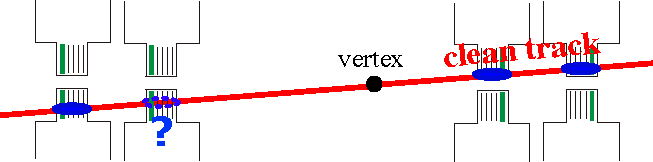
\includegraphics[width=\linewidth]{graphics/systematicsEfficiency/RpSyst/effCalculationScheme_2.pdf}%
	} 
	\quad
	\parbox{0.31\textwidth}{ 
		\centering
		%\begin{minipage}[t][0.64\linewidth][t]{\linewidth}%\vspace{73pt}
			\caption[Draft of the method of estimation of the RP track point reconstruction efficiency for systematic uncertainty determination.]%
			{Sketch of the Roman Pot system with drafted method of estimation of the RP track point reconstruction efficiency using elastic scattering events.}\label{fig:sketchRpTrackPointEffSyst}% 
		%\end{minipage}
	}
	
\end{figure}
%---------------------------

In this analysis elastic proton-proton scattering events were selected by requiring the elastic trigger (signal in PMTs in two opposite RP branches) and clean RP track of $|\xi|<0.01$ on one side of the IP, and clean track point with trigger signal in at least one RP (a reference RP) in the opposite branch. A track was formed from this clean track point and the two tracks were required collinear within 3.5 standard deviations. In the other RP detector in a studied branch a trigger was required. The probability to have exactly 1 track point in the studied RP with position consistent with that extrapolated from the reference RP was referred to as the track point reconstruction efficiency. The method is illustrated in Fig.~\ref{fig:sketchRpTrackPointEffSyst}. Detailed description of the algorithm is provided below, excluding steps \#1-\#4 which are the same as in Sec.~\ref{subsec:rpTrackRecoEffSyst}:


\begin{enumerate}\setcounter{enumi}{4}%
\item Selected one RP station with a trigger signal in the studied branch (opposite to the tagging branch). We call it a reference detector. A clean track point in that RP was required. By clean track point we understand exactly 1 track point, in addition reconstructed with at least 3 (out of 4) silicon planes. A track was formed from the track point in the reference detector. Collinearity was calculated between the tagging track and the track reconstructed from the clean track point in studied branch (Fig.~\ref{fig:rpSystCollinearity}). If the collinearity was satisfied within 3.5 standard deviations the reference elastic track was claimed reconstructed.\vspace{-4pt}
\item The trigger signal was required in the detector under study (the other detector in the same branch as a reference detector). The RP track point reconstruction efficiency $\varepsilon$ was defined as a probability that in the studied RP, among unlimited number of reconstructed track points exactly 1 track point had reconstructed $(x,y)$ position consistent with the position extrapolated from the reference detector $(x_{\text{extr}},y_{\text{extr}})$ within $1.2$~mm (Fig.~\ref{fig:rpSystPositionDifference}). It was calculated as a ratio of the number of selected elastic scattering events with a trigger signal in a studied detector, and exactly 1 track point of reconstructed position matching the expected, to all number of selected elastic scattering events with a trigger signal in the studied detector.\vspace{-4pt}
\item Steps \#5-\#6 were repeated for the other detector in studied branch.\vspace{-4pt}
\item Steps \#5-\#7 were repeated for the other side.
\end{enumerate}

%---------------------------
\begin{figure}[h]
\centering
\parbox{0.4725\textwidth}{
  \centering
  \begin{subfigure}[b]{\linewidth}
                \subcaptionbox{\label{fig:rpSystPositionDifference_x}}{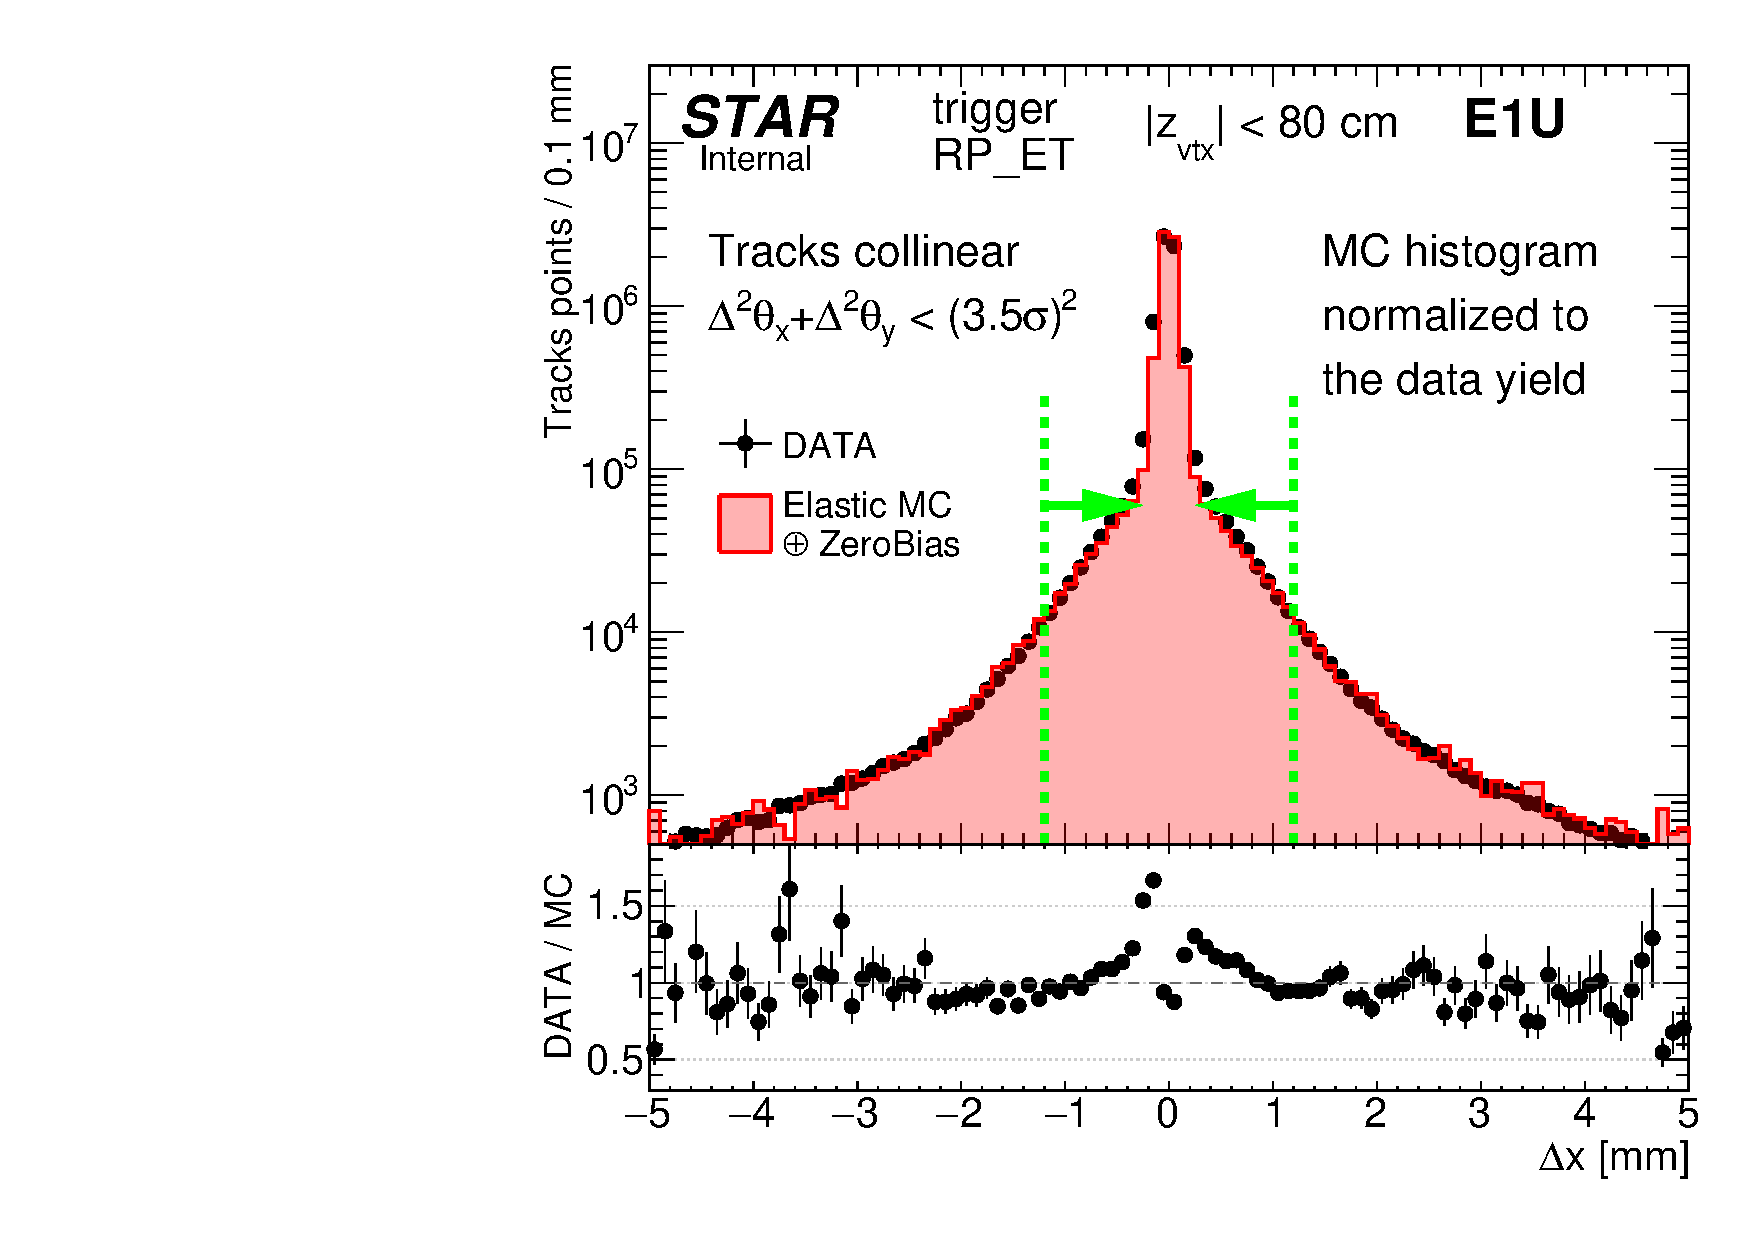
\includegraphics[width=\linewidth,page=1]{graphics/systematicsEfficiency/RpSyst/positionDifference.pdf}\vspace{-7pt}}
  \end{subfigure}
}%
\quad\quad%
\parbox{0.4725\textwidth}{
  \centering
  \begin{subfigure}[b]{\linewidth}
                \subcaptionbox{\label{fig:rpSystPositionDifference_y}}{\includegraphics[width=\linewidth,page=2]{graphics/systematicsEfficiency/RpSyst/positionDifference.pdf}\vspace{-7pt}}
  \end{subfigure}
}%
\caption[Difference between measured and extrapolated position of track point in E1U.]%
    {Difference between position of a track point (with clusters in 3 out 4 silicon planes) reconstructed in E1U (if E1U has a trigger signal) and expected track point position extrapolated from a reference track point reconstructed in E2U, for elastic scattering events with the collinearity of the track in the opposite branch and track reconstructed from a reference track point better than 3.5 standard deviations. A track point is claimed as reconstructed if the position difference is not larger than 1.2~mm, as marked with dashed green vertical lines and arrows.}\label{fig:rpSystPositionDifference}%
\end{figure}
%---------------------------

The estimates of track point reconstruction efficiency obtained with the described method are shown in Figs.~\ref{fig:relativeRpRecoEff_E1U} (E1U), \ref{fig:relativeRpRecoEff_E2U} (E2U) and Appendix~\ref{appendix:rpTrackRecoEffSyst} (for the remaining). They are presented 2-dimensionally: in $(p_{x},p_{y})$ (Figs.~\ref{fig:relativeRpRecoEff2D_E1U_pxpy}, \ref{fig:relativeRpRecoEff2D_E2U_pxpy}) and $(x,y)$ (Figs.~\ref{fig:relativeRpRecoEff2D_E1U_xy}, \ref{fig:relativeRpRecoEff2D_E2U_xy}), as well as 1-dimensionally: in $x$ (Figs.~\ref{fig:relativeRpRecoEff1D_E1U_x}, \ref{fig:relativeRpRecoEff1D_E2U_x}) and $y$ (Figs.~\ref{fig:relativeRpRecoEff1D_E1U_y}, \ref{fig:relativeRpRecoEff1D_E2U_y}).


In the area of detector accessible in this study an excellent agreement ($<0.5\%$ difference) between the efficiency estimates from data and MC is found in the region of no material on the proton path from IP to the RPs. This reflects correct simulation of the silicon signal digitization, cluster reconstruction and matching, track point reconstruction and embedding. The differences between data and MC are more significant in the region of aperture shadows, e.g. DX shadow visible the best in Fig.~\ref{fig:relativeRpRecoEff1D_E1U_x} at $x \gtrapprox 20$~mm (possibly too much simulated material), or DX-D0 chamber entry/RF shield shadow visible in Fig.~\ref{fig:relativeRpRecoEff1D_E1U_y} at $y \gtrapprox 60$~mm (probably also too much simulated material).

%---------------------------
\begin{figure}[h]%\vspace{-34pt}  
	\centering
	\parbox{0.4725\textwidth}{
		\centering
		\begin{subfigure}[b]{\linewidth}{%\vspace{10pt}
				\subcaptionbox{\label{fig:relativeRpRecoEff2D_E1U_pxpy}}{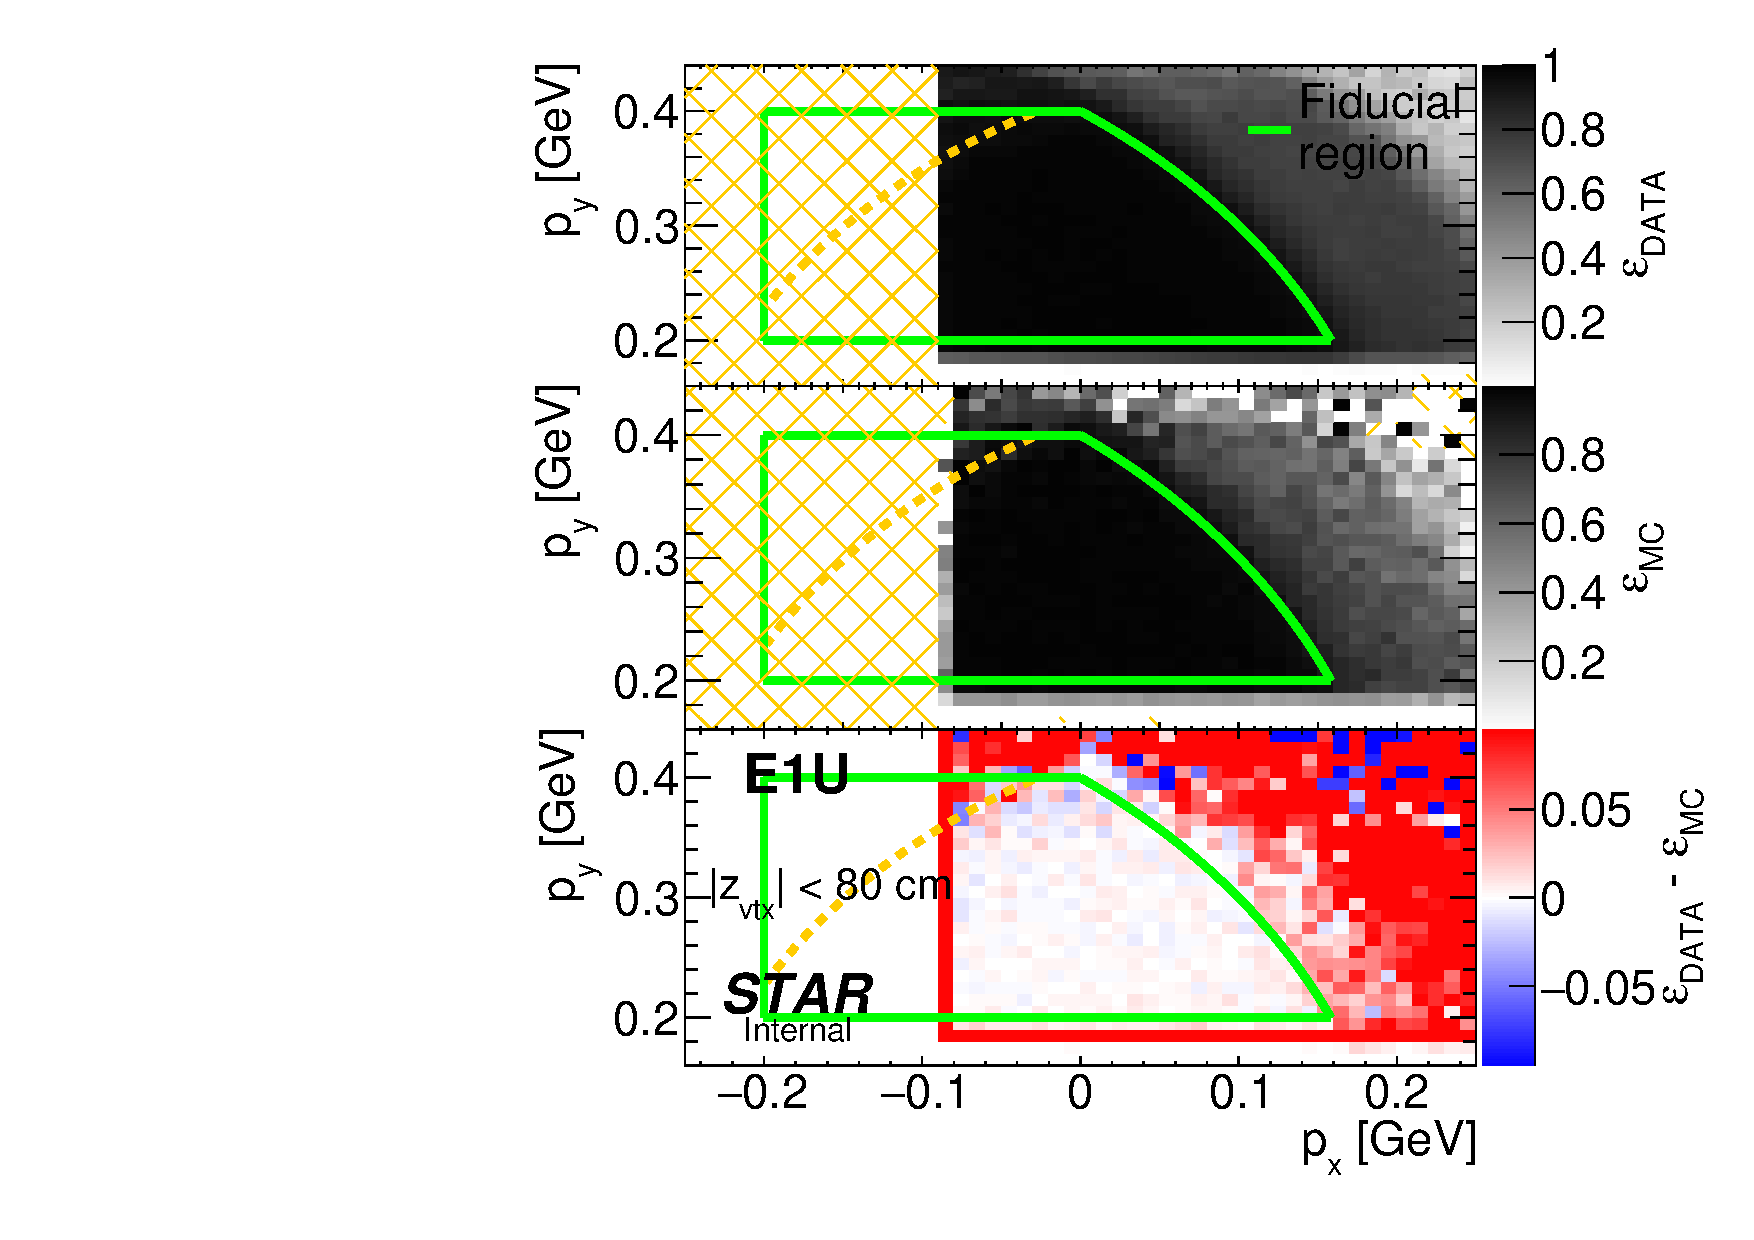
\includegraphics[width=\linewidth,page=1]{graphics/systematicsEfficiency/RpSyst/relativeRpRecoEff2D_pxpy.pdf}\vspace{-12pt}}}
		\end{subfigure}
		\begin{subfigure}[b]{\linewidth}{\addtocounter{subfigure}{1}{
				\subcaptionbox{\label{fig:relativeRpRecoEff1D_E1U_x}}{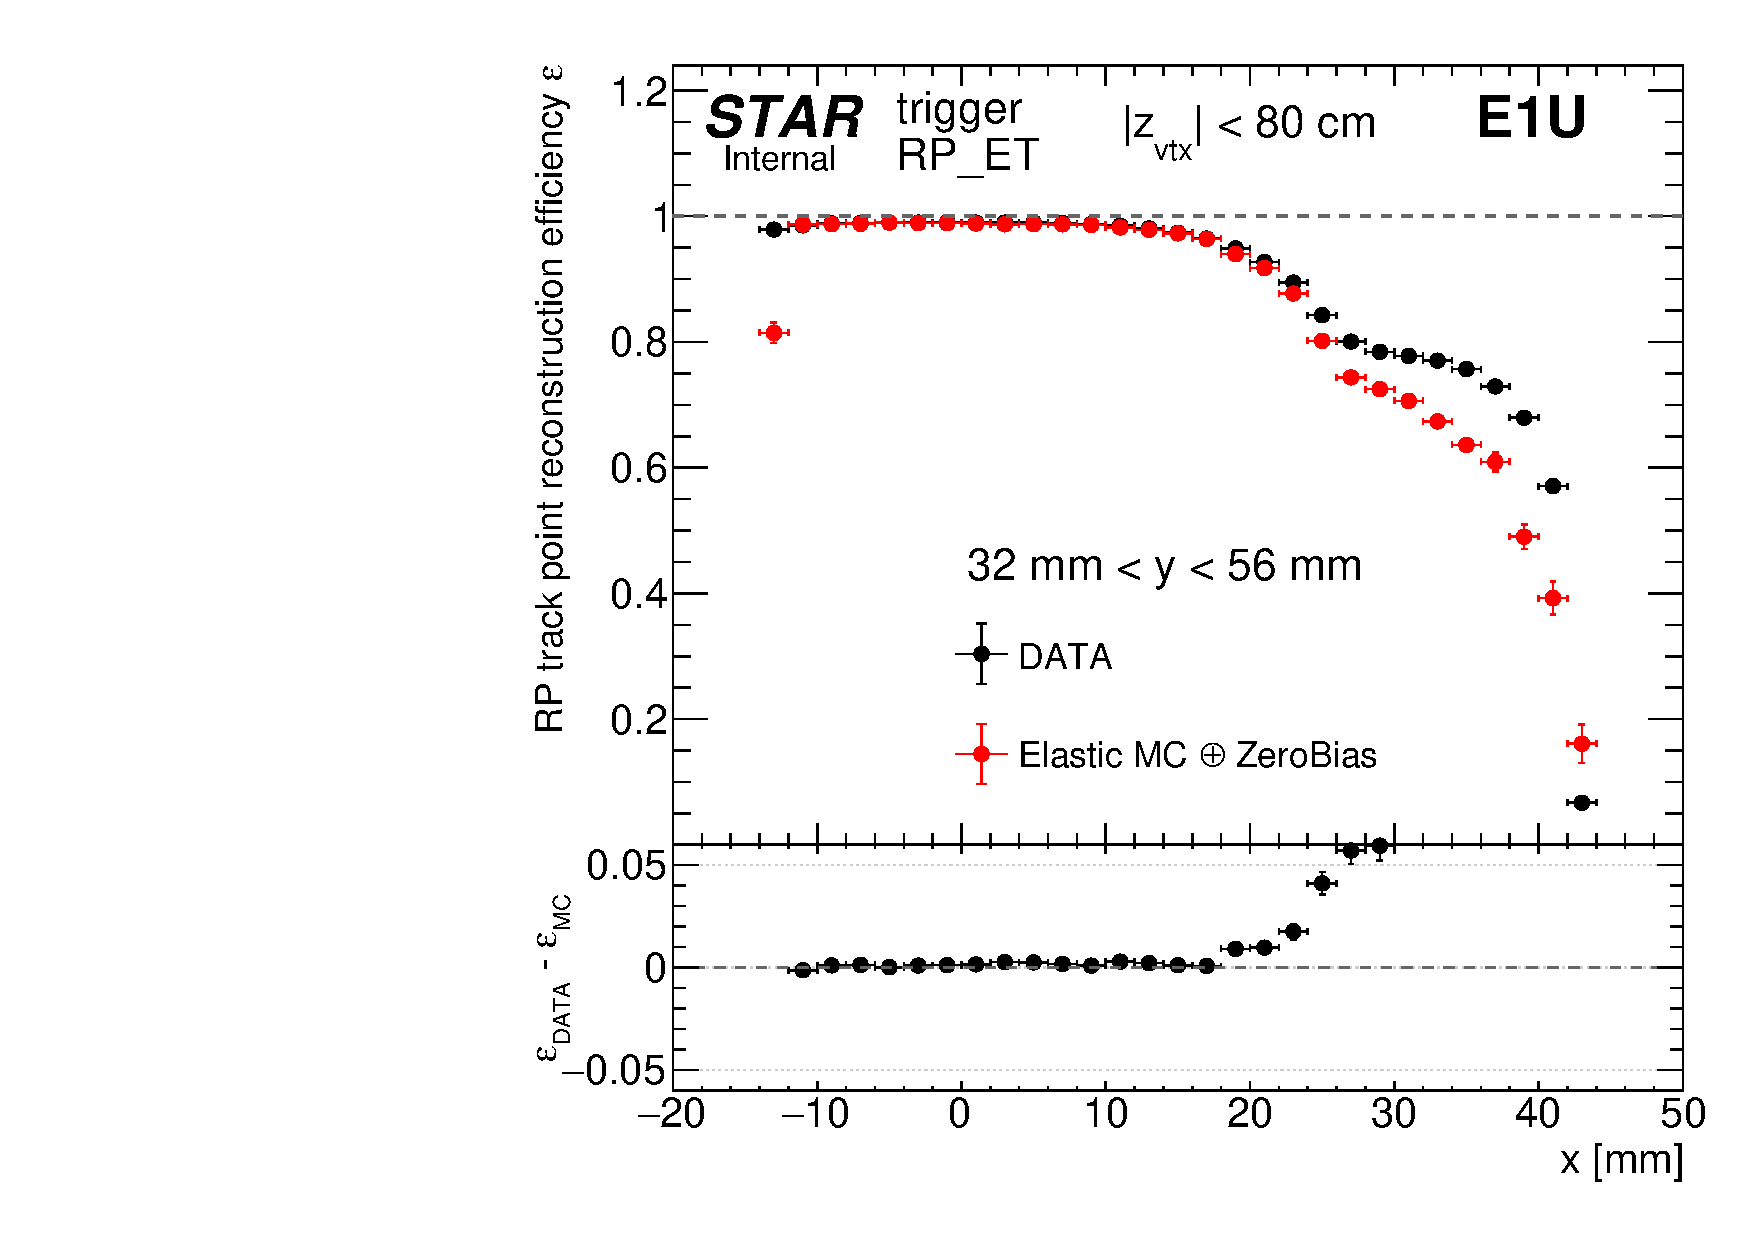
\includegraphics[width=\linewidth,page=1]{graphics/systematicsEfficiency/RpSyst/dataRelativeEff_1D.pdf}\vspace{-12pt}}}}
		\end{subfigure}
	}
	\quad
	\parbox{0.4725\textwidth}{
		\centering
		\begin{subfigure}[b]{\linewidth}{\addtocounter{subfigure}{-2}{%\vspace{10pt} 
				\subcaptionbox{\label{fig:relativeRpRecoEff2D_E1U_xy}}{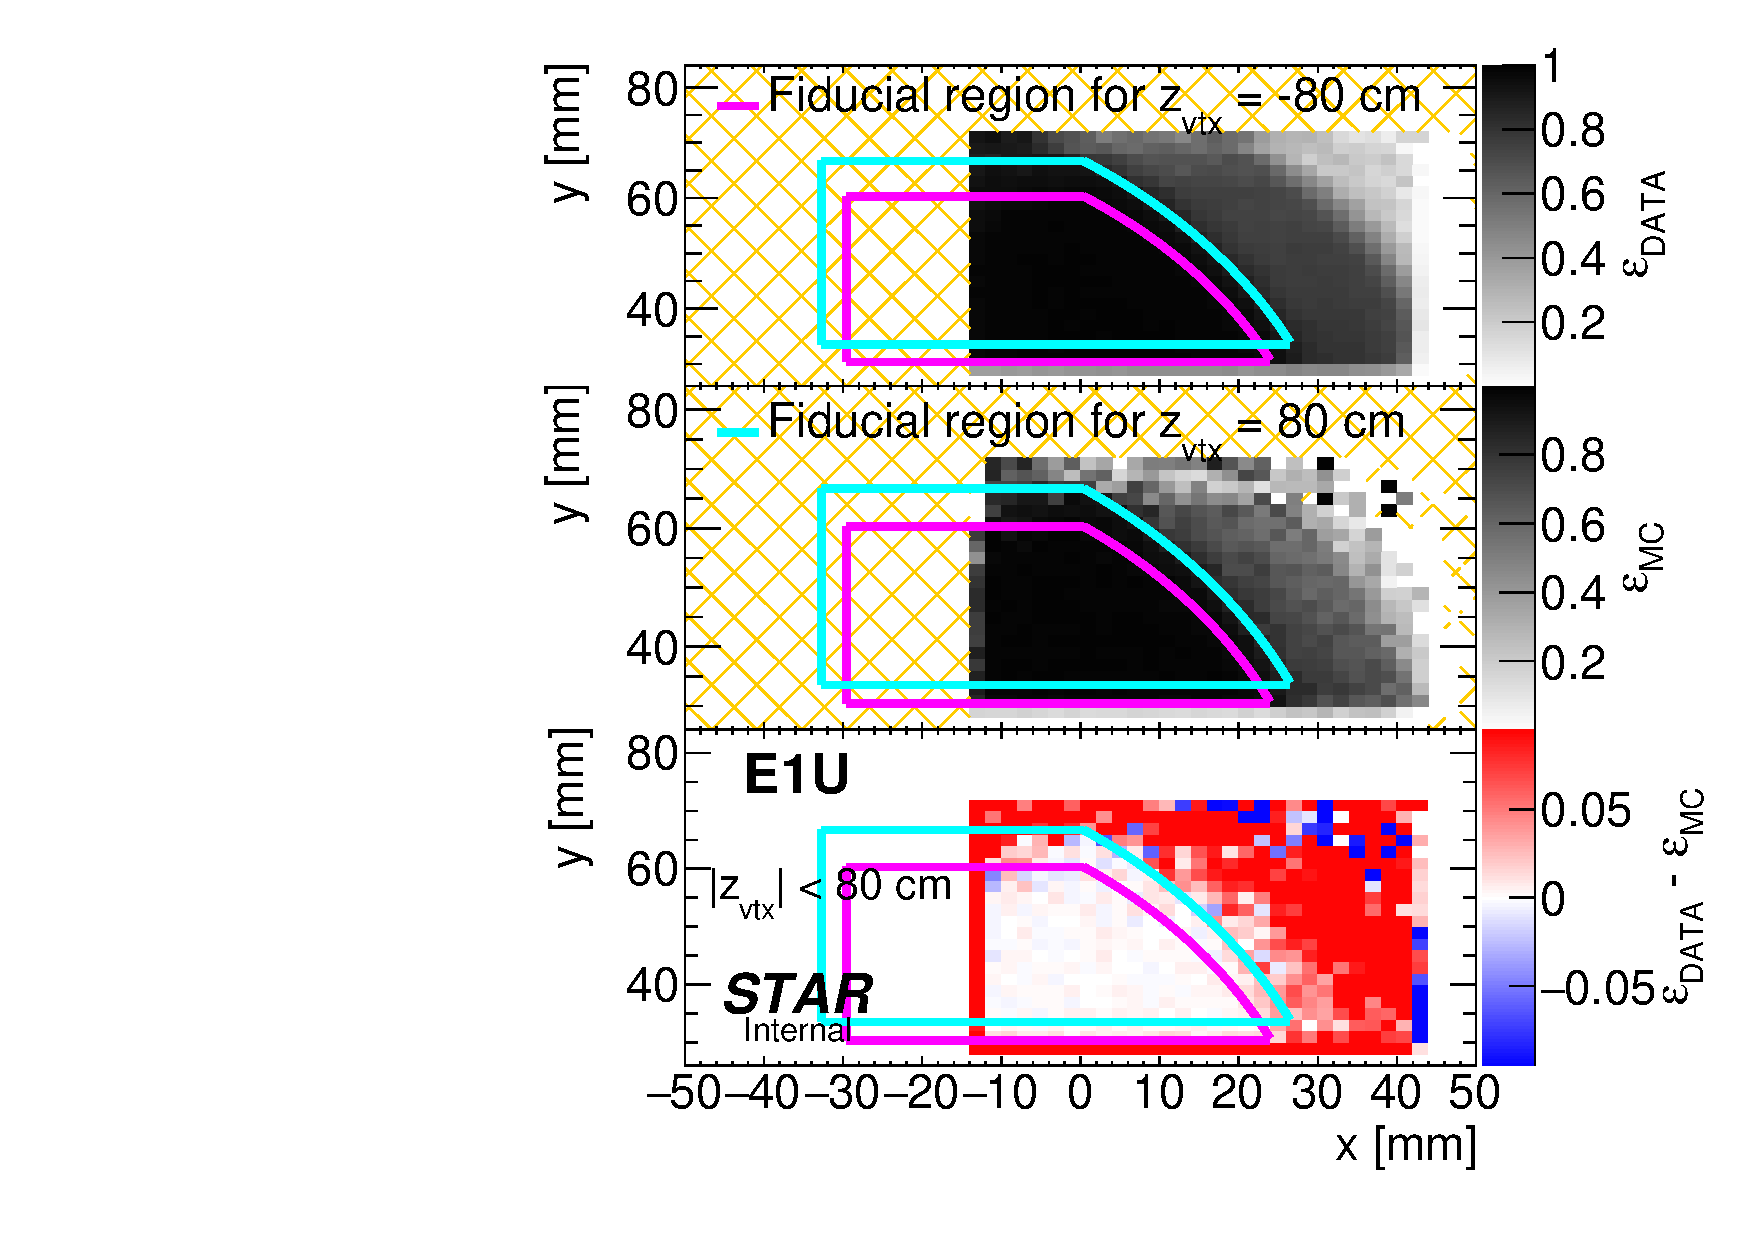
\includegraphics[width=\linewidth,page=1]{graphics/systematicsEfficiency/RpSyst/relativeRpRecoEff2D.pdf}\vspace{-12pt}}}}
		\end{subfigure}
		\begin{subfigure}[b]{\linewidth}{\addtocounter{subfigure}{1}{
				\subcaptionbox{\label{fig:relativeRpRecoEff1D_E1U_y}}{\includegraphics[width=\linewidth,page=2]{graphics/systematicsEfficiency/RpSyst/dataRelativeEff_1D.pdf}\vspace{-12pt}}}}
		\end{subfigure}
	}
	\caption[Coparison of estimated RP track point reconstruction efficiency in 2D and 1D (detector E1U).]%
	{Sample comparison of RP track point reconstruction efficiency (detector E1U) estimated with the method described in the text as a function of $(p_{x},p_{y})$ of proton track (\ref{fig:relativeRpRecoEff2D_E1U_pxpy}), $(x,y)$ position extrapolated from the reference RP (E2U) to the studied RP (\ref{fig:relativeRpRecoEff2D_E1U_xy}), and comparison of 1-dimensional projections of efficiencies in selected ranges of hit position (given in the plot): $x$ (\ref{fig:relativeRpRecoEff1D_E1U_x}) and $y$ (\ref{fig:relativeRpRecoEff1D_E1U_y}). Lower pad in each subfigure shows the difference between efficiency extracted from the data and elastic scattering MC embedded into zero-bias data. Hatched orange area marks bins without any entries (efficiency incalculable). The fiducial region in $(x,y)$ plot is represented by two envelopes which correspond to the extreme accepted values of $z_{vtx}$. Similar plots for the remaining detectors can be found in Appendix~\ref{appendix:rpTrackRecoEffSyst}.% 
	}\label{fig:relativeRpRecoEff_E1U}
\end{figure}
%---------------------------



%---------------------------
\begin{figure}[h]%\vspace{-34pt}  
	\centering
	\parbox{0.4725\textwidth}{
		\centering
		\begin{subfigure}[b]{\linewidth}{%\vspace{10pt}
				\subcaptionbox{\label{fig:relativeRpRecoEff2D_E2U_pxpy}}{\includegraphics[width=\linewidth,page=2]{graphics/systematicsEfficiency/RpSyst/relativeRpRecoEff2D_pxpy.pdf}\vspace{-12pt}}}
		\end{subfigure}
		\begin{subfigure}[b]{\linewidth}{\addtocounter{subfigure}{1}{
				\subcaptionbox{\label{fig:relativeRpRecoEff1D_E2U_x}}{\includegraphics[width=\linewidth,page=3]{graphics/systematicsEfficiency/RpSyst/dataRelativeEff_1D.pdf}\vspace{-12pt}}}}
		\end{subfigure}
	}
	\quad
	\parbox{0.4725\textwidth}{
		\centering
		\begin{subfigure}[b]{\linewidth}{\addtocounter{subfigure}{-2}{%\vspace{10pt} 
				\subcaptionbox{\label{fig:relativeRpRecoEff2D_E2U_xy}}{\includegraphics[width=\linewidth,page=2]{graphics/systematicsEfficiency/RpSyst/relativeRpRecoEff2D.pdf}\vspace{-12pt}}}}
		\end{subfigure}
		\begin{subfigure}[b]{\linewidth}{\addtocounter{subfigure}{1}{
				\subcaptionbox{\label{fig:relativeRpRecoEff1D_E2U_y}}{\includegraphics[width=\linewidth,page=4]{graphics/systematicsEfficiency/RpSyst/dataRelativeEff_1D.pdf}\vspace{-12pt}}}}
		\end{subfigure}
	}
	\caption[Coparison of estimated RP track point reconstruction efficiency in 2D and 1D (detector E2U).]%
	{Sample comparison of RP track point reconstruction efficiency (detector E2U) estimated with the method described in the text as a function of $(p_{x},p_{y})$ of proton track (\ref{fig:relativeRpRecoEff2D_E2U_pxpy}), $(x,y)$ position extrapolated from the reference RP (E1U) to the studied RP (\ref{fig:relativeRpRecoEff2D_E2U_xy}), and comparison of 1-dimensional projections of efficiencies in selected ranges of hit position (given in the plot): $x$ (\ref{fig:relativeRpRecoEff1D_E2U_x}) and $y$ (\ref{fig:relativeRpRecoEff1D_E2U_y}). Lower pad in each subfigure shows the difference between efficiency extracted from the data and elastic scattering MC embedded into zero-bias data. Hatched orange area marks bins without any entries (efficiency incalculable). The fiducial region in $(x,y)$ plot is represented by two envelopes which correspond to the extreme accepted values of $z_{vtx}$. Similar plots for the remaining detectors can be found in Appendix~\ref{appendix:rpTrackRecoEffSyst}.% 
	}\label{fig:relativeRpRecoEff_E2U}
\end{figure}
%---------------------------



\section{Summary of the systematic uncertainties of efficiences}

In Tab.~\ref{tab:systErrors} we summarize all systematic uncertainties of TPC, TOF and RP efficiency which were discussed in this note.

\begin{table}[h]%
\centering%
\begin{tabular}{c||c|C{0.8cm}!{\color{lightgray}\vrule}C{0.8cm}!{\color{lightgray}\vrule}C{0.8cm}|C{0.8cm}!{\color{lightgray}\vrule}C{0.8cm}!{\color{lightgray}\vrule}C{0.8cm}|C{0.8cm}!{\color{lightgray}\vrule}C{0.8cm}!{\color{lightgray}\vrule}C{0.8cm}}%\hline 
\multirow{2}{*}{\textbf{System}}   &  \multirow{2}{*}{\specialcell{\textbf{Source of systematic}\\ \textbf{uncertainty}}} & \multicolumn{3}{c|}{\specialcell{\textbf{Maximum}\\ \textbf{$\bm{\delta}^{\text{syst.}}$}}} &  \multicolumn{3}{c|}{\specialcell{\textbf{Average}\\ \textbf{$\bm{\delta}^{\text{syst.}}$}}}  &  \multicolumn{3}{c}{\specialcell{\textbf{Total average}\\ \textbf{$\bm{\delta}^{\text{syst.}}$}}} \\ 
%
&    & $\pi$ & $K$ & $p$ & $\pi$ & $K$ & $p$ & $\pi$ & $K$ & $p$ \\ \hline
%
%
%
 \multirow{2}{*}{TPC}   &  \specialcell{MC signal embedding\\into real data} & \multicolumn{3}{c|}{$2\%$} & \multicolumn{3}{c|}{$2\%$} & \multirow{2}{*}{$2\%$\vspace{-17pt}} &  \multirow{2}{*}{$2.5\%$\vspace{-17pt}}  &  \multirow{2}{*}{$2.5\%$\vspace{-17pt}} \\ \arrayrulecolor{lightgray} \cline{2-8} \arrayrulecolor{black}
                        & \specialcell{dead material\\modeling} & $0.4\%$ &  $2\%$  & $2\%$ & $0.3\%$ & $1\%$ & $1\%$ &  &  & \\ \hline
%
%
%
 \multirow{2}{*}{TOF}   &  \specialcell{MC signal embedding\\into real data} & \multicolumn{3}{c|}{$<0.5\%$} & \multicolumn{3}{c|}{$<0.5\%$} & \multirow{2}{*}{$1\%$\vspace{-17pt}} &  \multirow{2}{*}{$2\%$\vspace{-17pt}}  &  \multirow{2}{*}{$3\%$\vspace{-17pt}} \\  \arrayrulecolor{lightgray} \cline{2-8} \arrayrulecolor{black}
                        &  \specialcell{detector simulation \\ accuracy}  &  $3\%$ &  $4.5\%$  & $4\%$ & $1\%$ & $2\%$ & $3\%$ &  &  & \\ \hline
%
%
%
 \multirow{2}{*}{RP}   &  \specialcell{MC signal embedding\\into real data} & - & - & $0.5\%$ & - & - & $0.5\%$ & \multirow{2}{*}{-\vspace{-40pt}} &  \multirow{2}{*}{-\vspace{-40pt}}  &  \multirow{2}{*}{$2\%$\vspace{-40pt}} \\  \arrayrulecolor{lightgray} \cline{2-8} \arrayrulecolor{black}
                        &   \specialcell{detector simulation \\\specialcell{accuracy (joint effect\\\specialcell{of alignment, beam\\ang. div., and others)}}}  &  - &  -  & $20\%$ & - & - & $2\%$ &  &  & \\ \hline
%
\end{tabular}%
\caption[Summary of the TPC, TOF and RP efficiency systematic uncertainty.]{Summary of the systematic uncertainty of the TPC, TOF and RP track reconstruction/matching efficiency. All numbers reflect uncertainties determined for tracks within the fiducial range of kinematic variables defined for a physics measurement. Systematic uncertainties for three particle species are separately given for the central tracks, while in case of the RP track efficiency uncertainty for forward scattered protons is provided. The total uncertainty is a quadratic sum of all uncertainty components for a given detector system. All numers are absolute uncertainties of efficiencies (e.g. syst. uncertainty $\delta^{\text{syst.}}=3\%$ for efficiency $\varepsilon=50\%$ should be read $\varepsilon=0.50\pm 0.03$).}\label{tab:systErrors}%
\end{table}

